\documentclass[twoside]{book}

% Packages required by doxygen
\usepackage{fixltx2e}
\usepackage{calc}
\usepackage{doxygen}
\usepackage[export]{adjustbox} % also loads graphicx
\usepackage{graphicx}
\usepackage[utf8]{inputenc}
\usepackage{makeidx}
\usepackage{multicol}
\usepackage{multirow}
\PassOptionsToPackage{warn}{textcomp}
\usepackage{textcomp}
\usepackage[nointegrals]{wasysym}
\usepackage[table]{xcolor}

% Font selection
\usepackage[T1]{fontenc}
\usepackage[scaled=.90]{helvet}
\usepackage{courier}
\usepackage{amssymb}
\usepackage{sectsty}
\renewcommand{\familydefault}{\sfdefault}
\allsectionsfont{%
  \fontseries{bc}\selectfont%
  \color{darkgray}%
}
\renewcommand{\DoxyLabelFont}{%
  \fontseries{bc}\selectfont%
  \color{darkgray}%
}
\newcommand{\+}{\discretionary{\mbox{\scriptsize$\hookleftarrow$}}{}{}}

% Page & text layout
\usepackage{geometry}
\geometry{%
  a4paper,%
  top=2.5cm,%
  bottom=2.5cm,%
  left=2.5cm,%
  right=2.5cm%
}
\tolerance=750
\hfuzz=15pt
\hbadness=750
\setlength{\emergencystretch}{15pt}
\setlength{\parindent}{0cm}
\setlength{\parskip}{3ex plus 2ex minus 2ex}
\makeatletter
\renewcommand{\paragraph}{%
  \@startsection{paragraph}{4}{0ex}{-1.0ex}{1.0ex}{%
    \normalfont\normalsize\bfseries\SS@parafont%
  }%
}
\renewcommand{\subparagraph}{%
  \@startsection{subparagraph}{5}{0ex}{-1.0ex}{1.0ex}{%
    \normalfont\normalsize\bfseries\SS@subparafont%
  }%
}
\makeatother

% Headers & footers
\usepackage{fancyhdr}
\pagestyle{fancyplain}
\fancyhead[LE]{\fancyplain{}{\bfseries\thepage}}
\fancyhead[CE]{\fancyplain{}{}}
\fancyhead[RE]{\fancyplain{}{\bfseries\leftmark}}
\fancyhead[LO]{\fancyplain{}{\bfseries\rightmark}}
\fancyhead[CO]{\fancyplain{}{}}
\fancyhead[RO]{\fancyplain{}{\bfseries\thepage}}
\fancyfoot[LE]{\fancyplain{}{}}
\fancyfoot[CE]{\fancyplain{}{}}
\fancyfoot[RE]{\fancyplain{}{\bfseries\scriptsize Generated by Doxygen }}
\fancyfoot[LO]{\fancyplain{}{\bfseries\scriptsize Generated by Doxygen }}
\fancyfoot[CO]{\fancyplain{}{}}
\fancyfoot[RO]{\fancyplain{}{}}
\renewcommand{\footrulewidth}{0.4pt}
\renewcommand{\chaptermark}[1]{%
  \markboth{#1}{}%
}
\renewcommand{\sectionmark}[1]{%
  \markright{\thesection\ #1}%
}

% Indices & bibliography
\usepackage{natbib}
\usepackage[titles]{tocloft}
\setcounter{tocdepth}{3}
\setcounter{secnumdepth}{5}
\makeindex

% Hyperlinks (required, but should be loaded last)
\usepackage{ifpdf}
\ifpdf
  \usepackage[pdftex,pagebackref=true]{hyperref}
\else
  \usepackage[ps2pdf,pagebackref=true]{hyperref}
\fi
\hypersetup{%
  colorlinks=true,%
  linkcolor=blue,%
  citecolor=blue,%
  unicode%
}

% Custom commands
\newcommand{\clearemptydoublepage}{%
  \newpage{\pagestyle{empty}\cleardoublepage}%
}

\usepackage{caption}
\captionsetup{labelsep=space,justification=centering,font={bf},singlelinecheck=off,skip=4pt,position=top}

%===== C O N T E N T S =====

\begin{document}

% Titlepage & ToC
\hypersetup{pageanchor=false,
             bookmarksnumbered=true,
             pdfencoding=unicode
            }
\pagenumbering{alph}
\begin{titlepage}
\vspace*{7cm}
\begin{center}%
{\Large My Project }\\
\vspace*{1cm}
{\large Generated by Doxygen 1.8.13}\\
\end{center}
\end{titlepage}
\clearemptydoublepage
\pagenumbering{roman}
\tableofcontents
\clearemptydoublepage
\pagenumbering{arabic}
\hypersetup{pageanchor=true}

%--- Begin generated contents ---
\chapter{P\+O\+S\+IX Thread Class Library}
\label{index}\hypertarget{index}{}\begin{DoxyAuthor}{Author}
Igor Bender.
\end{DoxyAuthor}
\hypertarget{index_intro_sec}{}\section{Introduction}\label{index_intro_sec}
{\bfseries Socket Class Library} is designed in aim to be a cross-\/platform socket class library. The {\bfseries S\+CL} is successfully ported on Linux, Solaris, Q\+NX, Vx\+Works and Windows platforms. The {\bfseries S\+CL} may be used as a basis for further class libraries providing extended services. The S\+CL is still under construction and this document may be not fully updated. ~\newline
 The {\bfseries S\+CL} provides classes for datagram oriented unreliable communication (U\+DP) and stream oriented reliable communication (T\+CP). 
\chapter{Module Index}
\section{Modules}
Here is a list of all modules\+:\begin{DoxyCompactList}
\item \contentsline{section}{Exceptions Group}{\pageref{group__EXCEPT__GROUP}}{}
\item \contentsline{section}{Function types.}{\pageref{group__FUNC__DEFS}}{}
\item \contentsline{section}{Library Auxiliaries.}{\pageref{group__LIB__GROUP}}{}
\end{DoxyCompactList}

\chapter{Namespace Index}
\section{Namespace List}
Here is a list of all namespaces with brief descriptions\+:\begin{DoxyCompactList}
\item\contentsline{section}{\hyperlink{namespaceSockClassLib}{Sock\+Class\+Lib} }{\pageref{namespaceSockClassLib}}{}
\end{DoxyCompactList}

\chapter{Hierarchical Index}
\section{Class Hierarchy}
This inheritance list is sorted roughly, but not completely, alphabetically\+:\begin{DoxyCompactList}
\item \contentsline{section}{Base\+Exception}{\pageref{classBaseException}}{}
\begin{DoxyCompactList}
\item \contentsline{section}{Sock\+Exception}{\pageref{classSockException}}{}
\begin{DoxyCompactList}
\item \contentsline{section}{Disconnect\+Exception}{\pageref{classDisconnectException}}{}
\end{DoxyCompactList}
\end{DoxyCompactList}
\item \contentsline{section}{Socket\+Class}{\pageref{classSocketClass}}{}
\begin{DoxyCompactList}
\item \contentsline{section}{Internet\+Socket}{\pageref{classInternetSocket}}{}
\begin{DoxyCompactList}
\item \contentsline{section}{Internet\+Socket\+V4}{\pageref{classInternetSocketV4}}{}
\begin{DoxyCompactList}
\item \contentsline{section}{Bound\+Socket\+V4}{\pageref{classBoundSocketV4}}{}
\begin{DoxyCompactList}
\item \contentsline{section}{Broadcast\+Bound}{\pageref{classBroadcastBound}}{}
\item \contentsline{section}{Client\+Bound}{\pageref{classClientBound}}{}
\item \contentsline{section}{Datagram\+Bound}{\pageref{classDatagramBound}}{}
\item \contentsline{section}{Multicast\+Bound}{\pageref{classMulticastBound}}{}
\item \contentsline{section}{Stream\+Bound\+V4}{\pageref{classStreamBoundV4}}{}
\begin{DoxyCompactList}
\item \contentsline{section}{Server\+Simple}{\pageref{classServerSimple}}{}
\item \contentsline{section}{Server\+Reuse}{\pageref{classServerReuse}}{}
\end{DoxyCompactList}
\end{DoxyCompactList}
\item \contentsline{section}{Connected\+Socket\+V4}{\pageref{classConnectedSocketV4}}{}
\begin{DoxyCompactList}
\item \contentsline{section}{Client\+Simple}{\pageref{classClientSimple}}{}
\begin{DoxyCompactList}
\item \contentsline{section}{Client\+Bound}{\pageref{classClientBound}}{}
\end{DoxyCompactList}
\item \contentsline{section}{Datagram\+Socket}{\pageref{classDatagramSocket}}{}
\begin{DoxyCompactList}
\item \contentsline{section}{Broadcast\+Socket}{\pageref{classBroadcastSocket}}{}
\item \contentsline{section}{Broadcast\+Bound}{\pageref{classBroadcastBound}}{}
\item \contentsline{section}{Datagram\+Bound}{\pageref{classDatagramBound}}{}
\item \contentsline{section}{Multicast\+Socket}{\pageref{classMulticastSocket}}{}
\item \contentsline{section}{Multicast\+Bound}{\pageref{classMulticastBound}}{}
\end{DoxyCompactList}
\end{DoxyCompactList}
\item \contentsline{section}{Stream\+Socket\+V4}{\pageref{classStreamSocketV4}}{}
\begin{DoxyCompactList}
\item \contentsline{section}{Client\+Simple}{\pageref{classClientSimple}}{}
\item \contentsline{section}{Stream\+Bound\+V4}{\pageref{classStreamBoundV4}}{}
\end{DoxyCompactList}
\end{DoxyCompactList}
\item \contentsline{section}{Internet\+Socket\+V6}{\pageref{classInternetSocketV6}}{}
\begin{DoxyCompactList}
\item \contentsline{section}{Bound\+Socket\+V6}{\pageref{classBoundSocketV6}}{}
\begin{DoxyCompactList}
\item \contentsline{section}{Client\+Bound\+V6}{\pageref{classClientBoundV6}}{}
\item \contentsline{section}{Datagram\+Bound\+V6}{\pageref{classDatagramBoundV6}}{}
\item \contentsline{section}{Multicast\+Bound\+V6}{\pageref{classMulticastBoundV6}}{}
\item \contentsline{section}{Stream\+Bound\+V6}{\pageref{classStreamBoundV6}}{}
\begin{DoxyCompactList}
\item \contentsline{section}{Server\+Simple\+V6}{\pageref{classServerSimpleV6}}{}
\item \contentsline{section}{Server\+Reuse\+V6}{\pageref{classServerReuseV6}}{}
\end{DoxyCompactList}
\end{DoxyCompactList}
\item \contentsline{section}{Connected\+Socket\+V6}{\pageref{classConnectedSocketV6}}{}
\begin{DoxyCompactList}
\item \contentsline{section}{Client\+Simple\+V6}{\pageref{classClientSimpleV6}}{}
\begin{DoxyCompactList}
\item \contentsline{section}{Client\+Bound\+V6}{\pageref{classClientBoundV6}}{}
\end{DoxyCompactList}
\item \contentsline{section}{Datagram\+Socket\+V6}{\pageref{classDatagramSocketV6}}{}
\begin{DoxyCompactList}
\item \contentsline{section}{Datagram\+Bound\+V6}{\pageref{classDatagramBoundV6}}{}
\item \contentsline{section}{Multicast\+Socket\+V6}{\pageref{classMulticastSocketV6}}{}
\item \contentsline{section}{Multicast\+Bound\+V6}{\pageref{classMulticastBoundV6}}{}
\end{DoxyCompactList}
\end{DoxyCompactList}
\item \contentsline{section}{Stream\+Socket\+V6}{\pageref{classStreamSocketV6}}{}
\begin{DoxyCompactList}
\item \contentsline{section}{Client\+Simple\+V6}{\pageref{classClientSimpleV6}}{}
\item \contentsline{section}{Stream\+Bound\+V6}{\pageref{classStreamBoundV6}}{}
\end{DoxyCompactList}
\end{DoxyCompactList}
\item \contentsline{section}{Stream\+Socket}{\pageref{classStreamSocket}}{}
\begin{DoxyCompactList}
\item \contentsline{section}{Stream\+Socket\+V4}{\pageref{classStreamSocketV4}}{}
\item \contentsline{section}{Stream\+Socket\+V6}{\pageref{classStreamSocketV6}}{}
\end{DoxyCompactList}
\end{DoxyCompactList}
\end{DoxyCompactList}
\item \contentsline{section}{Sock\+Class\+Lib\+:\+:Version\+Triple}{\pageref{structSockClassLib_1_1VersionTriple}}{}
\end{DoxyCompactList}

\chapter{Class Index}
\section{Class List}
Here are the classes, structs, unions and interfaces with brief descriptions\+:\begin{DoxyCompactList}
\item\contentsline{section}{\hyperlink{classBaseException}{Base\+Exception} }{\pageref{classBaseException}}{}
\item\contentsline{section}{\hyperlink{classBoundSocketV4}{Bound\+Socket\+V4} \\*Socket bounded to particular port and I\+Pv4 address (end-\/point) }{\pageref{classBoundSocketV4}}{}
\item\contentsline{section}{\hyperlink{classBoundSocketV6}{Bound\+Socket\+V6} \\*Socket bounded to particular port and I\+Pv6 address (end-\/point) }{\pageref{classBoundSocketV6}}{}
\item\contentsline{section}{\hyperlink{classBroadcastBound}{Broadcast\+Bound} \\*Bounded socket with broadcast capabilities }{\pageref{classBroadcastBound}}{}
\item\contentsline{section}{\hyperlink{classBroadcastSocket}{Broadcast\+Socket} \\*Broadcast socket class }{\pageref{classBroadcastSocket}}{}
\item\contentsline{section}{\hyperlink{classClientBound}{Client\+Bound} \\*Client socket bound to specified port and address }{\pageref{classClientBound}}{}
\item\contentsline{section}{\hyperlink{classClientBoundV6}{Client\+Bound\+V6} \\*Client socket bound to specified port and address }{\pageref{classClientBoundV6}}{}
\item\contentsline{section}{\hyperlink{classClientSimple}{Client\+Simple} \\*Stream oriented socket with connection ability }{\pageref{classClientSimple}}{}
\item\contentsline{section}{\hyperlink{classClientSimpleV6}{Client\+Simple\+V6} \\*Stream oriented socket with connection ability for I\+Pv6 }{\pageref{classClientSimpleV6}}{}
\item\contentsline{section}{\hyperlink{classConnectedSocketV4}{Connected\+Socket\+V4} \\*Socket that can connect to another }{\pageref{classConnectedSocketV4}}{}
\item\contentsline{section}{\hyperlink{classConnectedSocketV6}{Connected\+Socket\+V6} \\*Socket that can connect to another }{\pageref{classConnectedSocketV6}}{}
\item\contentsline{section}{\hyperlink{classDatagramBound}{Datagram\+Bound} \\*U\+DP socket bound to specified port and address (aka U\+DP server) }{\pageref{classDatagramBound}}{}
\item\contentsline{section}{\hyperlink{classDatagramBoundV6}{Datagram\+Bound\+V6} \\*U\+DP socket bound to specified port and address (aka U\+DP server) for I\+Pv6 }{\pageref{classDatagramBoundV6}}{}
\item\contentsline{section}{\hyperlink{classDatagramSocket}{Datagram\+Socket} \\*Class for U\+DP sockets }{\pageref{classDatagramSocket}}{}
\item\contentsline{section}{\hyperlink{classDatagramSocketV6}{Datagram\+Socket\+V6} \\*Class for U\+DP sockets I\+Pv6 }{\pageref{classDatagramSocketV6}}{}
\item\contentsline{section}{\hyperlink{classDisconnectException}{Disconnect\+Exception} }{\pageref{classDisconnectException}}{}
\item\contentsline{section}{\hyperlink{classInternetSocket}{Internet\+Socket} }{\pageref{classInternetSocket}}{}
\item\contentsline{section}{\hyperlink{classInternetSocketV4}{Internet\+Socket\+V4} }{\pageref{classInternetSocketV4}}{}
\item\contentsline{section}{\hyperlink{classInternetSocketV6}{Internet\+Socket\+V6} }{\pageref{classInternetSocketV6}}{}
\item\contentsline{section}{\hyperlink{classMulticastBound}{Multicast\+Bound} \\*I\+Pv4 socket capable to receive multicast datagrams }{\pageref{classMulticastBound}}{}
\item\contentsline{section}{\hyperlink{classMulticastBoundV6}{Multicast\+Bound\+V6} \\*I\+Pv4 socket capable to receive multicast datagrams }{\pageref{classMulticastBoundV6}}{}
\item\contentsline{section}{\hyperlink{classMulticastSocket}{Multicast\+Socket} \\*I\+Pv4 datagram socket capable to send multicast datagrams }{\pageref{classMulticastSocket}}{}
\item\contentsline{section}{\hyperlink{classMulticastSocketV6}{Multicast\+Socket\+V6} \\*I\+Pv6 datagram socket capable to send multicast datagrams }{\pageref{classMulticastSocketV6}}{}
\item\contentsline{section}{\hyperlink{classServerReuse}{Server\+Reuse} \\*T\+CP server socket with reuse local address ability }{\pageref{classServerReuse}}{}
\item\contentsline{section}{\hyperlink{classServerReuseV6}{Server\+Reuse\+V6} \\*T\+CP server socket with reuse local address ability }{\pageref{classServerReuseV6}}{}
\item\contentsline{section}{\hyperlink{classServerSimple}{Server\+Simple} \\*T\+CP server socket }{\pageref{classServerSimple}}{}
\item\contentsline{section}{\hyperlink{classServerSimpleV6}{Server\+Simple\+V6} \\*T\+CP server socket }{\pageref{classServerSimpleV6}}{}
\item\contentsline{section}{\hyperlink{classSocketClass}{Socket\+Class} }{\pageref{classSocketClass}}{}
\item\contentsline{section}{\hyperlink{classSockException}{Sock\+Exception} }{\pageref{classSockException}}{}
\item\contentsline{section}{\hyperlink{classStreamBoundV4}{Stream\+Bound\+V4} \\*T\+CP socket bound to specified port and address }{\pageref{classStreamBoundV4}}{}
\item\contentsline{section}{\hyperlink{classStreamBoundV6}{Stream\+Bound\+V6} \\*T\+CP socket bound to specified port and address }{\pageref{classStreamBoundV6}}{}
\item\contentsline{section}{\hyperlink{classStreamSocket}{Stream\+Socket} }{\pageref{classStreamSocket}}{}
\item\contentsline{section}{\hyperlink{classStreamSocketV4}{Stream\+Socket\+V4} }{\pageref{classStreamSocketV4}}{}
\item\contentsline{section}{\hyperlink{classStreamSocketV6}{Stream\+Socket\+V6} }{\pageref{classStreamSocketV6}}{}
\item\contentsline{section}{\hyperlink{structSockClassLib_1_1VersionTriple}{Sock\+Class\+Lib\+::\+Version\+Triple} \\*Structure for library versions }{\pageref{structSockClassLib_1_1VersionTriple}}{}
\end{DoxyCompactList}

\chapter{File Index}
\section{File List}
Here is a list of all files with brief descriptions\+:\begin{DoxyCompactList}
\item\contentsline{section}{\hyperlink{CondVarClass_8cpp}{Cond\+Var\+Class.\+cpp} }{\pageref{CondVarClass_8cpp}}{}
\item\contentsline{section}{\hyperlink{CondVarClass_8h}{Cond\+Var\+Class.\+h} }{\pageref{CondVarClass_8h}}{}
\item\contentsline{section}{\hyperlink{PBarrierClass_8cpp}{P\+Barrier\+Class.\+cpp} }{\pageref{PBarrierClass_8cpp}}{}
\item\contentsline{section}{\hyperlink{PBarrierClass_8h}{P\+Barrier\+Class.\+h} }{\pageref{PBarrierClass_8h}}{}
\item\contentsline{section}{\hyperlink{PMutexClass_8cpp}{P\+Mutex\+Class.\+cpp} }{\pageref{PMutexClass_8cpp}}{}
\item\contentsline{section}{\hyperlink{PMutexClass_8h}{P\+Mutex\+Class.\+h} }{\pageref{PMutexClass_8h}}{}
\item\contentsline{section}{\hyperlink{PRWLockClass_8cpp}{P\+R\+W\+Lock\+Class.\+cpp} }{\pageref{PRWLockClass_8cpp}}{}
\item\contentsline{section}{\hyperlink{PRWLockClass_8h}{P\+R\+W\+Lock\+Class.\+h} }{\pageref{PRWLockClass_8h}}{}
\item\contentsline{section}{\hyperlink{PThreadBaseException_8h}{P\+Thread\+Base\+Exception.\+h} }{\pageref{PThreadBaseException_8h}}{}
\item\contentsline{section}{\hyperlink{PThreadClass_8cpp}{P\+Thread\+Class.\+cpp} }{\pageref{PThreadClass_8cpp}}{}
\item\contentsline{section}{\hyperlink{PThreadClass_8h}{P\+Thread\+Class.\+h} }{\pageref{PThreadClass_8h}}{}
\item\contentsline{section}{\hyperlink{PThreadClassLib_8cpp}{P\+Thread\+Class\+Lib.\+cpp} }{\pageref{PThreadClassLib_8cpp}}{}
\item\contentsline{section}{\hyperlink{PThreadClassLib_8h}{P\+Thread\+Class\+Lib.\+h} }{\pageref{PThreadClassLib_8h}}{}
\item\contentsline{section}{\hyperlink{pthreadclasslib__global_8h}{pthreadclasslib\+\_\+global.\+h} }{\pageref{pthreadclasslib__global_8h}}{}
\item\contentsline{section}{\hyperlink{PThreadExtended_8cpp}{P\+Thread\+Extended.\+cpp} }{\pageref{PThreadExtended_8cpp}}{}
\item\contentsline{section}{\hyperlink{PThreadExtended_8h}{P\+Thread\+Extended.\+h} }{\pageref{PThreadExtended_8h}}{}
\item\contentsline{section}{\hyperlink{ThreadException_8cpp}{Thread\+Exception.\+cpp} }{\pageref{ThreadException_8cpp}}{}
\item\contentsline{section}{\hyperlink{ThreadException_8h}{Thread\+Exception.\+h} }{\pageref{ThreadException_8h}}{}
\end{DoxyCompactList}

\chapter{Module Documentation}
\hypertarget{group__EXCEPT__GROUP}{}\section{Exceptions Group}
\label{group__EXCEPT__GROUP}\index{Exceptions Group@{Exceptions Group}}
\subsection*{Classes}
\begin{DoxyCompactItemize}
\item 
class \hyperlink{classBaseException}{Base\+Exception}
\end{DoxyCompactItemize}
\subsection*{Macros}
\begin{DoxyCompactItemize}
\item 
\#define \hyperlink{group__EXCEPT__GROUP_gad17cc7779410e71d94722126b762a3f3}{E\+X\+C\+E\+P\+T\+I\+O\+N\+\_\+\+P\+A\+R\+A\+MS}~\+\_\+\+\_\+\+F\+I\+L\+E\+\_\+\+\_\+, \+\_\+\+\_\+\+L\+I\+N\+E\+\_\+\+\_\+
\begin{DoxyCompactList}\small\item\em Exception parameters includes filename and line number. \end{DoxyCompactList}\item 
\#define \hyperlink{group__EXCEPT__GROUP_ga9271529edaf4938342fe2c16ea4539a2}{D\+I\+S\+C\+O\+N\+N\+\_\+\+E\+X\+C\+E\+P\+T\+\_\+\+T\+H\+R\+OW}(x)
\begin{DoxyCompactList}\small\item\em Throw disconnect exception. \end{DoxyCompactList}\item 
\#define \hyperlink{group__EXCEPT__GROUP_gaf912806beff3d8ce88b3a42ad6b40550}{D\+I\+S\+C\+O\+N\+N\+\_\+\+E\+X\+C\+E\+P\+T\+\_\+\+C\+A\+T\+C\+H\+\_\+\+A\+N\+D\+\_\+\+R\+A\+I\+SE}(x)
\begin{DoxyCompactList}\small\item\em Catch and re-\/throw disconnect exception. \end{DoxyCompactList}\item 
\#define \hyperlink{group__EXCEPT__GROUP_ga20a7d853d1b1747473acd142d59243d2}{D\+I\+S\+C\+O\+N\+N\+\_\+\+E\+X\+C\+E\+P\+T\+\_\+\+C\+A\+T\+C\+H\+\_\+\+B\+E\+G\+IN}(x)
\begin{DoxyCompactList}\small\item\em Catch disconnect exception with report. Opens catch block. \end{DoxyCompactList}\item 
\#define \hyperlink{group__EXCEPT__GROUP_ga1319e3cfc7ea4e32ae6ec2b2932df669}{D\+I\+S\+C\+O\+N\+N\+\_\+\+E\+X\+C\+E\+P\+T\+\_\+\+C\+A\+T\+C\+H\+\_\+\+B\+E\+G\+I\+N\+\_\+\+N\+O\+R\+EP}
\begin{DoxyCompactList}\small\item\em Catch disconnect exception without report. Opens catch block. \end{DoxyCompactList}\item 
\#define \hyperlink{group__EXCEPT__GROUP_ga68eddf699cb35b0ba76d737545b24167}{D\+I\+S\+C\+O\+N\+N\+\_\+\+E\+X\+C\+E\+P\+T\+\_\+\+C\+A\+T\+C\+H\+\_\+\+A\+LL}(x)
\begin{DoxyCompactList}\small\item\em Catch all aka catch(...) \end{DoxyCompactList}\item 
\#define \hyperlink{group__EXCEPT__GROUP_ga142715775c6f4ff27e2a88a424a3bbb4}{D\+I\+S\+C\+O\+N\+N\+\_\+\+E\+X\+C\+E\+P\+T\+\_\+\+C\+A\+T\+C\+H\+\_\+\+E\+ND}~\}
\begin{DoxyCompactList}\small\item\em Close catch block. \end{DoxyCompactList}\item 
\#define \hyperlink{group__EXCEPT__GROUP_gac13aeebcd10acdb772f18e65e1c688c1}{D\+I\+S\+C\+O\+N\+N\+\_\+\+T\+RY}~try
\begin{DoxyCompactList}\small\item\em Try. \end{DoxyCompactList}\item 
\#define \hyperlink{group__EXCEPT__GROUP_gadbb8953d6dd2ac97772210eae40d3327}{S\+O\+C\+K\+\_\+\+E\+X\+C\+E\+P\+T\+\_\+\+T\+H\+R\+OW}(x)
\begin{DoxyCompactList}\small\item\em Throw socket exception. \end{DoxyCompactList}\item 
\#define \hyperlink{group__EXCEPT__GROUP_ga9442126bf6f0c00b8bbca31bc2a24c65}{S\+O\+C\+K\+\_\+\+E\+X\+C\+E\+P\+T\+\_\+\+C\+A\+T\+C\+H\+\_\+\+A\+N\+D\+\_\+\+R\+A\+I\+SE}(x)
\begin{DoxyCompactList}\small\item\em Catch and re-\/throw socket exception. \end{DoxyCompactList}\item 
\#define \hyperlink{group__EXCEPT__GROUP_gabe910e28705bb6bc373e394ae8987f2b}{S\+O\+C\+K\+\_\+\+E\+X\+C\+E\+P\+T\+\_\+\+C\+A\+T\+C\+H\+\_\+\+B\+E\+G\+I\+N\+\_\+\+N\+O\+R\+EP}
\begin{DoxyCompactList}\small\item\em Catch socket exception without report. Opens catch block. \end{DoxyCompactList}\item 
\#define \hyperlink{group__EXCEPT__GROUP_ga496fbb199ec54a00171828adb3a454c5}{S\+O\+C\+K\+\_\+\+E\+X\+C\+E\+P\+T\+\_\+\+C\+A\+T\+C\+H\+\_\+\+B\+E\+G\+IN}(x)
\begin{DoxyCompactList}\small\item\em Catch socket exception with report. Opens catch block. \end{DoxyCompactList}\item 
\#define \hyperlink{group__EXCEPT__GROUP_ga873400261bf1fcbe495e3f6d23357476}{S\+O\+C\+K\+\_\+\+E\+X\+C\+E\+P\+T\+\_\+\+C\+A\+T\+C\+H\+\_\+\+A\+LL}(x)
\begin{DoxyCompactList}\small\item\em Catch all aka catch(...) \end{DoxyCompactList}\item 
\#define \hyperlink{group__EXCEPT__GROUP_gab02b5874434fbc42da0455c18ca6dc5b}{S\+O\+C\+K\+\_\+\+E\+X\+C\+E\+P\+T\+\_\+\+C\+A\+T\+C\+H\+\_\+\+E\+ND}~\}
\begin{DoxyCompactList}\small\item\em Close catch block. \end{DoxyCompactList}\item 
\#define \hyperlink{group__EXCEPT__GROUP_ga19386f07669ffd0c3c56747e3e5a14a4}{S\+O\+C\+K\+\_\+\+T\+RY}~try
\begin{DoxyCompactList}\small\item\em Try. \end{DoxyCompactList}\end{DoxyCompactItemize}
\subsection*{Functions}
\begin{DoxyCompactItemize}
\item 
\hyperlink{group__EXCEPT__GROUP_ga50ebb96feb32366ffc4e992ae5b95e31}{Base\+Exception\+::\+Base\+Exception} (const char $\ast$File\+Name, int Line\+Num)
\item 
\hyperlink{group__EXCEPT__GROUP_ga7b53cdc179f7919010bd7e22c32081e7}{Base\+Exception\+::\+Base\+Exception} (const \hyperlink{classBaseException}{Base\+Exception} \&exp)
\item 
virtual \hyperlink{group__EXCEPT__GROUP_gabc351b149be47d3e078dc04b9b5c8891}{Base\+Exception\+::$\sim$\+Base\+Exception} ()
\item 
virtual const char $\ast$ \hyperlink{group__EXCEPT__GROUP_gaf092dd6587491cd7a8cdd987597b1018}{Base\+Exception\+::what} ()
\item 
const char $\ast$ \hyperlink{group__EXCEPT__GROUP_gaeea140646898fbe7642cd2dc13b2b22c}{Base\+Exception\+::get\+File\+Name} ()
\item 
int \hyperlink{group__EXCEPT__GROUP_ga70bef940bbfd7bb2cc50b8150e1bded2}{Base\+Exception\+::get\+Line\+Num} ()
\end{DoxyCompactItemize}
\subsection*{Variables}
\begin{DoxyCompactItemize}
\item 
char \hyperlink{group__EXCEPT__GROUP_gab2b4ea653318d8effd1d4d6d3cdc53d2}{Base\+Exception\+::m\+\_\+\+File\+Name} \mbox{[}256\mbox{]}
\begin{DoxyCompactList}\small\item\em Buffer for filename of the exception source. \end{DoxyCompactList}\item 
int \hyperlink{group__EXCEPT__GROUP_ga40bdabd0e0187fc6738ce0c44564da99}{Base\+Exception\+::m\+\_\+\+Line\+Num}
\begin{DoxyCompactList}\small\item\em Line number of the exception source. \end{DoxyCompactList}\item 
std\+::string \hyperlink{group__EXCEPT__GROUP_gad3dcd3ea212b160842c33b62955c4ff9}{Base\+Exception\+::repstr}
\begin{DoxyCompactList}\small\item\em String for the exception report will be build to. \end{DoxyCompactList}\end{DoxyCompactItemize}


\subsection{Detailed Description}


\subsection{Macro Definition Documentation}
\mbox{\Hypertarget{group__EXCEPT__GROUP_ga68eddf699cb35b0ba76d737545b24167}\label{group__EXCEPT__GROUP_ga68eddf699cb35b0ba76d737545b24167}} 
\index{Exceptions Group@{Exceptions Group}!D\+I\+S\+C\+O\+N\+N\+\_\+\+E\+X\+C\+E\+P\+T\+\_\+\+C\+A\+T\+C\+H\+\_\+\+A\+LL@{D\+I\+S\+C\+O\+N\+N\+\_\+\+E\+X\+C\+E\+P\+T\+\_\+\+C\+A\+T\+C\+H\+\_\+\+A\+LL}}
\index{D\+I\+S\+C\+O\+N\+N\+\_\+\+E\+X\+C\+E\+P\+T\+\_\+\+C\+A\+T\+C\+H\+\_\+\+A\+LL@{D\+I\+S\+C\+O\+N\+N\+\_\+\+E\+X\+C\+E\+P\+T\+\_\+\+C\+A\+T\+C\+H\+\_\+\+A\+LL}!Exceptions Group@{Exceptions Group}}
\subsubsection{\texorpdfstring{D\+I\+S\+C\+O\+N\+N\+\_\+\+E\+X\+C\+E\+P\+T\+\_\+\+C\+A\+T\+C\+H\+\_\+\+A\+LL}{DISCONN\_EXCEPT\_CATCH\_ALL}}
{\footnotesize\ttfamily \#define D\+I\+S\+C\+O\+N\+N\+\_\+\+E\+X\+C\+E\+P\+T\+\_\+\+C\+A\+T\+C\+H\+\_\+\+A\+LL(\begin{DoxyParamCaption}\item[{}]{x }\end{DoxyParamCaption})}

{\bfseries Value\+:}
\begin{DoxyCode}
\} \(\backslash\)
    catch(...) \{ \(\backslash\)
        if(x) \{ \(\backslash\)
            x << \textcolor{stringliteral}{"Unknown exception"} << std::endl << std::flush; \(\backslash\)
        \}
\end{DoxyCode}


Catch all aka catch(...) 

\mbox{\Hypertarget{group__EXCEPT__GROUP_gaf912806beff3d8ce88b3a42ad6b40550}\label{group__EXCEPT__GROUP_gaf912806beff3d8ce88b3a42ad6b40550}} 
\index{Exceptions Group@{Exceptions Group}!D\+I\+S\+C\+O\+N\+N\+\_\+\+E\+X\+C\+E\+P\+T\+\_\+\+C\+A\+T\+C\+H\+\_\+\+A\+N\+D\+\_\+\+R\+A\+I\+SE@{D\+I\+S\+C\+O\+N\+N\+\_\+\+E\+X\+C\+E\+P\+T\+\_\+\+C\+A\+T\+C\+H\+\_\+\+A\+N\+D\+\_\+\+R\+A\+I\+SE}}
\index{D\+I\+S\+C\+O\+N\+N\+\_\+\+E\+X\+C\+E\+P\+T\+\_\+\+C\+A\+T\+C\+H\+\_\+\+A\+N\+D\+\_\+\+R\+A\+I\+SE@{D\+I\+S\+C\+O\+N\+N\+\_\+\+E\+X\+C\+E\+P\+T\+\_\+\+C\+A\+T\+C\+H\+\_\+\+A\+N\+D\+\_\+\+R\+A\+I\+SE}!Exceptions Group@{Exceptions Group}}
\subsubsection{\texorpdfstring{D\+I\+S\+C\+O\+N\+N\+\_\+\+E\+X\+C\+E\+P\+T\+\_\+\+C\+A\+T\+C\+H\+\_\+\+A\+N\+D\+\_\+\+R\+A\+I\+SE}{DISCONN\_EXCEPT\_CATCH\_AND\_RAISE}}
{\footnotesize\ttfamily \#define D\+I\+S\+C\+O\+N\+N\+\_\+\+E\+X\+C\+E\+P\+T\+\_\+\+C\+A\+T\+C\+H\+\_\+\+A\+N\+D\+\_\+\+R\+A\+I\+SE(\begin{DoxyParamCaption}\item[{}]{x }\end{DoxyParamCaption})}

{\bfseries Value\+:}
\begin{DoxyCode}
\textcolor{keywordflow}{catch}(\hyperlink{classDisconnectException}{DisconnectException}&) \{ \(\backslash\)
        throw; \(\backslash\)
    \}
\end{DoxyCode}


Catch and re-\/throw disconnect exception. 

\mbox{\Hypertarget{group__EXCEPT__GROUP_ga20a7d853d1b1747473acd142d59243d2}\label{group__EXCEPT__GROUP_ga20a7d853d1b1747473acd142d59243d2}} 
\index{Exceptions Group@{Exceptions Group}!D\+I\+S\+C\+O\+N\+N\+\_\+\+E\+X\+C\+E\+P\+T\+\_\+\+C\+A\+T\+C\+H\+\_\+\+B\+E\+G\+IN@{D\+I\+S\+C\+O\+N\+N\+\_\+\+E\+X\+C\+E\+P\+T\+\_\+\+C\+A\+T\+C\+H\+\_\+\+B\+E\+G\+IN}}
\index{D\+I\+S\+C\+O\+N\+N\+\_\+\+E\+X\+C\+E\+P\+T\+\_\+\+C\+A\+T\+C\+H\+\_\+\+B\+E\+G\+IN@{D\+I\+S\+C\+O\+N\+N\+\_\+\+E\+X\+C\+E\+P\+T\+\_\+\+C\+A\+T\+C\+H\+\_\+\+B\+E\+G\+IN}!Exceptions Group@{Exceptions Group}}
\subsubsection{\texorpdfstring{D\+I\+S\+C\+O\+N\+N\+\_\+\+E\+X\+C\+E\+P\+T\+\_\+\+C\+A\+T\+C\+H\+\_\+\+B\+E\+G\+IN}{DISCONN\_EXCEPT\_CATCH\_BEGIN}}
{\footnotesize\ttfamily \#define D\+I\+S\+C\+O\+N\+N\+\_\+\+E\+X\+C\+E\+P\+T\+\_\+\+C\+A\+T\+C\+H\+\_\+\+B\+E\+G\+IN(\begin{DoxyParamCaption}\item[{}]{x }\end{DoxyParamCaption})}

{\bfseries Value\+:}
\begin{DoxyCode}
\textcolor{keywordflow}{catch}(\hyperlink{classDisconnectException}{DisconnectException}& exc) \{ \(\backslash\)
        if(x) \{ \(\backslash\)
            x << \textcolor{stringliteral}{"******"} << std::endl; \(\backslash\)
            x << exc.\hyperlink{classSockException_afb2986f2ddefe08ae1e735796cd05b1a}{what}(); \(\backslash\)
            x << \textcolor{stringliteral}{"******"} << std::endl << std::endl << std::flush; \(\backslash\)
        \}
\end{DoxyCode}


Catch disconnect exception with report. Opens catch block. 

\mbox{\Hypertarget{group__EXCEPT__GROUP_ga1319e3cfc7ea4e32ae6ec2b2932df669}\label{group__EXCEPT__GROUP_ga1319e3cfc7ea4e32ae6ec2b2932df669}} 
\index{Exceptions Group@{Exceptions Group}!D\+I\+S\+C\+O\+N\+N\+\_\+\+E\+X\+C\+E\+P\+T\+\_\+\+C\+A\+T\+C\+H\+\_\+\+B\+E\+G\+I\+N\+\_\+\+N\+O\+R\+EP@{D\+I\+S\+C\+O\+N\+N\+\_\+\+E\+X\+C\+E\+P\+T\+\_\+\+C\+A\+T\+C\+H\+\_\+\+B\+E\+G\+I\+N\+\_\+\+N\+O\+R\+EP}}
\index{D\+I\+S\+C\+O\+N\+N\+\_\+\+E\+X\+C\+E\+P\+T\+\_\+\+C\+A\+T\+C\+H\+\_\+\+B\+E\+G\+I\+N\+\_\+\+N\+O\+R\+EP@{D\+I\+S\+C\+O\+N\+N\+\_\+\+E\+X\+C\+E\+P\+T\+\_\+\+C\+A\+T\+C\+H\+\_\+\+B\+E\+G\+I\+N\+\_\+\+N\+O\+R\+EP}!Exceptions Group@{Exceptions Group}}
\subsubsection{\texorpdfstring{D\+I\+S\+C\+O\+N\+N\+\_\+\+E\+X\+C\+E\+P\+T\+\_\+\+C\+A\+T\+C\+H\+\_\+\+B\+E\+G\+I\+N\+\_\+\+N\+O\+R\+EP}{DISCONN\_EXCEPT\_CATCH\_BEGIN\_NOREP}}
{\footnotesize\ttfamily \#define D\+I\+S\+C\+O\+N\+N\+\_\+\+E\+X\+C\+E\+P\+T\+\_\+\+C\+A\+T\+C\+H\+\_\+\+B\+E\+G\+I\+N\+\_\+\+N\+O\+R\+EP}

{\bfseries Value\+:}
\begin{DoxyCode}
\textcolor{keywordflow}{catch}(\hyperlink{classDisconnectException}{DisconnectException}& exc) \{ \(\backslash\)
    exc.getErrCode();
\end{DoxyCode}


Catch disconnect exception without report. Opens catch block. 

\mbox{\Hypertarget{group__EXCEPT__GROUP_ga142715775c6f4ff27e2a88a424a3bbb4}\label{group__EXCEPT__GROUP_ga142715775c6f4ff27e2a88a424a3bbb4}} 
\index{Exceptions Group@{Exceptions Group}!D\+I\+S\+C\+O\+N\+N\+\_\+\+E\+X\+C\+E\+P\+T\+\_\+\+C\+A\+T\+C\+H\+\_\+\+E\+ND@{D\+I\+S\+C\+O\+N\+N\+\_\+\+E\+X\+C\+E\+P\+T\+\_\+\+C\+A\+T\+C\+H\+\_\+\+E\+ND}}
\index{D\+I\+S\+C\+O\+N\+N\+\_\+\+E\+X\+C\+E\+P\+T\+\_\+\+C\+A\+T\+C\+H\+\_\+\+E\+ND@{D\+I\+S\+C\+O\+N\+N\+\_\+\+E\+X\+C\+E\+P\+T\+\_\+\+C\+A\+T\+C\+H\+\_\+\+E\+ND}!Exceptions Group@{Exceptions Group}}
\subsubsection{\texorpdfstring{D\+I\+S\+C\+O\+N\+N\+\_\+\+E\+X\+C\+E\+P\+T\+\_\+\+C\+A\+T\+C\+H\+\_\+\+E\+ND}{DISCONN\_EXCEPT\_CATCH\_END}}
{\footnotesize\ttfamily \#define D\+I\+S\+C\+O\+N\+N\+\_\+\+E\+X\+C\+E\+P\+T\+\_\+\+C\+A\+T\+C\+H\+\_\+\+E\+ND~\}}



Close catch block. 

\mbox{\Hypertarget{group__EXCEPT__GROUP_ga9271529edaf4938342fe2c16ea4539a2}\label{group__EXCEPT__GROUP_ga9271529edaf4938342fe2c16ea4539a2}} 
\index{Exceptions Group@{Exceptions Group}!D\+I\+S\+C\+O\+N\+N\+\_\+\+E\+X\+C\+E\+P\+T\+\_\+\+T\+H\+R\+OW@{D\+I\+S\+C\+O\+N\+N\+\_\+\+E\+X\+C\+E\+P\+T\+\_\+\+T\+H\+R\+OW}}
\index{D\+I\+S\+C\+O\+N\+N\+\_\+\+E\+X\+C\+E\+P\+T\+\_\+\+T\+H\+R\+OW@{D\+I\+S\+C\+O\+N\+N\+\_\+\+E\+X\+C\+E\+P\+T\+\_\+\+T\+H\+R\+OW}!Exceptions Group@{Exceptions Group}}
\subsubsection{\texorpdfstring{D\+I\+S\+C\+O\+N\+N\+\_\+\+E\+X\+C\+E\+P\+T\+\_\+\+T\+H\+R\+OW}{DISCONN\_EXCEPT\_THROW}}
{\footnotesize\ttfamily \#define D\+I\+S\+C\+O\+N\+N\+\_\+\+E\+X\+C\+E\+P\+T\+\_\+\+T\+H\+R\+OW(\begin{DoxyParamCaption}\item[{}]{x }\end{DoxyParamCaption})}

{\bfseries Value\+:}
\begin{DoxyCode}
\textcolor{keywordflow}{if}(x) \{ \(\backslash\)
        DisconnectException EXCEPT(\hyperlink{group__EXCEPT__GROUP_gad17cc7779410e71d94722126b762a3f3}{EXCEPTION\_PARAMS}, x); \(\backslash\)
        throw(EXCEPT); \(\backslash\)
    \} \textcolor{keywordflow}{else} \{ \(\backslash\)
        DisconnectException EXCEPT(\hyperlink{group__EXCEPT__GROUP_gad17cc7779410e71d94722126b762a3f3}{EXCEPTION\_PARAMS}); \(\backslash\)
        throw(EXCEPT); \(\backslash\)
    \} \(\backslash\)
\end{DoxyCode}


Throw disconnect exception. 

\mbox{\Hypertarget{group__EXCEPT__GROUP_gac13aeebcd10acdb772f18e65e1c688c1}\label{group__EXCEPT__GROUP_gac13aeebcd10acdb772f18e65e1c688c1}} 
\index{Exceptions Group@{Exceptions Group}!D\+I\+S\+C\+O\+N\+N\+\_\+\+T\+RY@{D\+I\+S\+C\+O\+N\+N\+\_\+\+T\+RY}}
\index{D\+I\+S\+C\+O\+N\+N\+\_\+\+T\+RY@{D\+I\+S\+C\+O\+N\+N\+\_\+\+T\+RY}!Exceptions Group@{Exceptions Group}}
\subsubsection{\texorpdfstring{D\+I\+S\+C\+O\+N\+N\+\_\+\+T\+RY}{DISCONN\_TRY}}
{\footnotesize\ttfamily \#define D\+I\+S\+C\+O\+N\+N\+\_\+\+T\+RY~try}



Try. 

\mbox{\Hypertarget{group__EXCEPT__GROUP_gad17cc7779410e71d94722126b762a3f3}\label{group__EXCEPT__GROUP_gad17cc7779410e71d94722126b762a3f3}} 
\index{Exceptions Group@{Exceptions Group}!E\+X\+C\+E\+P\+T\+I\+O\+N\+\_\+\+P\+A\+R\+A\+MS@{E\+X\+C\+E\+P\+T\+I\+O\+N\+\_\+\+P\+A\+R\+A\+MS}}
\index{E\+X\+C\+E\+P\+T\+I\+O\+N\+\_\+\+P\+A\+R\+A\+MS@{E\+X\+C\+E\+P\+T\+I\+O\+N\+\_\+\+P\+A\+R\+A\+MS}!Exceptions Group@{Exceptions Group}}
\subsubsection{\texorpdfstring{E\+X\+C\+E\+P\+T\+I\+O\+N\+\_\+\+P\+A\+R\+A\+MS}{EXCEPTION\_PARAMS}}
{\footnotesize\ttfamily \#define E\+X\+C\+E\+P\+T\+I\+O\+N\+\_\+\+P\+A\+R\+A\+MS~\+\_\+\+\_\+\+F\+I\+L\+E\+\_\+\+\_\+, \+\_\+\+\_\+\+L\+I\+N\+E\+\_\+\+\_\+}



Exception parameters includes filename and line number. 

\mbox{\Hypertarget{group__EXCEPT__GROUP_ga873400261bf1fcbe495e3f6d23357476}\label{group__EXCEPT__GROUP_ga873400261bf1fcbe495e3f6d23357476}} 
\index{Exceptions Group@{Exceptions Group}!S\+O\+C\+K\+\_\+\+E\+X\+C\+E\+P\+T\+\_\+\+C\+A\+T\+C\+H\+\_\+\+A\+LL@{S\+O\+C\+K\+\_\+\+E\+X\+C\+E\+P\+T\+\_\+\+C\+A\+T\+C\+H\+\_\+\+A\+LL}}
\index{S\+O\+C\+K\+\_\+\+E\+X\+C\+E\+P\+T\+\_\+\+C\+A\+T\+C\+H\+\_\+\+A\+LL@{S\+O\+C\+K\+\_\+\+E\+X\+C\+E\+P\+T\+\_\+\+C\+A\+T\+C\+H\+\_\+\+A\+LL}!Exceptions Group@{Exceptions Group}}
\subsubsection{\texorpdfstring{S\+O\+C\+K\+\_\+\+E\+X\+C\+E\+P\+T\+\_\+\+C\+A\+T\+C\+H\+\_\+\+A\+LL}{SOCK\_EXCEPT\_CATCH\_ALL}}
{\footnotesize\ttfamily \#define S\+O\+C\+K\+\_\+\+E\+X\+C\+E\+P\+T\+\_\+\+C\+A\+T\+C\+H\+\_\+\+A\+LL(\begin{DoxyParamCaption}\item[{}]{x }\end{DoxyParamCaption})}

{\bfseries Value\+:}
\begin{DoxyCode}
\} \(\backslash\)
    catch(...) \{ \(\backslash\)
        if(x) \{ \(\backslash\)
            x << \textcolor{stringliteral}{"Unknown exception"} << std::endl << std::flush; \(\backslash\)
        \}
\end{DoxyCode}


Catch all aka catch(...) 

\mbox{\Hypertarget{group__EXCEPT__GROUP_ga9442126bf6f0c00b8bbca31bc2a24c65}\label{group__EXCEPT__GROUP_ga9442126bf6f0c00b8bbca31bc2a24c65}} 
\index{Exceptions Group@{Exceptions Group}!S\+O\+C\+K\+\_\+\+E\+X\+C\+E\+P\+T\+\_\+\+C\+A\+T\+C\+H\+\_\+\+A\+N\+D\+\_\+\+R\+A\+I\+SE@{S\+O\+C\+K\+\_\+\+E\+X\+C\+E\+P\+T\+\_\+\+C\+A\+T\+C\+H\+\_\+\+A\+N\+D\+\_\+\+R\+A\+I\+SE}}
\index{S\+O\+C\+K\+\_\+\+E\+X\+C\+E\+P\+T\+\_\+\+C\+A\+T\+C\+H\+\_\+\+A\+N\+D\+\_\+\+R\+A\+I\+SE@{S\+O\+C\+K\+\_\+\+E\+X\+C\+E\+P\+T\+\_\+\+C\+A\+T\+C\+H\+\_\+\+A\+N\+D\+\_\+\+R\+A\+I\+SE}!Exceptions Group@{Exceptions Group}}
\subsubsection{\texorpdfstring{S\+O\+C\+K\+\_\+\+E\+X\+C\+E\+P\+T\+\_\+\+C\+A\+T\+C\+H\+\_\+\+A\+N\+D\+\_\+\+R\+A\+I\+SE}{SOCK\_EXCEPT\_CATCH\_AND\_RAISE}}
{\footnotesize\ttfamily \#define S\+O\+C\+K\+\_\+\+E\+X\+C\+E\+P\+T\+\_\+\+C\+A\+T\+C\+H\+\_\+\+A\+N\+D\+\_\+\+R\+A\+I\+SE(\begin{DoxyParamCaption}\item[{}]{x }\end{DoxyParamCaption})}

{\bfseries Value\+:}
\begin{DoxyCode}
\textcolor{keywordflow}{catch}(\hyperlink{classSockException}{SockException}&) \{ \(\backslash\)
        throw; \(\backslash\)
    \}
\end{DoxyCode}


Catch and re-\/throw socket exception. 

\mbox{\Hypertarget{group__EXCEPT__GROUP_ga496fbb199ec54a00171828adb3a454c5}\label{group__EXCEPT__GROUP_ga496fbb199ec54a00171828adb3a454c5}} 
\index{Exceptions Group@{Exceptions Group}!S\+O\+C\+K\+\_\+\+E\+X\+C\+E\+P\+T\+\_\+\+C\+A\+T\+C\+H\+\_\+\+B\+E\+G\+IN@{S\+O\+C\+K\+\_\+\+E\+X\+C\+E\+P\+T\+\_\+\+C\+A\+T\+C\+H\+\_\+\+B\+E\+G\+IN}}
\index{S\+O\+C\+K\+\_\+\+E\+X\+C\+E\+P\+T\+\_\+\+C\+A\+T\+C\+H\+\_\+\+B\+E\+G\+IN@{S\+O\+C\+K\+\_\+\+E\+X\+C\+E\+P\+T\+\_\+\+C\+A\+T\+C\+H\+\_\+\+B\+E\+G\+IN}!Exceptions Group@{Exceptions Group}}
\subsubsection{\texorpdfstring{S\+O\+C\+K\+\_\+\+E\+X\+C\+E\+P\+T\+\_\+\+C\+A\+T\+C\+H\+\_\+\+B\+E\+G\+IN}{SOCK\_EXCEPT\_CATCH\_BEGIN}}
{\footnotesize\ttfamily \#define S\+O\+C\+K\+\_\+\+E\+X\+C\+E\+P\+T\+\_\+\+C\+A\+T\+C\+H\+\_\+\+B\+E\+G\+IN(\begin{DoxyParamCaption}\item[{}]{x }\end{DoxyParamCaption})}

{\bfseries Value\+:}
\begin{DoxyCode}
\textcolor{keywordflow}{catch}(\hyperlink{classSockException}{SockException}& exc) \{ \(\backslash\)
        if(x) \{ \(\backslash\)
            x << \textcolor{stringliteral}{"******"} << std::endl; \(\backslash\)
            x << exc.\hyperlink{classSockException_afb2986f2ddefe08ae1e735796cd05b1a}{what}(); \(\backslash\)
            x << \textcolor{stringliteral}{"******"} << std::endl << std::endl << std::flush; \(\backslash\)
        \}
\end{DoxyCode}


Catch socket exception with report. Opens catch block. 

\mbox{\Hypertarget{group__EXCEPT__GROUP_gabe910e28705bb6bc373e394ae8987f2b}\label{group__EXCEPT__GROUP_gabe910e28705bb6bc373e394ae8987f2b}} 
\index{Exceptions Group@{Exceptions Group}!S\+O\+C\+K\+\_\+\+E\+X\+C\+E\+P\+T\+\_\+\+C\+A\+T\+C\+H\+\_\+\+B\+E\+G\+I\+N\+\_\+\+N\+O\+R\+EP@{S\+O\+C\+K\+\_\+\+E\+X\+C\+E\+P\+T\+\_\+\+C\+A\+T\+C\+H\+\_\+\+B\+E\+G\+I\+N\+\_\+\+N\+O\+R\+EP}}
\index{S\+O\+C\+K\+\_\+\+E\+X\+C\+E\+P\+T\+\_\+\+C\+A\+T\+C\+H\+\_\+\+B\+E\+G\+I\+N\+\_\+\+N\+O\+R\+EP@{S\+O\+C\+K\+\_\+\+E\+X\+C\+E\+P\+T\+\_\+\+C\+A\+T\+C\+H\+\_\+\+B\+E\+G\+I\+N\+\_\+\+N\+O\+R\+EP}!Exceptions Group@{Exceptions Group}}
\subsubsection{\texorpdfstring{S\+O\+C\+K\+\_\+\+E\+X\+C\+E\+P\+T\+\_\+\+C\+A\+T\+C\+H\+\_\+\+B\+E\+G\+I\+N\+\_\+\+N\+O\+R\+EP}{SOCK\_EXCEPT\_CATCH\_BEGIN\_NOREP}}
{\footnotesize\ttfamily \#define S\+O\+C\+K\+\_\+\+E\+X\+C\+E\+P\+T\+\_\+\+C\+A\+T\+C\+H\+\_\+\+B\+E\+G\+I\+N\+\_\+\+N\+O\+R\+EP}

{\bfseries Value\+:}
\begin{DoxyCode}
\textcolor{keywordflow}{catch}(\hyperlink{classSockException}{SockException}& exc) \{ \(\backslash\)
        exc.getErrCode();
\end{DoxyCode}


Catch socket exception without report. Opens catch block. 

\mbox{\Hypertarget{group__EXCEPT__GROUP_gab02b5874434fbc42da0455c18ca6dc5b}\label{group__EXCEPT__GROUP_gab02b5874434fbc42da0455c18ca6dc5b}} 
\index{Exceptions Group@{Exceptions Group}!S\+O\+C\+K\+\_\+\+E\+X\+C\+E\+P\+T\+\_\+\+C\+A\+T\+C\+H\+\_\+\+E\+ND@{S\+O\+C\+K\+\_\+\+E\+X\+C\+E\+P\+T\+\_\+\+C\+A\+T\+C\+H\+\_\+\+E\+ND}}
\index{S\+O\+C\+K\+\_\+\+E\+X\+C\+E\+P\+T\+\_\+\+C\+A\+T\+C\+H\+\_\+\+E\+ND@{S\+O\+C\+K\+\_\+\+E\+X\+C\+E\+P\+T\+\_\+\+C\+A\+T\+C\+H\+\_\+\+E\+ND}!Exceptions Group@{Exceptions Group}}
\subsubsection{\texorpdfstring{S\+O\+C\+K\+\_\+\+E\+X\+C\+E\+P\+T\+\_\+\+C\+A\+T\+C\+H\+\_\+\+E\+ND}{SOCK\_EXCEPT\_CATCH\_END}}
{\footnotesize\ttfamily \#define S\+O\+C\+K\+\_\+\+E\+X\+C\+E\+P\+T\+\_\+\+C\+A\+T\+C\+H\+\_\+\+E\+ND~\}}



Close catch block. 

\mbox{\Hypertarget{group__EXCEPT__GROUP_gadbb8953d6dd2ac97772210eae40d3327}\label{group__EXCEPT__GROUP_gadbb8953d6dd2ac97772210eae40d3327}} 
\index{Exceptions Group@{Exceptions Group}!S\+O\+C\+K\+\_\+\+E\+X\+C\+E\+P\+T\+\_\+\+T\+H\+R\+OW@{S\+O\+C\+K\+\_\+\+E\+X\+C\+E\+P\+T\+\_\+\+T\+H\+R\+OW}}
\index{S\+O\+C\+K\+\_\+\+E\+X\+C\+E\+P\+T\+\_\+\+T\+H\+R\+OW@{S\+O\+C\+K\+\_\+\+E\+X\+C\+E\+P\+T\+\_\+\+T\+H\+R\+OW}!Exceptions Group@{Exceptions Group}}
\subsubsection{\texorpdfstring{S\+O\+C\+K\+\_\+\+E\+X\+C\+E\+P\+T\+\_\+\+T\+H\+R\+OW}{SOCK\_EXCEPT\_THROW}}
{\footnotesize\ttfamily \#define S\+O\+C\+K\+\_\+\+E\+X\+C\+E\+P\+T\+\_\+\+T\+H\+R\+OW(\begin{DoxyParamCaption}\item[{}]{x }\end{DoxyParamCaption})}

{\bfseries Value\+:}
\begin{DoxyCode}
\hyperlink{classSockException}{SockException} SOCK\_EXCEPT(\hyperlink{group__EXCEPT__GROUP_gad17cc7779410e71d94722126b762a3f3}{EXCEPTION\_PARAMS}, x); \(\backslash\)
    throw(SOCK\_EXCEPT)
\end{DoxyCode}


Throw socket exception. 

\mbox{\Hypertarget{group__EXCEPT__GROUP_ga19386f07669ffd0c3c56747e3e5a14a4}\label{group__EXCEPT__GROUP_ga19386f07669ffd0c3c56747e3e5a14a4}} 
\index{Exceptions Group@{Exceptions Group}!S\+O\+C\+K\+\_\+\+T\+RY@{S\+O\+C\+K\+\_\+\+T\+RY}}
\index{S\+O\+C\+K\+\_\+\+T\+RY@{S\+O\+C\+K\+\_\+\+T\+RY}!Exceptions Group@{Exceptions Group}}
\subsubsection{\texorpdfstring{S\+O\+C\+K\+\_\+\+T\+RY}{SOCK\_TRY}}
{\footnotesize\ttfamily \#define S\+O\+C\+K\+\_\+\+T\+RY~try}



Try. 



\subsection{Function Documentation}
\mbox{\Hypertarget{group__EXCEPT__GROUP_ga50ebb96feb32366ffc4e992ae5b95e31}\label{group__EXCEPT__GROUP_ga50ebb96feb32366ffc4e992ae5b95e31}} 
\index{Exceptions Group@{Exceptions Group}!Base\+Exception@{Base\+Exception}}
\index{Base\+Exception@{Base\+Exception}!Exceptions Group@{Exceptions Group}}
\subsubsection{\texorpdfstring{Base\+Exception()}{BaseException()}\hspace{0.1cm}{\footnotesize\ttfamily [1/2]}}
{\footnotesize\ttfamily Base\+Exception\+::\+Base\+Exception (\begin{DoxyParamCaption}\item[{const char $\ast$}]{File\+Name,  }\item[{int}]{Line\+Num }\end{DoxyParamCaption})\hspace{0.3cm}{\ttfamily [inline]}}

Constructor

Constructs exception object with filename and line number 
\begin{DoxyParams}{Parameters}
{\em File\+Name} & \+: name of source file. \\
\hline
{\em Line\+Num} & \+: number of code line. \\
\hline
\end{DoxyParams}
\mbox{\Hypertarget{group__EXCEPT__GROUP_ga7b53cdc179f7919010bd7e22c32081e7}\label{group__EXCEPT__GROUP_ga7b53cdc179f7919010bd7e22c32081e7}} 
\index{Exceptions Group@{Exceptions Group}!Base\+Exception@{Base\+Exception}}
\index{Base\+Exception@{Base\+Exception}!Exceptions Group@{Exceptions Group}}
\subsubsection{\texorpdfstring{Base\+Exception()}{BaseException()}\hspace{0.1cm}{\footnotesize\ttfamily [2/2]}}
{\footnotesize\ttfamily Base\+Exception\+::\+Base\+Exception (\begin{DoxyParamCaption}\item[{const \hyperlink{classBaseException}{Base\+Exception} \&}]{exp }\end{DoxyParamCaption})\hspace{0.3cm}{\ttfamily [inline]}}

Constructor.

Copy constructor \mbox{\Hypertarget{group__EXCEPT__GROUP_gaeea140646898fbe7642cd2dc13b2b22c}\label{group__EXCEPT__GROUP_gaeea140646898fbe7642cd2dc13b2b22c}} 
\index{Exceptions Group@{Exceptions Group}!get\+File\+Name@{get\+File\+Name}}
\index{get\+File\+Name@{get\+File\+Name}!Exceptions Group@{Exceptions Group}}
\subsubsection{\texorpdfstring{get\+File\+Name()}{getFileName()}}
{\footnotesize\ttfamily const char$\ast$ Base\+Exception\+::get\+File\+Name (\begin{DoxyParamCaption}{ }\end{DoxyParamCaption})\hspace{0.3cm}{\ttfamily [inline]}}

Delivers filename of the exception source. \begin{DoxyReturn}{Returns}
Filename. 
\end{DoxyReturn}
\mbox{\Hypertarget{group__EXCEPT__GROUP_ga70bef940bbfd7bb2cc50b8150e1bded2}\label{group__EXCEPT__GROUP_ga70bef940bbfd7bb2cc50b8150e1bded2}} 
\index{Exceptions Group@{Exceptions Group}!get\+Line\+Num@{get\+Line\+Num}}
\index{get\+Line\+Num@{get\+Line\+Num}!Exceptions Group@{Exceptions Group}}
\subsubsection{\texorpdfstring{get\+Line\+Num()}{getLineNum()}}
{\footnotesize\ttfamily int Base\+Exception\+::get\+Line\+Num (\begin{DoxyParamCaption}{ }\end{DoxyParamCaption})\hspace{0.3cm}{\ttfamily [inline]}}

Delivers line number of the exception source. \begin{DoxyReturn}{Returns}
Line number. 
\end{DoxyReturn}
\mbox{\Hypertarget{group__EXCEPT__GROUP_gaf092dd6587491cd7a8cdd987597b1018}\label{group__EXCEPT__GROUP_gaf092dd6587491cd7a8cdd987597b1018}} 
\index{Exceptions Group@{Exceptions Group}!what@{what}}
\index{what@{what}!Exceptions Group@{Exceptions Group}}
\subsubsection{\texorpdfstring{what()}{what()}}
{\footnotesize\ttfamily virtual const char$\ast$ Base\+Exception\+::what (\begin{DoxyParamCaption}{ }\end{DoxyParamCaption})\hspace{0.3cm}{\ttfamily [inline]}, {\ttfamily [virtual]}}

Reports exception\textquotesingle{}s properties. \begin{DoxyReturn}{Returns}
String buffer with report text. 
\end{DoxyReturn}


Reimplemented in \hyperlink{classSockException_afb2986f2ddefe08ae1e735796cd05b1a}{Sock\+Exception}.

\mbox{\Hypertarget{group__EXCEPT__GROUP_gabc351b149be47d3e078dc04b9b5c8891}\label{group__EXCEPT__GROUP_gabc351b149be47d3e078dc04b9b5c8891}} 
\index{Exceptions Group@{Exceptions Group}!````~Base\+Exception@{$\sim$\+Base\+Exception}}
\index{````~Base\+Exception@{$\sim$\+Base\+Exception}!Exceptions Group@{Exceptions Group}}
\subsubsection{\texorpdfstring{$\sim$\+Base\+Exception()}{~BaseException()}}
{\footnotesize\ttfamily virtual Base\+Exception\+::$\sim$\+Base\+Exception (\begin{DoxyParamCaption}{ }\end{DoxyParamCaption})\hspace{0.3cm}{\ttfamily [inline]}, {\ttfamily [virtual]}}

Destructor

Intentionally empty 

\subsection{Variable Documentation}
\mbox{\Hypertarget{group__EXCEPT__GROUP_gab2b4ea653318d8effd1d4d6d3cdc53d2}\label{group__EXCEPT__GROUP_gab2b4ea653318d8effd1d4d6d3cdc53d2}} 
\index{Exceptions Group@{Exceptions Group}!m\+\_\+\+File\+Name@{m\+\_\+\+File\+Name}}
\index{m\+\_\+\+File\+Name@{m\+\_\+\+File\+Name}!Exceptions Group@{Exceptions Group}}
\subsubsection{\texorpdfstring{m\+\_\+\+File\+Name}{m\_FileName}}
{\footnotesize\ttfamily char Base\+Exception\+::m\+\_\+\+File\+Name\mbox{[}256\mbox{]}\hspace{0.3cm}{\ttfamily [protected]}}



Buffer for filename of the exception source. 

\mbox{\Hypertarget{group__EXCEPT__GROUP_ga40bdabd0e0187fc6738ce0c44564da99}\label{group__EXCEPT__GROUP_ga40bdabd0e0187fc6738ce0c44564da99}} 
\index{Exceptions Group@{Exceptions Group}!m\+\_\+\+Line\+Num@{m\+\_\+\+Line\+Num}}
\index{m\+\_\+\+Line\+Num@{m\+\_\+\+Line\+Num}!Exceptions Group@{Exceptions Group}}
\subsubsection{\texorpdfstring{m\+\_\+\+Line\+Num}{m\_LineNum}}
{\footnotesize\ttfamily int Base\+Exception\+::m\+\_\+\+Line\+Num\hspace{0.3cm}{\ttfamily [protected]}}



Line number of the exception source. 

\mbox{\Hypertarget{group__EXCEPT__GROUP_gad3dcd3ea212b160842c33b62955c4ff9}\label{group__EXCEPT__GROUP_gad3dcd3ea212b160842c33b62955c4ff9}} 
\index{Exceptions Group@{Exceptions Group}!repstr@{repstr}}
\index{repstr@{repstr}!Exceptions Group@{Exceptions Group}}
\subsubsection{\texorpdfstring{repstr}{repstr}}
{\footnotesize\ttfamily std\+::string Base\+Exception\+::repstr\hspace{0.3cm}{\ttfamily [protected]}}



String for the exception report will be build to. 


\hypertarget{group__FUNC__DEFS}{}\section{Function types.}
\label{group__FUNC__DEFS}\index{Function types.@{Function types.}}
\subsection*{Typedefs}
\begin{DoxyCompactItemize}
\item 
typedef void $\ast$($\ast$ \hyperlink{group__FUNC__DEFS_gaeef66643e734485d781ca826339879ea}{P\+Thread\+Routine\+Type}) (void $\ast$)
\item 
typedef void($\ast$ \hyperlink{group__FUNC__DEFS_ga77ca9e695666040451b77632df4847b9}{P\+Thread\+Clean\+Up\+Routine\+Type}) (void $\ast$)
\item 
typedef void($\ast$ \hyperlink{group__FUNC__DEFS_ga164076b53d35e4dba4c51bb336c15dab}{P\+Thread\+Notification\+Func\+Type}) (void $\ast$)
\end{DoxyCompactItemize}


\subsection{Detailed Description}


\subsection{Typedef Documentation}
\mbox{\Hypertarget{group__FUNC__DEFS_ga77ca9e695666040451b77632df4847b9}\label{group__FUNC__DEFS_ga77ca9e695666040451b77632df4847b9}} 
\index{Function types.@{Function types.}!P\+Thread\+Clean\+Up\+Routine\+Type@{P\+Thread\+Clean\+Up\+Routine\+Type}}
\index{P\+Thread\+Clean\+Up\+Routine\+Type@{P\+Thread\+Clean\+Up\+Routine\+Type}!Function types.@{Function types.}}
\subsubsection{\texorpdfstring{P\+Thread\+Clean\+Up\+Routine\+Type}{PThreadCleanUpRoutineType}}
{\footnotesize\ttfamily typedef void($\ast$ P\+Thread\+Clean\+Up\+Routine\+Type) (void $\ast$)}

\mbox{\Hypertarget{group__FUNC__DEFS_ga164076b53d35e4dba4c51bb336c15dab}\label{group__FUNC__DEFS_ga164076b53d35e4dba4c51bb336c15dab}} 
\index{Function types.@{Function types.}!P\+Thread\+Notification\+Func\+Type@{P\+Thread\+Notification\+Func\+Type}}
\index{P\+Thread\+Notification\+Func\+Type@{P\+Thread\+Notification\+Func\+Type}!Function types.@{Function types.}}
\subsubsection{\texorpdfstring{P\+Thread\+Notification\+Func\+Type}{PThreadNotificationFuncType}}
{\footnotesize\ttfamily typedef void($\ast$ P\+Thread\+Notification\+Func\+Type) (void $\ast$)}

\mbox{\Hypertarget{group__FUNC__DEFS_gaeef66643e734485d781ca826339879ea}\label{group__FUNC__DEFS_gaeef66643e734485d781ca826339879ea}} 
\index{Function types.@{Function types.}!P\+Thread\+Routine\+Type@{P\+Thread\+Routine\+Type}}
\index{P\+Thread\+Routine\+Type@{P\+Thread\+Routine\+Type}!Function types.@{Function types.}}
\subsubsection{\texorpdfstring{P\+Thread\+Routine\+Type}{PThreadRoutineType}}
{\footnotesize\ttfamily typedef void$\ast$($\ast$ P\+Thread\+Routine\+Type) (void $\ast$)}


\hypertarget{group__LIB__GROUP}{}\section{Library Auxiliaries.}
\label{group__LIB__GROUP}\index{Library Auxiliaries.@{Library Auxiliaries.}}
\subsection*{Classes}
\begin{DoxyCompactItemize}
\item 
struct \hyperlink{structSockClassLib_1_1VersionTriple}{Sock\+Class\+Lib\+::\+Version\+Triple}
\begin{DoxyCompactList}\small\item\em Structure for library versions. \end{DoxyCompactList}\end{DoxyCompactItemize}
\subsection*{Functions}
\begin{DoxyCompactItemize}
\item 
void \hyperlink{sockclasslib_8h_a9cc1058a4314729e5966c036881bed34}{S\+O\+C\+K\+L\+I\+B\+\_\+\+A\+PI} \hyperlink{group__LIB__GROUP_ga618a999613777f55f50f3e9b3253b6e7}{Sock\+Class\+Lib\+::get\+Version} (\hyperlink{structSockClassLib_1_1VersionTriple}{Version\+Triple} \&Versions)
\end{DoxyCompactItemize}


\subsection{Detailed Description}


\subsection{Function Documentation}
\mbox{\Hypertarget{group__LIB__GROUP_ga618a999613777f55f50f3e9b3253b6e7}\label{group__LIB__GROUP_ga618a999613777f55f50f3e9b3253b6e7}} 
\index{Library Auxiliaries.@{Library Auxiliaries.}!get\+Version@{get\+Version}}
\index{get\+Version@{get\+Version}!Library Auxiliaries.@{Library Auxiliaries.}}
\subsubsection{\texorpdfstring{get\+Version()}{getVersion()}}
{\footnotesize\ttfamily void \hyperlink{sockclasslib_8h_a9cc1058a4314729e5966c036881bed34}{S\+O\+C\+K\+L\+I\+B\+\_\+\+A\+PI} Sock\+Class\+Lib\+::get\+Version (\begin{DoxyParamCaption}\item[{\hyperlink{structSockClassLib_1_1VersionTriple}{Version\+Triple} \&}]{Versions }\end{DoxyParamCaption})\hspace{0.3cm}{\ttfamily [inline]}}

Get socket class library version. 
\begin{DoxyParams}{Parameters}
{\em Versions} & \+: \hyperlink{structSockClassLib_1_1VersionTriple}{Version\+Triple} structure to be filled with versions. \\
\hline
\end{DoxyParams}

\chapter{Namespace Documentation}
\hypertarget{namespacePThreadClassLib}{}\section{P\+Thread\+Class\+Lib Namespace Reference}
\label{namespacePThreadClassLib}\index{P\+Thread\+Class\+Lib@{P\+Thread\+Class\+Lib}}
\subsection*{Classes}
\begin{DoxyCompactItemize}
\item 
struct \hyperlink{structPThreadClassLib_1_1VersionTriple}{Version\+Triple}
\begin{DoxyCompactList}\small\item\em Structure for library versions. \end{DoxyCompactList}\end{DoxyCompactItemize}
\subsection*{Functions}
\begin{DoxyCompactItemize}
\item 
void \hyperlink{PThreadClassLib_8h_a7a7c16bf26ea875bcbc5bd1535989b45}{P\+T\+H\+R\+E\+A\+D\+C\+L\+A\+S\+S\+L\+I\+B\+\_\+\+A\+PI} \hyperlink{group__LIB__GROUP_ga6f7b61fdb8dcf8b5602c655ac81daef8}{get\+Version} (\hyperlink{structPThreadClassLib_1_1VersionTriple}{Version\+Triple} \&Versions)
\end{DoxyCompactItemize}

\chapter{Class Documentation}
\hypertarget{classCondVarClass}{}\section{Cond\+Var\+Class Class Reference}
\label{classCondVarClass}\index{Cond\+Var\+Class@{Cond\+Var\+Class}}


{\ttfamily \#include $<$Cond\+Var\+Class.\+h$>$}

\subsection*{Public Types}
\begin{DoxyCompactItemize}
\item 
typedef unsigned int \hyperlink{classCondVarClass_a8e27f99972b8b95f064d6657a4583a5b}{Predicate\+Id\+Type}
\end{DoxyCompactItemize}
\subsection*{Public Member Functions}
\begin{DoxyCompactItemize}
\item 
\hyperlink{classCondVarClass_a03da5f7409d43577a5831dc350e3e2dd}{Cond\+Var\+Class} (int Pred\+Num) noexcept(false)
\item 
\hyperlink{classCondVarClass_a8e27f99972b8b95f064d6657a4583a5b}{Predicate\+Id\+Type} \hyperlink{classCondVarClass_a18c457bbb27be21285f9cc52a5b8e877}{add\+Predicate} (bool Predicate\+Value) noexcept(false)
\item 
bool \hyperlink{classCondVarClass_a9511628fc388d3e8a3d35bd2d9daacb7}{get\+Predicate} (\hyperlink{classCondVarClass_a8e27f99972b8b95f064d6657a4583a5b}{Predicate\+Id\+Type} Pred\+Num) noexcept(false)
\item 
void \hyperlink{classCondVarClass_a6858cc038d21b6ab4432f2259a1e0a08}{set\+Predicate} (\hyperlink{classCondVarClass_a8e27f99972b8b95f064d6657a4583a5b}{Predicate\+Id\+Type} Pred\+Num, bool Predicate\+Value) noexcept(false)
\item 
virtual \hyperlink{classCondVarClass_ac6095148586b51ec4b2425628e21e225}{$\sim$\+Cond\+Var\+Class} ()
\begin{DoxyCompactList}\small\item\em Destructor. \end{DoxyCompactList}\item 
int \hyperlink{classCondVarClass_a23809969d99080860b737fca1a5167af}{lock\+Mutex} ()
\item 
int \hyperlink{classCondVarClass_adf84284d765eab42cee949e94c945678}{try\+Lock\+Mutex} ()
\item 
int \hyperlink{classCondVarClass_a10ccd0a73746e5c4bf66157468ae8bf5}{unlock\+Mutex} ()
\item 
int \hyperlink{classCondVarClass_ab17290f0dcf8c4c9dd31ef2739a073ba}{signal} ()
\item 
int \hyperlink{classCondVarClass_a31519d403ae332e86d9d93defe6031da}{broadcast} ()
\item 
int \hyperlink{classCondVarClass_a7d8ef7832aff2cb2b4a627beb4707c6b}{wait} (time\+\_\+t Timeout=\hyperlink{PThreadClassLib_8h_a9d2d74d73cb5d069fbfcbcfebf42bd6e}{P\+T\+H\+R\+E\+A\+D\+\_\+\+I\+N\+F\+I\+N\+I\+TE})
\item 
\hyperlink{classCondVarClass_a8e27f99972b8b95f064d6657a4583a5b}{Predicate\+Id\+Type} \hyperlink{classCondVarClass_adf7a6eb861c7fdd02767239680726456}{get\+Pred\+Num} ()
\end{DoxyCompactItemize}
\subsection*{Protected Attributes}
\begin{DoxyCompactItemize}
\item 
bitset$<$ \hyperlink{CondVarClass_8h_a6e8562f77c7eeea17bbd7dad99cc5a5d}{M\+A\+X\+\_\+\+N\+U\+M\+\_\+\+O\+F\+\_\+\+P\+R\+E\+DS} $>$ \hyperlink{classCondVarClass_aaf966656af82194b11b9277dfd331d7f}{m\+\_\+\+Predicates}
\begin{DoxyCompactList}\small\item\em Associated predicates set. \end{DoxyCompactList}\item 
\hyperlink{classCondVarClass_a8e27f99972b8b95f064d6657a4583a5b}{Predicate\+Id\+Type} \hyperlink{classCondVarClass_a3e3eff2444917f162ede65d687ebeb06}{m\+\_\+\+Pred\+Num}
\begin{DoxyCompactList}\small\item\em Number of associated predicates. \end{DoxyCompactList}\item 
pthread\+\_\+cond\+\_\+t \hyperlink{classCondVarClass_ae74b5148e366723b2124aed2c3181d83}{m\+\_\+\+Cond\+Var}
\begin{DoxyCompactList}\small\item\em P\+O\+S\+IX condition variable. \end{DoxyCompactList}\item 
pthread\+\_\+mutex\+\_\+t \hyperlink{classCondVarClass_a175e2f43db6ca2fe35d4d1a35b8b2453}{m\+\_\+\+Mutex}
\begin{DoxyCompactList}\small\item\em Associated mutual exclusive lock. \end{DoxyCompactList}\end{DoxyCompactItemize}


\subsection{Detailed Description}
Wrapping on P\+O\+S\+IX condition variable. 

\subsection{Member Typedef Documentation}
\mbox{\Hypertarget{classCondVarClass_a8e27f99972b8b95f064d6657a4583a5b}\label{classCondVarClass_a8e27f99972b8b95f064d6657a4583a5b}} 
\index{Cond\+Var\+Class@{Cond\+Var\+Class}!Predicate\+Id\+Type@{Predicate\+Id\+Type}}
\index{Predicate\+Id\+Type@{Predicate\+Id\+Type}!Cond\+Var\+Class@{Cond\+Var\+Class}}
\subsubsection{\texorpdfstring{Predicate\+Id\+Type}{PredicateIdType}}
{\footnotesize\ttfamily typedef unsigned int \hyperlink{classCondVarClass_a8e27f99972b8b95f064d6657a4583a5b}{Cond\+Var\+Class\+::\+Predicate\+Id\+Type}}



\subsection{Constructor \& Destructor Documentation}
\mbox{\Hypertarget{classCondVarClass_a03da5f7409d43577a5831dc350e3e2dd}\label{classCondVarClass_a03da5f7409d43577a5831dc350e3e2dd}} 
\index{Cond\+Var\+Class@{Cond\+Var\+Class}!Cond\+Var\+Class@{Cond\+Var\+Class}}
\index{Cond\+Var\+Class@{Cond\+Var\+Class}!Cond\+Var\+Class@{Cond\+Var\+Class}}
\subsubsection{\texorpdfstring{Cond\+Var\+Class()}{CondVarClass()}}
{\footnotesize\ttfamily Cond\+Var\+Class\+::\+Cond\+Var\+Class (\begin{DoxyParamCaption}\item[{int}]{Pred\+Num }\end{DoxyParamCaption})\hspace{0.3cm}{\ttfamily [noexcept]}}

Constructor. 
\begin{DoxyParams}{Parameters}
{\em Pred\+Num} & \+: number of predicates. \\
\hline
\end{DoxyParams}
\mbox{\Hypertarget{classCondVarClass_ac6095148586b51ec4b2425628e21e225}\label{classCondVarClass_ac6095148586b51ec4b2425628e21e225}} 
\index{Cond\+Var\+Class@{Cond\+Var\+Class}!````~Cond\+Var\+Class@{$\sim$\+Cond\+Var\+Class}}
\index{````~Cond\+Var\+Class@{$\sim$\+Cond\+Var\+Class}!Cond\+Var\+Class@{Cond\+Var\+Class}}
\subsubsection{\texorpdfstring{$\sim$\+Cond\+Var\+Class()}{~CondVarClass()}}
{\footnotesize\ttfamily Cond\+Var\+Class\+::$\sim$\+Cond\+Var\+Class (\begin{DoxyParamCaption}{ }\end{DoxyParamCaption})\hspace{0.3cm}{\ttfamily [virtual]}}



Destructor. 



\subsection{Member Function Documentation}
\mbox{\Hypertarget{classCondVarClass_a18c457bbb27be21285f9cc52a5b8e877}\label{classCondVarClass_a18c457bbb27be21285f9cc52a5b8e877}} 
\index{Cond\+Var\+Class@{Cond\+Var\+Class}!add\+Predicate@{add\+Predicate}}
\index{add\+Predicate@{add\+Predicate}!Cond\+Var\+Class@{Cond\+Var\+Class}}
\subsubsection{\texorpdfstring{add\+Predicate()}{addPredicate()}}
{\footnotesize\ttfamily \hyperlink{classCondVarClass_a8e27f99972b8b95f064d6657a4583a5b}{Cond\+Var\+Class\+::\+Predicate\+Id\+Type} Cond\+Var\+Class\+::add\+Predicate (\begin{DoxyParamCaption}\item[{bool}]{Predicate\+Value }\end{DoxyParamCaption})\hspace{0.3cm}{\ttfamily [noexcept]}}

Add predicate to predicates set. 
\begin{DoxyParams}{Parameters}
{\em Predicate\+Value} & \+: value of adding predicate. \\
\hline
\end{DoxyParams}

\begin{DoxyExceptions}{Exceptions}
{\em \hyperlink{classThreadException}{Thread\+Exception}} & \\
\hline
\end{DoxyExceptions}
\mbox{\Hypertarget{classCondVarClass_a31519d403ae332e86d9d93defe6031da}\label{classCondVarClass_a31519d403ae332e86d9d93defe6031da}} 
\index{Cond\+Var\+Class@{Cond\+Var\+Class}!broadcast@{broadcast}}
\index{broadcast@{broadcast}!Cond\+Var\+Class@{Cond\+Var\+Class}}
\subsubsection{\texorpdfstring{broadcast()}{broadcast()}}
{\footnotesize\ttfamily int Cond\+Var\+Class\+::broadcast (\begin{DoxyParamCaption}{ }\end{DoxyParamCaption})\hspace{0.3cm}{\ttfamily [inline]}}

Broadcast condition variable. \begin{DoxyReturn}{Returns}
result of broadcast operation (0 -\/ success). 
\end{DoxyReturn}
\mbox{\Hypertarget{classCondVarClass_a9511628fc388d3e8a3d35bd2d9daacb7}\label{classCondVarClass_a9511628fc388d3e8a3d35bd2d9daacb7}} 
\index{Cond\+Var\+Class@{Cond\+Var\+Class}!get\+Predicate@{get\+Predicate}}
\index{get\+Predicate@{get\+Predicate}!Cond\+Var\+Class@{Cond\+Var\+Class}}
\subsubsection{\texorpdfstring{get\+Predicate()}{getPredicate()}}
{\footnotesize\ttfamily bool Cond\+Var\+Class\+::get\+Predicate (\begin{DoxyParamCaption}\item[{\hyperlink{classCondVarClass_a8e27f99972b8b95f064d6657a4583a5b}{Predicate\+Id\+Type}}]{Pred\+Num }\end{DoxyParamCaption})\hspace{0.3cm}{\ttfamily [noexcept]}}

Get value of the specified predicate. \begin{DoxyReturn}{Returns}
Predicate value. 
\end{DoxyReturn}

\begin{DoxyParams}{Parameters}
{\em Pred\+Num} & \+: predicate number. \\
\hline
\end{DoxyParams}

\begin{DoxyExceptions}{Exceptions}
{\em \hyperlink{classThreadException}{Thread\+Exception}} & \\
\hline
\end{DoxyExceptions}
\mbox{\Hypertarget{classCondVarClass_adf7a6eb861c7fdd02767239680726456}\label{classCondVarClass_adf7a6eb861c7fdd02767239680726456}} 
\index{Cond\+Var\+Class@{Cond\+Var\+Class}!get\+Pred\+Num@{get\+Pred\+Num}}
\index{get\+Pred\+Num@{get\+Pred\+Num}!Cond\+Var\+Class@{Cond\+Var\+Class}}
\subsubsection{\texorpdfstring{get\+Pred\+Num()}{getPredNum()}}
{\footnotesize\ttfamily \hyperlink{classCondVarClass_a8e27f99972b8b95f064d6657a4583a5b}{Predicate\+Id\+Type} Cond\+Var\+Class\+::get\+Pred\+Num (\begin{DoxyParamCaption}{ }\end{DoxyParamCaption})\hspace{0.3cm}{\ttfamily [inline]}}

Get number of associated predicates. \begin{DoxyReturn}{Returns}
number of predicates. 
\end{DoxyReturn}
\mbox{\Hypertarget{classCondVarClass_a23809969d99080860b737fca1a5167af}\label{classCondVarClass_a23809969d99080860b737fca1a5167af}} 
\index{Cond\+Var\+Class@{Cond\+Var\+Class}!lock\+Mutex@{lock\+Mutex}}
\index{lock\+Mutex@{lock\+Mutex}!Cond\+Var\+Class@{Cond\+Var\+Class}}
\subsubsection{\texorpdfstring{lock\+Mutex()}{lockMutex()}}
{\footnotesize\ttfamily int Cond\+Var\+Class\+::lock\+Mutex (\begin{DoxyParamCaption}{ }\end{DoxyParamCaption})\hspace{0.3cm}{\ttfamily [inline]}}

Lock condition variable associated mutual exclusive lock. \begin{DoxyReturn}{Returns}
result of lock operation (0 -\/ success). 
\end{DoxyReturn}
\mbox{\Hypertarget{classCondVarClass_a6858cc038d21b6ab4432f2259a1e0a08}\label{classCondVarClass_a6858cc038d21b6ab4432f2259a1e0a08}} 
\index{Cond\+Var\+Class@{Cond\+Var\+Class}!set\+Predicate@{set\+Predicate}}
\index{set\+Predicate@{set\+Predicate}!Cond\+Var\+Class@{Cond\+Var\+Class}}
\subsubsection{\texorpdfstring{set\+Predicate()}{setPredicate()}}
{\footnotesize\ttfamily void Cond\+Var\+Class\+::set\+Predicate (\begin{DoxyParamCaption}\item[{\hyperlink{classCondVarClass_a8e27f99972b8b95f064d6657a4583a5b}{Predicate\+Id\+Type}}]{Pred\+Num,  }\item[{bool}]{Predicate\+Value }\end{DoxyParamCaption})\hspace{0.3cm}{\ttfamily [noexcept]}}

Set value of the specified predicate. 
\begin{DoxyParams}{Parameters}
{\em Pred\+Num} & \+: predicate number. \\
\hline
{\em Predicate\+Value} & \+: predicate value. \\
\hline
\end{DoxyParams}

\begin{DoxyExceptions}{Exceptions}
{\em \hyperlink{classThreadException}{Thread\+Exception}} & \\
\hline
\end{DoxyExceptions}
\mbox{\Hypertarget{classCondVarClass_ab17290f0dcf8c4c9dd31ef2739a073ba}\label{classCondVarClass_ab17290f0dcf8c4c9dd31ef2739a073ba}} 
\index{Cond\+Var\+Class@{Cond\+Var\+Class}!signal@{signal}}
\index{signal@{signal}!Cond\+Var\+Class@{Cond\+Var\+Class}}
\subsubsection{\texorpdfstring{signal()}{signal()}}
{\footnotesize\ttfamily int Cond\+Var\+Class\+::signal (\begin{DoxyParamCaption}{ }\end{DoxyParamCaption})\hspace{0.3cm}{\ttfamily [inline]}}

Signal condition variable . \begin{DoxyReturn}{Returns}
result of signal operation (0 -\/ success). 
\end{DoxyReturn}
\mbox{\Hypertarget{classCondVarClass_adf84284d765eab42cee949e94c945678}\label{classCondVarClass_adf84284d765eab42cee949e94c945678}} 
\index{Cond\+Var\+Class@{Cond\+Var\+Class}!try\+Lock\+Mutex@{try\+Lock\+Mutex}}
\index{try\+Lock\+Mutex@{try\+Lock\+Mutex}!Cond\+Var\+Class@{Cond\+Var\+Class}}
\subsubsection{\texorpdfstring{try\+Lock\+Mutex()}{tryLockMutex()}}
{\footnotesize\ttfamily int Cond\+Var\+Class\+::try\+Lock\+Mutex (\begin{DoxyParamCaption}{ }\end{DoxyParamCaption})\hspace{0.3cm}{\ttfamily [inline]}}

Try to lock condition variable associated mutual exclusive lock. \begin{DoxyReturn}{Returns}
result of lock operation (0 -\/ success). 
\end{DoxyReturn}
\mbox{\Hypertarget{classCondVarClass_a10ccd0a73746e5c4bf66157468ae8bf5}\label{classCondVarClass_a10ccd0a73746e5c4bf66157468ae8bf5}} 
\index{Cond\+Var\+Class@{Cond\+Var\+Class}!unlock\+Mutex@{unlock\+Mutex}}
\index{unlock\+Mutex@{unlock\+Mutex}!Cond\+Var\+Class@{Cond\+Var\+Class}}
\subsubsection{\texorpdfstring{unlock\+Mutex()}{unlockMutex()}}
{\footnotesize\ttfamily int Cond\+Var\+Class\+::unlock\+Mutex (\begin{DoxyParamCaption}{ }\end{DoxyParamCaption})\hspace{0.3cm}{\ttfamily [inline]}}

Unlock condition variable associated mutual exclusive lock. \begin{DoxyReturn}{Returns}
result of unlock operation (0 -\/ success). 
\end{DoxyReturn}
\mbox{\Hypertarget{classCondVarClass_a7d8ef7832aff2cb2b4a627beb4707c6b}\label{classCondVarClass_a7d8ef7832aff2cb2b4a627beb4707c6b}} 
\index{Cond\+Var\+Class@{Cond\+Var\+Class}!wait@{wait}}
\index{wait@{wait}!Cond\+Var\+Class@{Cond\+Var\+Class}}
\subsubsection{\texorpdfstring{wait()}{wait()}}
{\footnotesize\ttfamily int Cond\+Var\+Class\+::wait (\begin{DoxyParamCaption}\item[{time\+\_\+t}]{Timeout = {\ttfamily \hyperlink{PThreadClassLib_8h_a9d2d74d73cb5d069fbfcbcfebf42bd6e}{P\+T\+H\+R\+E\+A\+D\+\_\+\+I\+N\+F\+I\+N\+I\+TE}} }\end{DoxyParamCaption})}

Wait for condition variable to be signaled. \begin{DoxyReturn}{Returns}
result of wait \+: ~\newline
 0 -\/ condition variable is signaled.~\newline
 E\+T\+I\+M\+E\+D\+O\+UT -\/ wait timeout expired.~\newline
 other -\/ error. 
\end{DoxyReturn}


\subsection{Member Data Documentation}
\mbox{\Hypertarget{classCondVarClass_ae74b5148e366723b2124aed2c3181d83}\label{classCondVarClass_ae74b5148e366723b2124aed2c3181d83}} 
\index{Cond\+Var\+Class@{Cond\+Var\+Class}!m\+\_\+\+Cond\+Var@{m\+\_\+\+Cond\+Var}}
\index{m\+\_\+\+Cond\+Var@{m\+\_\+\+Cond\+Var}!Cond\+Var\+Class@{Cond\+Var\+Class}}
\subsubsection{\texorpdfstring{m\+\_\+\+Cond\+Var}{m\_CondVar}}
{\footnotesize\ttfamily pthread\+\_\+cond\+\_\+t Cond\+Var\+Class\+::m\+\_\+\+Cond\+Var\hspace{0.3cm}{\ttfamily [protected]}}



P\+O\+S\+IX condition variable. 

\mbox{\Hypertarget{classCondVarClass_a175e2f43db6ca2fe35d4d1a35b8b2453}\label{classCondVarClass_a175e2f43db6ca2fe35d4d1a35b8b2453}} 
\index{Cond\+Var\+Class@{Cond\+Var\+Class}!m\+\_\+\+Mutex@{m\+\_\+\+Mutex}}
\index{m\+\_\+\+Mutex@{m\+\_\+\+Mutex}!Cond\+Var\+Class@{Cond\+Var\+Class}}
\subsubsection{\texorpdfstring{m\+\_\+\+Mutex}{m\_Mutex}}
{\footnotesize\ttfamily pthread\+\_\+mutex\+\_\+t Cond\+Var\+Class\+::m\+\_\+\+Mutex\hspace{0.3cm}{\ttfamily [protected]}}



Associated mutual exclusive lock. 

\mbox{\Hypertarget{classCondVarClass_aaf966656af82194b11b9277dfd331d7f}\label{classCondVarClass_aaf966656af82194b11b9277dfd331d7f}} 
\index{Cond\+Var\+Class@{Cond\+Var\+Class}!m\+\_\+\+Predicates@{m\+\_\+\+Predicates}}
\index{m\+\_\+\+Predicates@{m\+\_\+\+Predicates}!Cond\+Var\+Class@{Cond\+Var\+Class}}
\subsubsection{\texorpdfstring{m\+\_\+\+Predicates}{m\_Predicates}}
{\footnotesize\ttfamily bitset$<$ \hyperlink{CondVarClass_8h_a6e8562f77c7eeea17bbd7dad99cc5a5d}{M\+A\+X\+\_\+\+N\+U\+M\+\_\+\+O\+F\+\_\+\+P\+R\+E\+DS} $>$ Cond\+Var\+Class\+::m\+\_\+\+Predicates\hspace{0.3cm}{\ttfamily [protected]}}



Associated predicates set. 

\mbox{\Hypertarget{classCondVarClass_a3e3eff2444917f162ede65d687ebeb06}\label{classCondVarClass_a3e3eff2444917f162ede65d687ebeb06}} 
\index{Cond\+Var\+Class@{Cond\+Var\+Class}!m\+\_\+\+Pred\+Num@{m\+\_\+\+Pred\+Num}}
\index{m\+\_\+\+Pred\+Num@{m\+\_\+\+Pred\+Num}!Cond\+Var\+Class@{Cond\+Var\+Class}}
\subsubsection{\texorpdfstring{m\+\_\+\+Pred\+Num}{m\_PredNum}}
{\footnotesize\ttfamily \hyperlink{classCondVarClass_a8e27f99972b8b95f064d6657a4583a5b}{Predicate\+Id\+Type} Cond\+Var\+Class\+::m\+\_\+\+Pred\+Num\hspace{0.3cm}{\ttfamily [protected]}}



Number of associated predicates. 



The documentation for this class was generated from the following files\+:\begin{DoxyCompactItemize}
\item 
\hyperlink{CondVarClass_8h}{Cond\+Var\+Class.\+h}\item 
\hyperlink{CondVarClass_8cpp}{Cond\+Var\+Class.\+cpp}\end{DoxyCompactItemize}

\hypertarget{classPBarrierClass}{}\section{P\+Barrier\+Class Class Reference}
\label{classPBarrierClass}\index{P\+Barrier\+Class@{P\+Barrier\+Class}}


{\ttfamily \#include $<$P\+Barrier\+Class.\+h$>$}

\subsection*{Public Member Functions}
\begin{DoxyCompactItemize}
\item 
\hyperlink{classPBarrierClass_ac10aa9da8e6abd94c8ea2f3ec16b0465}{P\+Barrier\+Class} (int Counter) noexcept(false)
\item 
virtual \hyperlink{classPBarrierClass_ae2b26bf61dbb556584701967d1769658}{$\sim$\+P\+Barrier\+Class} ()
\begin{DoxyCompactList}\small\item\em Destructor. \end{DoxyCompactList}\item 
int \hyperlink{classPBarrierClass_a7baf6225e2044591a1ef6f509d6dc1b1}{wait} ()
\end{DoxyCompactItemize}
\subsection*{Protected Attributes}
\begin{DoxyCompactItemize}
\item 
pthread\+\_\+barrier\+\_\+t \hyperlink{classPBarrierClass_a7ba33e81f5f045ff89f215077b562c60}{m\+\_\+\+Barrier}
\begin{DoxyCompactList}\small\item\em P\+O\+S\+IX barrier. \end{DoxyCompactList}\item 
pthread\+\_\+barrierattr\+\_\+t \hyperlink{classPBarrierClass_aef1dd3e10cedc850d14023d17b58d2a6}{m\+\_\+\+Barrier\+Attribute}
\begin{DoxyCompactList}\small\item\em P\+O\+S\+IX barrier attribute. \end{DoxyCompactList}\item 
bool \hyperlink{classPBarrierClass_a7413466ef1598d299dcc7bdc023e0414}{Ok}
\begin{DoxyCompactList}\small\item\em Health status. \end{DoxyCompactList}\end{DoxyCompactItemize}


\subsection{Detailed Description}
Wrapper on P\+O\+S\+IX barrier. 

\subsection{Constructor \& Destructor Documentation}
\mbox{\Hypertarget{classPBarrierClass_ac10aa9da8e6abd94c8ea2f3ec16b0465}\label{classPBarrierClass_ac10aa9da8e6abd94c8ea2f3ec16b0465}} 
\index{P\+Barrier\+Class@{P\+Barrier\+Class}!P\+Barrier\+Class@{P\+Barrier\+Class}}
\index{P\+Barrier\+Class@{P\+Barrier\+Class}!P\+Barrier\+Class@{P\+Barrier\+Class}}
\subsubsection{\texorpdfstring{P\+Barrier\+Class()}{PBarrierClass()}}
{\footnotesize\ttfamily P\+Barrier\+Class\+::\+P\+Barrier\+Class (\begin{DoxyParamCaption}\item[{int}]{Counter }\end{DoxyParamCaption})\hspace{0.3cm}{\ttfamily [noexcept]}}

Constructor. 
\begin{DoxyExceptions}{Exceptions}
{\em \hyperlink{classThreadException}{Thread\+Exception}} & \\
\hline
\end{DoxyExceptions}
\mbox{\Hypertarget{classPBarrierClass_ae2b26bf61dbb556584701967d1769658}\label{classPBarrierClass_ae2b26bf61dbb556584701967d1769658}} 
\index{P\+Barrier\+Class@{P\+Barrier\+Class}!````~P\+Barrier\+Class@{$\sim$\+P\+Barrier\+Class}}
\index{````~P\+Barrier\+Class@{$\sim$\+P\+Barrier\+Class}!P\+Barrier\+Class@{P\+Barrier\+Class}}
\subsubsection{\texorpdfstring{$\sim$\+P\+Barrier\+Class()}{~PBarrierClass()}}
{\footnotesize\ttfamily P\+Barrier\+Class\+::$\sim$\+P\+Barrier\+Class (\begin{DoxyParamCaption}{ }\end{DoxyParamCaption})\hspace{0.3cm}{\ttfamily [virtual]}}



Destructor. 



\subsection{Member Function Documentation}
\mbox{\Hypertarget{classPBarrierClass_a7baf6225e2044591a1ef6f509d6dc1b1}\label{classPBarrierClass_a7baf6225e2044591a1ef6f509d6dc1b1}} 
\index{P\+Barrier\+Class@{P\+Barrier\+Class}!wait@{wait}}
\index{wait@{wait}!P\+Barrier\+Class@{P\+Barrier\+Class}}
\subsubsection{\texorpdfstring{wait()}{wait()}}
{\footnotesize\ttfamily int P\+Barrier\+Class\+::wait (\begin{DoxyParamCaption}{ }\end{DoxyParamCaption})\hspace{0.3cm}{\ttfamily [inline]}}

Wait for all threads at the barrier. \begin{DoxyReturn}{Returns}
result of wait operation (0 -\/ success). 
\end{DoxyReturn}


\subsection{Member Data Documentation}
\mbox{\Hypertarget{classPBarrierClass_a7ba33e81f5f045ff89f215077b562c60}\label{classPBarrierClass_a7ba33e81f5f045ff89f215077b562c60}} 
\index{P\+Barrier\+Class@{P\+Barrier\+Class}!m\+\_\+\+Barrier@{m\+\_\+\+Barrier}}
\index{m\+\_\+\+Barrier@{m\+\_\+\+Barrier}!P\+Barrier\+Class@{P\+Barrier\+Class}}
\subsubsection{\texorpdfstring{m\+\_\+\+Barrier}{m\_Barrier}}
{\footnotesize\ttfamily pthread\+\_\+barrier\+\_\+t P\+Barrier\+Class\+::m\+\_\+\+Barrier\hspace{0.3cm}{\ttfamily [protected]}}



P\+O\+S\+IX barrier. 

\mbox{\Hypertarget{classPBarrierClass_aef1dd3e10cedc850d14023d17b58d2a6}\label{classPBarrierClass_aef1dd3e10cedc850d14023d17b58d2a6}} 
\index{P\+Barrier\+Class@{P\+Barrier\+Class}!m\+\_\+\+Barrier\+Attribute@{m\+\_\+\+Barrier\+Attribute}}
\index{m\+\_\+\+Barrier\+Attribute@{m\+\_\+\+Barrier\+Attribute}!P\+Barrier\+Class@{P\+Barrier\+Class}}
\subsubsection{\texorpdfstring{m\+\_\+\+Barrier\+Attribute}{m\_BarrierAttribute}}
{\footnotesize\ttfamily pthread\+\_\+barrierattr\+\_\+t P\+Barrier\+Class\+::m\+\_\+\+Barrier\+Attribute\hspace{0.3cm}{\ttfamily [protected]}}



P\+O\+S\+IX barrier attribute. 

\mbox{\Hypertarget{classPBarrierClass_a7413466ef1598d299dcc7bdc023e0414}\label{classPBarrierClass_a7413466ef1598d299dcc7bdc023e0414}} 
\index{P\+Barrier\+Class@{P\+Barrier\+Class}!Ok@{Ok}}
\index{Ok@{Ok}!P\+Barrier\+Class@{P\+Barrier\+Class}}
\subsubsection{\texorpdfstring{Ok}{Ok}}
{\footnotesize\ttfamily bool P\+Barrier\+Class\+::\+Ok\hspace{0.3cm}{\ttfamily [protected]}}



Health status. 



The documentation for this class was generated from the following files\+:\begin{DoxyCompactItemize}
\item 
\hyperlink{PBarrierClass_8h}{P\+Barrier\+Class.\+h}\item 
\hyperlink{PBarrierClass_8cpp}{P\+Barrier\+Class.\+cpp}\end{DoxyCompactItemize}

\hypertarget{classPMutexClass}{}\section{P\+Mutex\+Class Class Reference}
\label{classPMutexClass}\index{P\+Mutex\+Class@{P\+Mutex\+Class}}


{\ttfamily \#include $<$P\+Mutex\+Class.\+h$>$}

\subsection*{Public Member Functions}
\begin{DoxyCompactItemize}
\item 
\hyperlink{classPMutexClass_a688e581b72b3b5315e7b2a36d1c251a1}{P\+Mutex\+Class} () noexcept(false)
\item 
virtual \hyperlink{classPMutexClass_aa323680c6acc1f99f96489856c115768}{$\sim$\+P\+Mutex\+Class} ()
\begin{DoxyCompactList}\small\item\em Destructor. \end{DoxyCompactList}\item 
int \hyperlink{classPMutexClass_a6fb1831791f79d71be6fb4d4bb5b887e}{lock\+Mutex} ()
\item 
int \hyperlink{classPMutexClass_a21eab0587c0a3b769f952b5a61db8c10}{try\+Lock\+Mutex} ()
\item 
int \hyperlink{classPMutexClass_a18cc2519c5f1d0ee601af43cd400aa67}{timed\+Lock\+Mutex} (unsigned long Timeout=\hyperlink{PThreadClassLib_8h_a9d2d74d73cb5d069fbfcbcfebf42bd6e}{P\+T\+H\+R\+E\+A\+D\+\_\+\+I\+N\+F\+I\+N\+I\+TE})
\item 
int \hyperlink{classPMutexClass_a95b98e4a3823affac8caed41e5522124}{unlock\+Mutex} ()
\end{DoxyCompactItemize}
\subsection*{Protected Attributes}
\begin{DoxyCompactItemize}
\item 
pthread\+\_\+mutex\+\_\+t \hyperlink{classPMutexClass_a6f1080f8c78d754f60b4e284d879c06b}{m\+\_\+\+Mutex}
\begin{DoxyCompactList}\small\item\em P\+O\+S\+IX mutual exclusive lock. \end{DoxyCompactList}\end{DoxyCompactItemize}


\subsection{Detailed Description}
Wrapper on P\+O\+S\+IX mutual exclusive lock. 

\subsection{Constructor \& Destructor Documentation}
\mbox{\Hypertarget{classPMutexClass_a688e581b72b3b5315e7b2a36d1c251a1}\label{classPMutexClass_a688e581b72b3b5315e7b2a36d1c251a1}} 
\index{P\+Mutex\+Class@{P\+Mutex\+Class}!P\+Mutex\+Class@{P\+Mutex\+Class}}
\index{P\+Mutex\+Class@{P\+Mutex\+Class}!P\+Mutex\+Class@{P\+Mutex\+Class}}
\subsubsection{\texorpdfstring{P\+Mutex\+Class()}{PMutexClass()}}
{\footnotesize\ttfamily P\+Mutex\+Class\+::\+P\+Mutex\+Class (\begin{DoxyParamCaption}{ }\end{DoxyParamCaption})\hspace{0.3cm}{\ttfamily [noexcept]}}

Constructor. 
\begin{DoxyExceptions}{Exceptions}
{\em \hyperlink{classThreadException}{Thread\+Exception}} & \\
\hline
\end{DoxyExceptions}
\mbox{\Hypertarget{classPMutexClass_aa323680c6acc1f99f96489856c115768}\label{classPMutexClass_aa323680c6acc1f99f96489856c115768}} 
\index{P\+Mutex\+Class@{P\+Mutex\+Class}!````~P\+Mutex\+Class@{$\sim$\+P\+Mutex\+Class}}
\index{````~P\+Mutex\+Class@{$\sim$\+P\+Mutex\+Class}!P\+Mutex\+Class@{P\+Mutex\+Class}}
\subsubsection{\texorpdfstring{$\sim$\+P\+Mutex\+Class()}{~PMutexClass()}}
{\footnotesize\ttfamily P\+Mutex\+Class\+::$\sim$\+P\+Mutex\+Class (\begin{DoxyParamCaption}{ }\end{DoxyParamCaption})\hspace{0.3cm}{\ttfamily [virtual]}}



Destructor. 



\subsection{Member Function Documentation}
\mbox{\Hypertarget{classPMutexClass_a6fb1831791f79d71be6fb4d4bb5b887e}\label{classPMutexClass_a6fb1831791f79d71be6fb4d4bb5b887e}} 
\index{P\+Mutex\+Class@{P\+Mutex\+Class}!lock\+Mutex@{lock\+Mutex}}
\index{lock\+Mutex@{lock\+Mutex}!P\+Mutex\+Class@{P\+Mutex\+Class}}
\subsubsection{\texorpdfstring{lock\+Mutex()}{lockMutex()}}
{\footnotesize\ttfamily int P\+Mutex\+Class\+::lock\+Mutex (\begin{DoxyParamCaption}{ }\end{DoxyParamCaption})\hspace{0.3cm}{\ttfamily [inline]}}

Lock mutual exclusive lock. \begin{DoxyReturn}{Returns}
result of lock operation (0 -\/ success). 
\end{DoxyReturn}
\mbox{\Hypertarget{classPMutexClass_a18cc2519c5f1d0ee601af43cd400aa67}\label{classPMutexClass_a18cc2519c5f1d0ee601af43cd400aa67}} 
\index{P\+Mutex\+Class@{P\+Mutex\+Class}!timed\+Lock\+Mutex@{timed\+Lock\+Mutex}}
\index{timed\+Lock\+Mutex@{timed\+Lock\+Mutex}!P\+Mutex\+Class@{P\+Mutex\+Class}}
\subsubsection{\texorpdfstring{timed\+Lock\+Mutex()}{timedLockMutex()}}
{\footnotesize\ttfamily int P\+Mutex\+Class\+::timed\+Lock\+Mutex (\begin{DoxyParamCaption}\item[{unsigned long}]{Timeout = {\ttfamily \hyperlink{PThreadClassLib_8h_a9d2d74d73cb5d069fbfcbcfebf42bd6e}{P\+T\+H\+R\+E\+A\+D\+\_\+\+I\+N\+F\+I\+N\+I\+TE}} }\end{DoxyParamCaption})}

Try to lock mutual exclusive lock with timeout. \begin{DoxyReturn}{Returns}
result of lock operation \+:~\newline
 0 -\/ success. ~\newline
 E\+T\+I\+M\+E\+D\+O\+UT -\/ timeout expired.~\newline
 other -\/ error. 
\end{DoxyReturn}
\mbox{\Hypertarget{classPMutexClass_a21eab0587c0a3b769f952b5a61db8c10}\label{classPMutexClass_a21eab0587c0a3b769f952b5a61db8c10}} 
\index{P\+Mutex\+Class@{P\+Mutex\+Class}!try\+Lock\+Mutex@{try\+Lock\+Mutex}}
\index{try\+Lock\+Mutex@{try\+Lock\+Mutex}!P\+Mutex\+Class@{P\+Mutex\+Class}}
\subsubsection{\texorpdfstring{try\+Lock\+Mutex()}{tryLockMutex()}}
{\footnotesize\ttfamily int P\+Mutex\+Class\+::try\+Lock\+Mutex (\begin{DoxyParamCaption}{ }\end{DoxyParamCaption})\hspace{0.3cm}{\ttfamily [inline]}}

Try to lock mutual exclusive lock. \begin{DoxyReturn}{Returns}
result of lock operation (0 -\/ success). 
\end{DoxyReturn}
\mbox{\Hypertarget{classPMutexClass_a95b98e4a3823affac8caed41e5522124}\label{classPMutexClass_a95b98e4a3823affac8caed41e5522124}} 
\index{P\+Mutex\+Class@{P\+Mutex\+Class}!unlock\+Mutex@{unlock\+Mutex}}
\index{unlock\+Mutex@{unlock\+Mutex}!P\+Mutex\+Class@{P\+Mutex\+Class}}
\subsubsection{\texorpdfstring{unlock\+Mutex()}{unlockMutex()}}
{\footnotesize\ttfamily int P\+Mutex\+Class\+::unlock\+Mutex (\begin{DoxyParamCaption}{ }\end{DoxyParamCaption})\hspace{0.3cm}{\ttfamily [inline]}}

Unlock mutual exclusive lock. \begin{DoxyReturn}{Returns}
result of lock operation (0 -\/ success). 
\end{DoxyReturn}


\subsection{Member Data Documentation}
\mbox{\Hypertarget{classPMutexClass_a6f1080f8c78d754f60b4e284d879c06b}\label{classPMutexClass_a6f1080f8c78d754f60b4e284d879c06b}} 
\index{P\+Mutex\+Class@{P\+Mutex\+Class}!m\+\_\+\+Mutex@{m\+\_\+\+Mutex}}
\index{m\+\_\+\+Mutex@{m\+\_\+\+Mutex}!P\+Mutex\+Class@{P\+Mutex\+Class}}
\subsubsection{\texorpdfstring{m\+\_\+\+Mutex}{m\_Mutex}}
{\footnotesize\ttfamily pthread\+\_\+mutex\+\_\+t P\+Mutex\+Class\+::m\+\_\+\+Mutex\hspace{0.3cm}{\ttfamily [protected]}}



P\+O\+S\+IX mutual exclusive lock. 



The documentation for this class was generated from the following files\+:\begin{DoxyCompactItemize}
\item 
\hyperlink{PMutexClass_8h}{P\+Mutex\+Class.\+h}\item 
\hyperlink{PMutexClass_8cpp}{P\+Mutex\+Class.\+cpp}\end{DoxyCompactItemize}

\hypertarget{classPRWLockClass}{}\section{P\+R\+W\+Lock\+Class Class Reference}
\label{classPRWLockClass}\index{P\+R\+W\+Lock\+Class@{P\+R\+W\+Lock\+Class}}


{\ttfamily \#include $<$P\+R\+W\+Lock\+Class.\+h$>$}

\subsection*{Public Member Functions}
\begin{DoxyCompactItemize}
\item 
\hyperlink{classPRWLockClass_ac59b2064213975c386238642138d1b6b}{P\+R\+W\+Lock\+Class} () noexcept(false)
\item 
virtual \hyperlink{classPRWLockClass_a88c4b20ab74e7169502b150c21ddcb7b}{$\sim$\+P\+R\+W\+Lock\+Class} ()
\begin{DoxyCompactList}\small\item\em Destructor. \end{DoxyCompactList}\item 
int \hyperlink{classPRWLockClass_a46653617ca027a5c1606cbe15024beda}{lock\+Read} ()
\item 
int \hyperlink{classPRWLockClass_a20f4dadadb861f8d3784e42ed79c5644}{try\+Lock\+Read} ()
\item 
int \hyperlink{classPRWLockClass_aea260fd7b6edbed8f3e4ed45c5f2dd10}{timed\+Lock\+Read} (unsigned long Timeout=\hyperlink{PThreadClassLib_8h_a9d2d74d73cb5d069fbfcbcfebf42bd6e}{P\+T\+H\+R\+E\+A\+D\+\_\+\+I\+N\+F\+I\+N\+I\+TE})
\item 
int \hyperlink{classPRWLockClass_a685bacbde4d64ec46d2107c69707ff6a}{lock\+Write} ()
\item 
int \hyperlink{classPRWLockClass_aad1a8144616e233d02a12437a5f5d74f}{try\+Lock\+Write} ()
\item 
int \hyperlink{classPRWLockClass_a4b4571cc739699bfcc7b62543c173dec}{timed\+Lock\+Write} (unsigned long Timeout=\hyperlink{PThreadClassLib_8h_a9d2d74d73cb5d069fbfcbcfebf42bd6e}{P\+T\+H\+R\+E\+A\+D\+\_\+\+I\+N\+F\+I\+N\+I\+TE})
\item 
int \hyperlink{classPRWLockClass_a4b3f36ee6e3d4996e7b43ea6e4819144}{un\+Lock} ()
\end{DoxyCompactItemize}
\subsection*{Protected Attributes}
\begin{DoxyCompactItemize}
\item 
pthread\+\_\+rwlock\+\_\+t \hyperlink{classPRWLockClass_aaa565eaea0c0e07a70fd6bdbb8f5693e}{m\+\_\+\+R\+W\+Lock}
\begin{DoxyCompactList}\small\item\em P\+O\+S\+IX read-\/write lock;. \end{DoxyCompactList}\end{DoxyCompactItemize}


\subsection{Detailed Description}
Wrapper on P\+O\+S\+IX read-\/write lock. 

\subsection{Constructor \& Destructor Documentation}
\mbox{\Hypertarget{classPRWLockClass_ac59b2064213975c386238642138d1b6b}\label{classPRWLockClass_ac59b2064213975c386238642138d1b6b}} 
\index{P\+R\+W\+Lock\+Class@{P\+R\+W\+Lock\+Class}!P\+R\+W\+Lock\+Class@{P\+R\+W\+Lock\+Class}}
\index{P\+R\+W\+Lock\+Class@{P\+R\+W\+Lock\+Class}!P\+R\+W\+Lock\+Class@{P\+R\+W\+Lock\+Class}}
\subsubsection{\texorpdfstring{P\+R\+W\+Lock\+Class()}{PRWLockClass()}}
{\footnotesize\ttfamily P\+R\+W\+Lock\+Class\+::\+P\+R\+W\+Lock\+Class (\begin{DoxyParamCaption}{ }\end{DoxyParamCaption})\hspace{0.3cm}{\ttfamily [noexcept]}}

Constructor. 
\begin{DoxyExceptions}{Exceptions}
{\em \hyperlink{classThreadException}{Thread\+Exception}} & \\
\hline
\end{DoxyExceptions}
\mbox{\Hypertarget{classPRWLockClass_a88c4b20ab74e7169502b150c21ddcb7b}\label{classPRWLockClass_a88c4b20ab74e7169502b150c21ddcb7b}} 
\index{P\+R\+W\+Lock\+Class@{P\+R\+W\+Lock\+Class}!````~P\+R\+W\+Lock\+Class@{$\sim$\+P\+R\+W\+Lock\+Class}}
\index{````~P\+R\+W\+Lock\+Class@{$\sim$\+P\+R\+W\+Lock\+Class}!P\+R\+W\+Lock\+Class@{P\+R\+W\+Lock\+Class}}
\subsubsection{\texorpdfstring{$\sim$\+P\+R\+W\+Lock\+Class()}{~PRWLockClass()}}
{\footnotesize\ttfamily P\+R\+W\+Lock\+Class\+::$\sim$\+P\+R\+W\+Lock\+Class (\begin{DoxyParamCaption}{ }\end{DoxyParamCaption})\hspace{0.3cm}{\ttfamily [virtual]}}



Destructor. 



\subsection{Member Function Documentation}
\mbox{\Hypertarget{classPRWLockClass_a46653617ca027a5c1606cbe15024beda}\label{classPRWLockClass_a46653617ca027a5c1606cbe15024beda}} 
\index{P\+R\+W\+Lock\+Class@{P\+R\+W\+Lock\+Class}!lock\+Read@{lock\+Read}}
\index{lock\+Read@{lock\+Read}!P\+R\+W\+Lock\+Class@{P\+R\+W\+Lock\+Class}}
\subsubsection{\texorpdfstring{lock\+Read()}{lockRead()}}
{\footnotesize\ttfamily int P\+R\+W\+Lock\+Class\+::lock\+Read (\begin{DoxyParamCaption}{ }\end{DoxyParamCaption})\hspace{0.3cm}{\ttfamily [inline]}}

Lock for read. \begin{DoxyReturn}{Returns}
result of lock operation. 
\end{DoxyReturn}
\mbox{\Hypertarget{classPRWLockClass_a685bacbde4d64ec46d2107c69707ff6a}\label{classPRWLockClass_a685bacbde4d64ec46d2107c69707ff6a}} 
\index{P\+R\+W\+Lock\+Class@{P\+R\+W\+Lock\+Class}!lock\+Write@{lock\+Write}}
\index{lock\+Write@{lock\+Write}!P\+R\+W\+Lock\+Class@{P\+R\+W\+Lock\+Class}}
\subsubsection{\texorpdfstring{lock\+Write()}{lockWrite()}}
{\footnotesize\ttfamily int P\+R\+W\+Lock\+Class\+::lock\+Write (\begin{DoxyParamCaption}{ }\end{DoxyParamCaption})\hspace{0.3cm}{\ttfamily [inline]}}

Lock for write. \begin{DoxyReturn}{Returns}
result of lock operation. 
\end{DoxyReturn}
\mbox{\Hypertarget{classPRWLockClass_aea260fd7b6edbed8f3e4ed45c5f2dd10}\label{classPRWLockClass_aea260fd7b6edbed8f3e4ed45c5f2dd10}} 
\index{P\+R\+W\+Lock\+Class@{P\+R\+W\+Lock\+Class}!timed\+Lock\+Read@{timed\+Lock\+Read}}
\index{timed\+Lock\+Read@{timed\+Lock\+Read}!P\+R\+W\+Lock\+Class@{P\+R\+W\+Lock\+Class}}
\subsubsection{\texorpdfstring{timed\+Lock\+Read()}{timedLockRead()}}
{\footnotesize\ttfamily int P\+R\+W\+Lock\+Class\+::timed\+Lock\+Read (\begin{DoxyParamCaption}\item[{unsigned long}]{Timeout = {\ttfamily \hyperlink{PThreadClassLib_8h_a9d2d74d73cb5d069fbfcbcfebf42bd6e}{P\+T\+H\+R\+E\+A\+D\+\_\+\+I\+N\+F\+I\+N\+I\+TE}} }\end{DoxyParamCaption})}

Try to lock for read with timeout. \begin{DoxyReturn}{Returns}
result of lock operation \+:~\newline
 0 -\/ success. ~\newline
 E\+T\+I\+M\+E\+D\+O\+UT -\/ timeout expired.~\newline
 other -\/ error. 
\end{DoxyReturn}
\mbox{\Hypertarget{classPRWLockClass_a4b4571cc739699bfcc7b62543c173dec}\label{classPRWLockClass_a4b4571cc739699bfcc7b62543c173dec}} 
\index{P\+R\+W\+Lock\+Class@{P\+R\+W\+Lock\+Class}!timed\+Lock\+Write@{timed\+Lock\+Write}}
\index{timed\+Lock\+Write@{timed\+Lock\+Write}!P\+R\+W\+Lock\+Class@{P\+R\+W\+Lock\+Class}}
\subsubsection{\texorpdfstring{timed\+Lock\+Write()}{timedLockWrite()}}
{\footnotesize\ttfamily int P\+R\+W\+Lock\+Class\+::timed\+Lock\+Write (\begin{DoxyParamCaption}\item[{unsigned long}]{Timeout = {\ttfamily \hyperlink{PThreadClassLib_8h_a9d2d74d73cb5d069fbfcbcfebf42bd6e}{P\+T\+H\+R\+E\+A\+D\+\_\+\+I\+N\+F\+I\+N\+I\+TE}} }\end{DoxyParamCaption})}

Try to lock for write with timeout. \begin{DoxyReturn}{Returns}
result of lock operation \+:~\newline
 0 -\/ success. ~\newline
 E\+T\+I\+M\+E\+D\+O\+UT -\/ timeout expired.~\newline
 other -\/ error. 
\end{DoxyReturn}
\mbox{\Hypertarget{classPRWLockClass_a20f4dadadb861f8d3784e42ed79c5644}\label{classPRWLockClass_a20f4dadadb861f8d3784e42ed79c5644}} 
\index{P\+R\+W\+Lock\+Class@{P\+R\+W\+Lock\+Class}!try\+Lock\+Read@{try\+Lock\+Read}}
\index{try\+Lock\+Read@{try\+Lock\+Read}!P\+R\+W\+Lock\+Class@{P\+R\+W\+Lock\+Class}}
\subsubsection{\texorpdfstring{try\+Lock\+Read()}{tryLockRead()}}
{\footnotesize\ttfamily int P\+R\+W\+Lock\+Class\+::try\+Lock\+Read (\begin{DoxyParamCaption}{ }\end{DoxyParamCaption})\hspace{0.3cm}{\ttfamily [inline]}}

Try to lock for read. \begin{DoxyReturn}{Returns}
result of lock operation. 
\end{DoxyReturn}
\mbox{\Hypertarget{classPRWLockClass_aad1a8144616e233d02a12437a5f5d74f}\label{classPRWLockClass_aad1a8144616e233d02a12437a5f5d74f}} 
\index{P\+R\+W\+Lock\+Class@{P\+R\+W\+Lock\+Class}!try\+Lock\+Write@{try\+Lock\+Write}}
\index{try\+Lock\+Write@{try\+Lock\+Write}!P\+R\+W\+Lock\+Class@{P\+R\+W\+Lock\+Class}}
\subsubsection{\texorpdfstring{try\+Lock\+Write()}{tryLockWrite()}}
{\footnotesize\ttfamily int P\+R\+W\+Lock\+Class\+::try\+Lock\+Write (\begin{DoxyParamCaption}{ }\end{DoxyParamCaption})\hspace{0.3cm}{\ttfamily [inline]}}

Try to lock for write. \begin{DoxyReturn}{Returns}
result of lock operation. 
\end{DoxyReturn}
\mbox{\Hypertarget{classPRWLockClass_a4b3f36ee6e3d4996e7b43ea6e4819144}\label{classPRWLockClass_a4b3f36ee6e3d4996e7b43ea6e4819144}} 
\index{P\+R\+W\+Lock\+Class@{P\+R\+W\+Lock\+Class}!un\+Lock@{un\+Lock}}
\index{un\+Lock@{un\+Lock}!P\+R\+W\+Lock\+Class@{P\+R\+W\+Lock\+Class}}
\subsubsection{\texorpdfstring{un\+Lock()}{unLock()}}
{\footnotesize\ttfamily int P\+R\+W\+Lock\+Class\+::un\+Lock (\begin{DoxyParamCaption}{ }\end{DoxyParamCaption})\hspace{0.3cm}{\ttfamily [inline]}}

Unlock . \begin{DoxyReturn}{Returns}
result of lock operation (0 -\/ success). 
\end{DoxyReturn}


\subsection{Member Data Documentation}
\mbox{\Hypertarget{classPRWLockClass_aaa565eaea0c0e07a70fd6bdbb8f5693e}\label{classPRWLockClass_aaa565eaea0c0e07a70fd6bdbb8f5693e}} 
\index{P\+R\+W\+Lock\+Class@{P\+R\+W\+Lock\+Class}!m\+\_\+\+R\+W\+Lock@{m\+\_\+\+R\+W\+Lock}}
\index{m\+\_\+\+R\+W\+Lock@{m\+\_\+\+R\+W\+Lock}!P\+R\+W\+Lock\+Class@{P\+R\+W\+Lock\+Class}}
\subsubsection{\texorpdfstring{m\+\_\+\+R\+W\+Lock}{m\_RWLock}}
{\footnotesize\ttfamily pthread\+\_\+rwlock\+\_\+t P\+R\+W\+Lock\+Class\+::m\+\_\+\+R\+W\+Lock\hspace{0.3cm}{\ttfamily [protected]}}



P\+O\+S\+IX read-\/write lock;. 



The documentation for this class was generated from the following files\+:\begin{DoxyCompactItemize}
\item 
\hyperlink{PRWLockClass_8h}{P\+R\+W\+Lock\+Class.\+h}\item 
\hyperlink{PRWLockClass_8cpp}{P\+R\+W\+Lock\+Class.\+cpp}\end{DoxyCompactItemize}

\hypertarget{classPThreadBaseException}{}\section{P\+Thread\+Base\+Exception Class Reference}
\label{classPThreadBaseException}\index{P\+Thread\+Base\+Exception@{P\+Thread\+Base\+Exception}}


{\ttfamily \#include $<$P\+Thread\+Base\+Exception.\+h$>$}



Inheritance diagram for P\+Thread\+Base\+Exception\+:\nopagebreak
\begin{figure}[H]
\begin{center}
\leavevmode
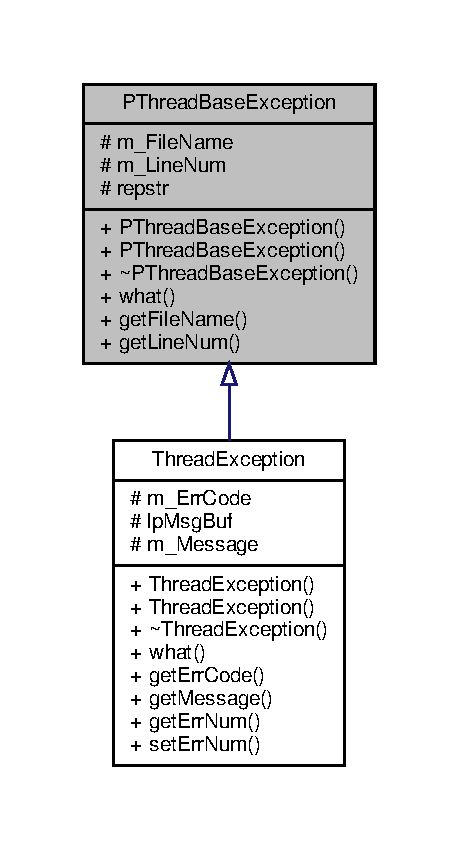
\includegraphics[width=220pt]{classPThreadBaseException__inherit__graph}
\end{center}
\end{figure}
\subsection*{Public Member Functions}
\begin{DoxyCompactItemize}
\item 
\hyperlink{group__EXCEPT__GROUP_ga479c992ccbf4a39cd707a27906925601}{P\+Thread\+Base\+Exception} (const char $\ast$File\+Name, int Line\+Num)
\item 
\hyperlink{group__EXCEPT__GROUP_gaf6dded31d5ab6283d588f99a702241ec}{P\+Thread\+Base\+Exception} (const \hyperlink{classPThreadBaseException}{P\+Thread\+Base\+Exception} \&exp)
\item 
virtual \hyperlink{group__EXCEPT__GROUP_gae4edc60cd7923ef9305a1312cdbc9fc1}{$\sim$\+P\+Thread\+Base\+Exception} ()
\item 
virtual const char $\ast$ \hyperlink{group__EXCEPT__GROUP_ga4389169c01caec3fe93ac45a5d69a9ec}{what} ()
\item 
const char $\ast$ \hyperlink{group__EXCEPT__GROUP_ga4d72952887facf12a96971e964d3427b}{get\+File\+Name} ()
\item 
int \hyperlink{group__EXCEPT__GROUP_ga7a06d992e2dbfa1d283e6c6fb209fd62}{get\+Line\+Num} ()
\end{DoxyCompactItemize}
\subsection*{Protected Attributes}
\begin{DoxyCompactItemize}
\item 
char \hyperlink{group__EXCEPT__GROUP_gace215cb27c8b35eae74d51e9a18f5bfa}{m\+\_\+\+File\+Name} \mbox{[}256\mbox{]}
\begin{DoxyCompactList}\small\item\em Buffer for filename of the exception source. \end{DoxyCompactList}\item 
int \hyperlink{group__EXCEPT__GROUP_ga14fc21c1387d9427ec22d7712c509517}{m\+\_\+\+Line\+Num}
\begin{DoxyCompactList}\small\item\em Line number of the exception source. \end{DoxyCompactList}\item 
std\+::string \hyperlink{group__EXCEPT__GROUP_ga13ce50b63f814e93fc17c484fc28fcd6}{repstr}
\begin{DoxyCompactList}\small\item\em String for the exception report will be build to. \end{DoxyCompactList}\end{DoxyCompactItemize}


\subsection{Detailed Description}
Base class for thread class library exceptions 

The documentation for this class was generated from the following file\+:\begin{DoxyCompactItemize}
\item 
\hyperlink{PThreadBaseException_8h}{P\+Thread\+Base\+Exception.\+h}\end{DoxyCompactItemize}

\hypertarget{classPThreadClass}{}\section{P\+Thread\+Class Class Reference}
\label{classPThreadClass}\index{P\+Thread\+Class@{P\+Thread\+Class}}


{\ttfamily \#include $<$P\+Thread\+Class.\+h$>$}



Inheritance diagram for P\+Thread\+Class\+:\nopagebreak
\begin{figure}[H]
\begin{center}
\leavevmode
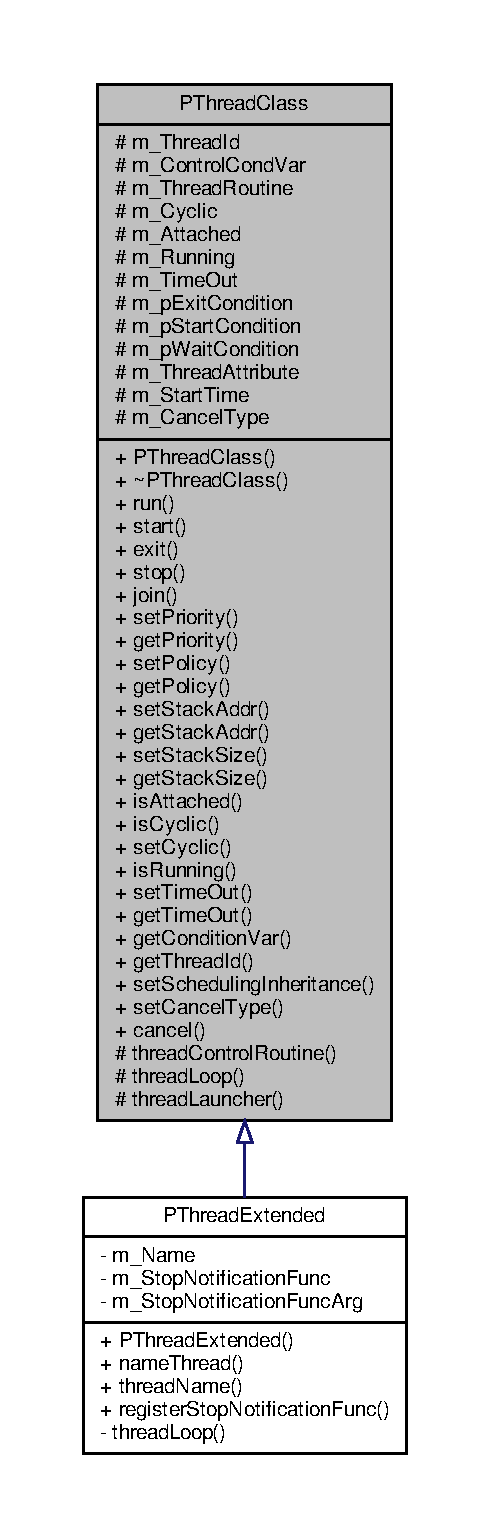
\includegraphics[height=550pt]{classPThreadClass__inherit__graph}
\end{center}
\end{figure}
\subsection*{Public Member Functions}
\begin{DoxyCompactItemize}
\item 
\hyperlink{classPThreadClass_ac0e02c9a05d995e4980837c1491d85e9}{P\+Thread\+Class} (\hyperlink{structRunnable}{Runnable} Routine, unsigned long Time=\hyperlink{PThreadClassLib_8h_a9d2d74d73cb5d069fbfcbcfebf42bd6e}{P\+T\+H\+R\+E\+A\+D\+\_\+\+I\+N\+F\+I\+N\+I\+TE}, bool Cyclic\+Thread=false, bool Attached\+Thread=true) noexcept(false)
\item 
virtual \hyperlink{classPThreadClass_acd1859c3acc32abc90f677578eeb6749}{$\sim$\+P\+Thread\+Class} ()
\begin{DoxyCompactList}\small\item\em Destructor. \end{DoxyCompactList}\item 
virtual bool \hyperlink{classPThreadClass_a9e60b014b8e8ba6892cc322b6ba183d8}{run} () noexcept(false)
\item 
virtual bool \hyperlink{classPThreadClass_a94862a3179469348fd89aefe9dac8244}{start} () noexcept(false)
\item 
virtual bool \hyperlink{classPThreadClass_a699d636eda769173287c18bd1a5f4a77}{exit} () noexcept(false)
\item 
virtual bool \hyperlink{classPThreadClass_a71e308a0324c76e20c504c037a3e7652}{stop} ()
\begin{DoxyCompactList}\small\item\em Stop cyclic execution of thread routine. \end{DoxyCompactList}\item 
virtual bool \hyperlink{classPThreadClass_afe4c0ea5bd3e1c89e01499bbca5e194d}{join} ()
\begin{DoxyCompactList}\small\item\em Join attached thread after. \end{DoxyCompactList}\item 
bool \hyperlink{classPThreadClass_a8d6247e87165abb43186f1a03261f175}{set\+Priority} (int Prio)
\item 
int \hyperlink{classPThreadClass_aca9cc33ac2e0d2f25e1fa993c78e68cc}{get\+Priority} ()
\item 
bool \hyperlink{classPThreadClass_a9fd180b8c007384057618c2c5111e834}{set\+Policy} (int Pol)
\item 
int \hyperlink{classPThreadClass_a8a77ce45b960ad25c2bbdcc4ba8341b6}{get\+Policy} ()
\item 
bool \hyperlink{classPThreadClass_a637580a700f744236440695abe689efa}{set\+Stack\+Addr} (void $\ast$p\+Stack)
\item 
void $\ast$ \hyperlink{classPThreadClass_a0ca8d7ebf843ee190c4cfdfe7909d3f5}{get\+Stack\+Addr} ()
\item 
bool \hyperlink{classPThreadClass_a25c4ea5d463a772ee3b916621e388bed}{set\+Stack\+Size} (size\+\_\+t Stack\+Size)
\item 
size\+\_\+t \hyperlink{classPThreadClass_a2c7527172a945ef9b66f414c142bcefd}{get\+Stack\+Size} ()
\item 
bool \hyperlink{classPThreadClass_af2ad966c36b6995587bde14965722ffc}{is\+Attached} ()
\item 
bool \hyperlink{classPThreadClass_a707a99aa60413db5d6e42230f1f63632}{is\+Cyclic} ()
\item 
void \hyperlink{classPThreadClass_ae217dc6602148a3a5be79089089dc807}{set\+Cyclic} (bool On)
\item 
bool \hyperlink{classPThreadClass_a4f88c65bb031c89b2b0efd31c1c37fc5}{is\+Running} ()
\item 
void \hyperlink{classPThreadClass_a88cda74fba292ade7054204a6833e8ac}{set\+Time\+Out} (unsigned long Time)
\item 
unsigned long \hyperlink{classPThreadClass_accc3e3d98e44796d9f78bc16e22c5403}{get\+Time\+Out} ()
\item 
\hyperlink{classCondVarClass}{Cond\+Var\+Class} \& \hyperlink{classPThreadClass_a9a1dc6820222741276087d0323905b4d}{get\+Condition\+Var} ()
\item 
pthread\+\_\+t \hyperlink{classPThreadClass_a28368c1db23e60e2ab7e12acbd8eef83}{get\+Thread\+Id} ()
\item 
int \hyperlink{classPThreadClass_ad79d5e4fe69d0b77f5c16bf83259c3ad}{set\+Scheduling\+Inheritance} (int Inheritance\+Type)
\item 
void \hyperlink{classPThreadClass_a7d320ee54f3a8f26fc4a3245c36f7df6}{set\+Cancel\+Type} (int Cancel\+Type=P\+T\+H\+R\+E\+A\+D\+\_\+\+C\+A\+N\+C\+E\+L\+\_\+\+D\+E\+F\+E\+R\+R\+ED)
\item 
void \hyperlink{classPThreadClass_a6e4fffd986c68d60ef3c089293007eab}{cancel} ()
\end{DoxyCompactItemize}
\subsection*{Protected Member Functions}
\begin{DoxyCompactItemize}
\item 
virtual void $\ast$ \hyperlink{classPThreadClass_a012fe659b15bb0c0c19125ee0d1fa94e}{thread\+Control\+Routine} ()
\begin{DoxyCompactList}\small\item\em Internal thread routine. \end{DoxyCompactList}\item 
virtual void $\ast$ \hyperlink{classPThreadClass_a77732762f14058291d35bdbbc49018c6}{thread\+Loop} ()
\begin{DoxyCompactList}\small\item\em Internal thread loop. \end{DoxyCompactList}\end{DoxyCompactItemize}
\subsection*{Static Protected Member Functions}
\begin{DoxyCompactItemize}
\item 
static void $\ast$ \hyperlink{classPThreadClass_a0639ba7f95bfe914271a2fe4b61003b1}{thread\+Launcher} (void $\ast$p\+Context)
\begin{DoxyCompactList}\small\item\em Thread launcher. \end{DoxyCompactList}\end{DoxyCompactItemize}
\subsection*{Protected Attributes}
\begin{DoxyCompactItemize}
\item 
pthread\+\_\+t \hyperlink{classPThreadClass_a10ae0a7572009a65e961e14e00368f04}{m\+\_\+\+Thread\+Id}
\begin{DoxyCompactList}\small\item\em P\+O\+S\+IX thread ID. \end{DoxyCompactList}\item 
\hyperlink{classCondVarClass}{Cond\+Var\+Class} \hyperlink{classPThreadClass_a47d4ad65715d6d9bed6987212f05839a}{m\+\_\+\+Control\+Cond\+Var}
\begin{DoxyCompactList}\small\item\em Internal condition variable. \end{DoxyCompactList}\item 
\hyperlink{structRunnable}{Runnable} \hyperlink{classPThreadClass_a80e0b0007257f5c9ef8d74ddacac4113}{m\+\_\+\+Thread\+Routine}
\begin{DoxyCompactList}\small\item\em Thread riotines structure. \end{DoxyCompactList}\item 
volatile bool \hyperlink{classPThreadClass_a6becb8dccddf8546a4091517c1cc5033}{m\+\_\+\+Cyclic}
\begin{DoxyCompactList}\small\item\em Cyclic state. \end{DoxyCompactList}\item 
bool \hyperlink{classPThreadClass_a1905932de950f876dbff1d07e6824954}{m\+\_\+\+Attached}
\begin{DoxyCompactList}\small\item\em Attached state. \end{DoxyCompactList}\item 
bool \hyperlink{classPThreadClass_a390356f43f2203acb2c0abd0f41fe9a1}{m\+\_\+\+Running}
\begin{DoxyCompactList}\small\item\em Running state. \end{DoxyCompactList}\item 
unsigned long \hyperlink{classPThreadClass_a73118712c992ed9921a928cf676bf4d6}{m\+\_\+\+Time\+Out}
\begin{DoxyCompactList}\small\item\em Cyclic period value. \end{DoxyCompactList}\item 
\hyperlink{classSpecificCondition}{Specific\+Condition} $\ast$ \hyperlink{classPThreadClass_a24f676a031214426786294fd15daca30}{m\+\_\+p\+Exit\+Condition}
\begin{DoxyCompactList}\small\item\em Scpecified exit condipion variable. \end{DoxyCompactList}\item 
\hyperlink{classSpecificCondition}{Specific\+Condition} $\ast$ \hyperlink{classPThreadClass_ae7da7ff84d5d96f3dae9d539a0ce8bcb}{m\+\_\+p\+Start\+Condition}
\begin{DoxyCompactList}\small\item\em Scpecified start condipion variable. \end{DoxyCompactList}\item 
\hyperlink{classSpecificCondition}{Specific\+Condition} $\ast$ \hyperlink{classPThreadClass_a1889576909d898228cc4e2eda3acbf8b}{m\+\_\+p\+Wait\+Condition}
\begin{DoxyCompactList}\small\item\em Scpecified wait condipion variable. \end{DoxyCompactList}\item 
pthread\+\_\+attr\+\_\+t \hyperlink{classPThreadClass_a1c637c9e20fb8ccbd8bd9e5431c31883}{m\+\_\+\+Thread\+Attribute}
\begin{DoxyCompactList}\small\item\em P\+O\+S\+IX thread attributes. \end{DoxyCompactList}\item 
struct timeb \hyperlink{classPThreadClass_a21352db28ed04eabcb2d7e353c886319}{m\+\_\+\+Start\+Time}
\begin{DoxyCompactList}\small\item\em Start time of cycle. \end{DoxyCompactList}\item 
int \hyperlink{classPThreadClass_adf415e7e1021b7234ed371744a545daf}{m\+\_\+\+Cancel\+Type}
\end{DoxyCompactItemize}


\subsection{Detailed Description}
P\+O\+S\+IX thread class

Wrapper on P\+O\+S\+IX thread. The thread can be \+: ~\newline
 cyclic / on shot ~\newline
 attached / unattached ~\newline
 bound / unbound to L\+WP (for O\+Ss supporting this) 

\subsection{Constructor \& Destructor Documentation}
\mbox{\Hypertarget{classPThreadClass_ac0e02c9a05d995e4980837c1491d85e9}\label{classPThreadClass_ac0e02c9a05d995e4980837c1491d85e9}} 
\index{P\+Thread\+Class@{P\+Thread\+Class}!P\+Thread\+Class@{P\+Thread\+Class}}
\index{P\+Thread\+Class@{P\+Thread\+Class}!P\+Thread\+Class@{P\+Thread\+Class}}
\subsubsection{\texorpdfstring{P\+Thread\+Class()}{PThreadClass()}}
{\footnotesize\ttfamily P\+Thread\+Class\+::\+P\+Thread\+Class (\begin{DoxyParamCaption}\item[{\hyperlink{structRunnable}{Runnable}}]{Routine,  }\item[{unsigned long}]{Time = {\ttfamily \hyperlink{PThreadClassLib_8h_a9d2d74d73cb5d069fbfcbcfebf42bd6e}{P\+T\+H\+R\+E\+A\+D\+\_\+\+I\+N\+F\+I\+N\+I\+TE}},  }\item[{bool}]{Cyclic\+Thread = {\ttfamily false},  }\item[{bool}]{Attached\+Thread = {\ttfamily true} }\end{DoxyParamCaption})\hspace{0.3cm}{\ttfamily [noexcept]}}

Constructor 
\begin{DoxyParams}{Parameters}
{\em Routine} & \+: routines structure reference. \\
\hline
{\em Time} & \+: cyclic period value in milliseconds. \\
\hline
{\em Cyclic\+Thread} & \+: cyclic (true) or one-\/shot (false) thread. \\
\hline
{\em Attached\+Thread} & \+: attached (true) or unattached (false) thread. \\
\hline
{\em Bound\+Thread} & \+: binding to L\+WP flag. Applicable only on supporting binding O\+Ss. \\
\hline
\end{DoxyParams}

\begin{DoxyExceptions}{Exceptions}
{\em \hyperlink{classThreadException}{Thread\+Exception}} & \\
\hline
\end{DoxyExceptions}
\mbox{\Hypertarget{classPThreadClass_acd1859c3acc32abc90f677578eeb6749}\label{classPThreadClass_acd1859c3acc32abc90f677578eeb6749}} 
\index{P\+Thread\+Class@{P\+Thread\+Class}!````~P\+Thread\+Class@{$\sim$\+P\+Thread\+Class}}
\index{````~P\+Thread\+Class@{$\sim$\+P\+Thread\+Class}!P\+Thread\+Class@{P\+Thread\+Class}}
\subsubsection{\texorpdfstring{$\sim$\+P\+Thread\+Class()}{~PThreadClass()}}
{\footnotesize\ttfamily P\+Thread\+Class\+::$\sim$\+P\+Thread\+Class (\begin{DoxyParamCaption}{ }\end{DoxyParamCaption})\hspace{0.3cm}{\ttfamily [virtual]}}



Destructor. 



\subsection{Member Function Documentation}
\mbox{\Hypertarget{classPThreadClass_a6e4fffd986c68d60ef3c089293007eab}\label{classPThreadClass_a6e4fffd986c68d60ef3c089293007eab}} 
\index{P\+Thread\+Class@{P\+Thread\+Class}!cancel@{cancel}}
\index{cancel@{cancel}!P\+Thread\+Class@{P\+Thread\+Class}}
\subsubsection{\texorpdfstring{cancel()}{cancel()}}
{\footnotesize\ttfamily void P\+Thread\+Class\+::cancel (\begin{DoxyParamCaption}{ }\end{DoxyParamCaption})\hspace{0.3cm}{\ttfamily [inline]}}

\mbox{\Hypertarget{classPThreadClass_a699d636eda769173287c18bd1a5f4a77}\label{classPThreadClass_a699d636eda769173287c18bd1a5f4a77}} 
\index{P\+Thread\+Class@{P\+Thread\+Class}!exit@{exit}}
\index{exit@{exit}!P\+Thread\+Class@{P\+Thread\+Class}}
\subsubsection{\texorpdfstring{exit()}{exit()}}
{\footnotesize\ttfamily bool P\+Thread\+Class\+::exit (\begin{DoxyParamCaption}{ }\end{DoxyParamCaption})\hspace{0.3cm}{\ttfamily [virtual]}, {\ttfamily [noexcept]}}

Destroy thread. 
\begin{DoxyExceptions}{Exceptions}
{\em \hyperlink{classThreadException}{Thread\+Exception}} & \\
\hline
\end{DoxyExceptions}
\mbox{\Hypertarget{classPThreadClass_a9a1dc6820222741276087d0323905b4d}\label{classPThreadClass_a9a1dc6820222741276087d0323905b4d}} 
\index{P\+Thread\+Class@{P\+Thread\+Class}!get\+Condition\+Var@{get\+Condition\+Var}}
\index{get\+Condition\+Var@{get\+Condition\+Var}!P\+Thread\+Class@{P\+Thread\+Class}}
\subsubsection{\texorpdfstring{get\+Condition\+Var()}{getConditionVar()}}
{\footnotesize\ttfamily \hyperlink{classCondVarClass}{Cond\+Var\+Class}\& P\+Thread\+Class\+::get\+Condition\+Var (\begin{DoxyParamCaption}{ }\end{DoxyParamCaption})\hspace{0.3cm}{\ttfamily [inline]}}

Get reference on internal condition variable. \begin{DoxyReturn}{Returns}
reference on internal condition variable. 
\end{DoxyReturn}
\mbox{\Hypertarget{classPThreadClass_a8a77ce45b960ad25c2bbdcc4ba8341b6}\label{classPThreadClass_a8a77ce45b960ad25c2bbdcc4ba8341b6}} 
\index{P\+Thread\+Class@{P\+Thread\+Class}!get\+Policy@{get\+Policy}}
\index{get\+Policy@{get\+Policy}!P\+Thread\+Class@{P\+Thread\+Class}}
\subsubsection{\texorpdfstring{get\+Policy()}{getPolicy()}}
{\footnotesize\ttfamily int P\+Thread\+Class\+::get\+Policy (\begin{DoxyParamCaption}{ }\end{DoxyParamCaption})}

Get P\+O\+S\+IX priority level.

should be called after \hyperlink{classPThreadClass_a9e60b014b8e8ba6892cc322b6ba183d8}{run()}. \begin{DoxyReturn}{Returns}
policy or -\/1 on failure. 
\end{DoxyReturn}
\mbox{\Hypertarget{classPThreadClass_aca9cc33ac2e0d2f25e1fa993c78e68cc}\label{classPThreadClass_aca9cc33ac2e0d2f25e1fa993c78e68cc}} 
\index{P\+Thread\+Class@{P\+Thread\+Class}!get\+Priority@{get\+Priority}}
\index{get\+Priority@{get\+Priority}!P\+Thread\+Class@{P\+Thread\+Class}}
\subsubsection{\texorpdfstring{get\+Priority()}{getPriority()}}
{\footnotesize\ttfamily int P\+Thread\+Class\+::get\+Priority (\begin{DoxyParamCaption}{ }\end{DoxyParamCaption})}

Get P\+O\+S\+IX priority level.

should be called after \hyperlink{classPThreadClass_a9e60b014b8e8ba6892cc322b6ba183d8}{run()}. \begin{DoxyReturn}{Returns}
priority level or -\/1 on failure. 
\end{DoxyReturn}
\mbox{\Hypertarget{classPThreadClass_a0ca8d7ebf843ee190c4cfdfe7909d3f5}\label{classPThreadClass_a0ca8d7ebf843ee190c4cfdfe7909d3f5}} 
\index{P\+Thread\+Class@{P\+Thread\+Class}!get\+Stack\+Addr@{get\+Stack\+Addr}}
\index{get\+Stack\+Addr@{get\+Stack\+Addr}!P\+Thread\+Class@{P\+Thread\+Class}}
\subsubsection{\texorpdfstring{get\+Stack\+Addr()}{getStackAddr()}}
{\footnotesize\ttfamily void $\ast$ P\+Thread\+Class\+::get\+Stack\+Addr (\begin{DoxyParamCaption}{ }\end{DoxyParamCaption})}

Get thread stack address.

should be called after \hyperlink{classPThreadClass_a9e60b014b8e8ba6892cc322b6ba183d8}{run()}. \begin{DoxyReturn}{Returns}
stack address or -\/1 on failure. 
\end{DoxyReturn}
\mbox{\Hypertarget{classPThreadClass_a2c7527172a945ef9b66f414c142bcefd}\label{classPThreadClass_a2c7527172a945ef9b66f414c142bcefd}} 
\index{P\+Thread\+Class@{P\+Thread\+Class}!get\+Stack\+Size@{get\+Stack\+Size}}
\index{get\+Stack\+Size@{get\+Stack\+Size}!P\+Thread\+Class@{P\+Thread\+Class}}
\subsubsection{\texorpdfstring{get\+Stack\+Size()}{getStackSize()}}
{\footnotesize\ttfamily size\+\_\+t P\+Thread\+Class\+::get\+Stack\+Size (\begin{DoxyParamCaption}{ }\end{DoxyParamCaption})}

Get thread stack size. \begin{DoxyReturn}{Returns}
stack size or -\/1 on failure. 
\end{DoxyReturn}
\mbox{\Hypertarget{classPThreadClass_a28368c1db23e60e2ab7e12acbd8eef83}\label{classPThreadClass_a28368c1db23e60e2ab7e12acbd8eef83}} 
\index{P\+Thread\+Class@{P\+Thread\+Class}!get\+Thread\+Id@{get\+Thread\+Id}}
\index{get\+Thread\+Id@{get\+Thread\+Id}!P\+Thread\+Class@{P\+Thread\+Class}}
\subsubsection{\texorpdfstring{get\+Thread\+Id()}{getThreadId()}}
{\footnotesize\ttfamily pthread\+\_\+t P\+Thread\+Class\+::get\+Thread\+Id (\begin{DoxyParamCaption}{ }\end{DoxyParamCaption})\hspace{0.3cm}{\ttfamily [inline]}}

Get P\+O\+S\+IX thread ID.

should be called after \hyperlink{classPThreadClass_a9e60b014b8e8ba6892cc322b6ba183d8}{run()}. \begin{DoxyReturn}{Returns}
P\+O\+S\+IX thread ID. 
\end{DoxyReturn}
\mbox{\Hypertarget{classPThreadClass_accc3e3d98e44796d9f78bc16e22c5403}\label{classPThreadClass_accc3e3d98e44796d9f78bc16e22c5403}} 
\index{P\+Thread\+Class@{P\+Thread\+Class}!get\+Time\+Out@{get\+Time\+Out}}
\index{get\+Time\+Out@{get\+Time\+Out}!P\+Thread\+Class@{P\+Thread\+Class}}
\subsubsection{\texorpdfstring{get\+Time\+Out()}{getTimeOut()}}
{\footnotesize\ttfamily unsigned long P\+Thread\+Class\+::get\+Time\+Out (\begin{DoxyParamCaption}{ }\end{DoxyParamCaption})\hspace{0.3cm}{\ttfamily [inline]}}

Get cyclic period value. \begin{DoxyReturn}{Returns}
cyclic period in milliseconds. 
\end{DoxyReturn}
\mbox{\Hypertarget{classPThreadClass_af2ad966c36b6995587bde14965722ffc}\label{classPThreadClass_af2ad966c36b6995587bde14965722ffc}} 
\index{P\+Thread\+Class@{P\+Thread\+Class}!is\+Attached@{is\+Attached}}
\index{is\+Attached@{is\+Attached}!P\+Thread\+Class@{P\+Thread\+Class}}
\subsubsection{\texorpdfstring{is\+Attached()}{isAttached()}}
{\footnotesize\ttfamily bool P\+Thread\+Class\+::is\+Attached (\begin{DoxyParamCaption}{ }\end{DoxyParamCaption})\hspace{0.3cm}{\ttfamily [inline]}}

Is thread attached? \begin{DoxyReturn}{Returns}
attached state. 
\end{DoxyReturn}
\mbox{\Hypertarget{classPThreadClass_a707a99aa60413db5d6e42230f1f63632}\label{classPThreadClass_a707a99aa60413db5d6e42230f1f63632}} 
\index{P\+Thread\+Class@{P\+Thread\+Class}!is\+Cyclic@{is\+Cyclic}}
\index{is\+Cyclic@{is\+Cyclic}!P\+Thread\+Class@{P\+Thread\+Class}}
\subsubsection{\texorpdfstring{is\+Cyclic()}{isCyclic()}}
{\footnotesize\ttfamily bool P\+Thread\+Class\+::is\+Cyclic (\begin{DoxyParamCaption}{ }\end{DoxyParamCaption})\hspace{0.3cm}{\ttfamily [inline]}}

Is thread cyclic? \begin{DoxyReturn}{Returns}
cyclic state. 
\end{DoxyReturn}
\mbox{\Hypertarget{classPThreadClass_a4f88c65bb031c89b2b0efd31c1c37fc5}\label{classPThreadClass_a4f88c65bb031c89b2b0efd31c1c37fc5}} 
\index{P\+Thread\+Class@{P\+Thread\+Class}!is\+Running@{is\+Running}}
\index{is\+Running@{is\+Running}!P\+Thread\+Class@{P\+Thread\+Class}}
\subsubsection{\texorpdfstring{is\+Running()}{isRunning()}}
{\footnotesize\ttfamily bool P\+Thread\+Class\+::is\+Running (\begin{DoxyParamCaption}{ }\end{DoxyParamCaption})\hspace{0.3cm}{\ttfamily [inline]}}

Is thread ready for execution? \begin{DoxyReturn}{Returns}
running state. 
\end{DoxyReturn}
\mbox{\Hypertarget{classPThreadClass_afe4c0ea5bd3e1c89e01499bbca5e194d}\label{classPThreadClass_afe4c0ea5bd3e1c89e01499bbca5e194d}} 
\index{P\+Thread\+Class@{P\+Thread\+Class}!join@{join}}
\index{join@{join}!P\+Thread\+Class@{P\+Thread\+Class}}
\subsubsection{\texorpdfstring{join()}{join()}}
{\footnotesize\ttfamily bool P\+Thread\+Class\+::join (\begin{DoxyParamCaption}{ }\end{DoxyParamCaption})\hspace{0.3cm}{\ttfamily [virtual]}}



Join attached thread after. 

\mbox{\Hypertarget{classPThreadClass_a9e60b014b8e8ba6892cc322b6ba183d8}\label{classPThreadClass_a9e60b014b8e8ba6892cc322b6ba183d8}} 
\index{P\+Thread\+Class@{P\+Thread\+Class}!run@{run}}
\index{run@{run}!P\+Thread\+Class@{P\+Thread\+Class}}
\subsubsection{\texorpdfstring{run()}{run()}}
{\footnotesize\ttfamily bool P\+Thread\+Class\+::run (\begin{DoxyParamCaption}{ }\end{DoxyParamCaption})\hspace{0.3cm}{\ttfamily [virtual]}, {\ttfamily [noexcept]}}

Initialize and run thread, make it ready to execute thread routine. 
\begin{DoxyExceptions}{Exceptions}
{\em \hyperlink{classThreadException}{Thread\+Exception}} & \\
\hline
\end{DoxyExceptions}
\mbox{\Hypertarget{classPThreadClass_a7d320ee54f3a8f26fc4a3245c36f7df6}\label{classPThreadClass_a7d320ee54f3a8f26fc4a3245c36f7df6}} 
\index{P\+Thread\+Class@{P\+Thread\+Class}!set\+Cancel\+Type@{set\+Cancel\+Type}}
\index{set\+Cancel\+Type@{set\+Cancel\+Type}!P\+Thread\+Class@{P\+Thread\+Class}}
\subsubsection{\texorpdfstring{set\+Cancel\+Type()}{setCancelType()}}
{\footnotesize\ttfamily void P\+Thread\+Class\+::set\+Cancel\+Type (\begin{DoxyParamCaption}\item[{int}]{Cancel\+Type = {\ttfamily PTHREAD\+\_\+CANCEL\+\_\+DEFERRED} }\end{DoxyParamCaption})\hspace{0.3cm}{\ttfamily [inline]}}

\mbox{\Hypertarget{classPThreadClass_ae217dc6602148a3a5be79089089dc807}\label{classPThreadClass_ae217dc6602148a3a5be79089089dc807}} 
\index{P\+Thread\+Class@{P\+Thread\+Class}!set\+Cyclic@{set\+Cyclic}}
\index{set\+Cyclic@{set\+Cyclic}!P\+Thread\+Class@{P\+Thread\+Class}}
\subsubsection{\texorpdfstring{set\+Cyclic()}{setCyclic()}}
{\footnotesize\ttfamily void P\+Thread\+Class\+::set\+Cyclic (\begin{DoxyParamCaption}\item[{bool}]{On }\end{DoxyParamCaption})}

Set thread cyclic state. 
\begin{DoxyParams}{Parameters}
{\em On} & \+: true or false. \\
\hline
\end{DoxyParams}
\mbox{\Hypertarget{classPThreadClass_a9fd180b8c007384057618c2c5111e834}\label{classPThreadClass_a9fd180b8c007384057618c2c5111e834}} 
\index{P\+Thread\+Class@{P\+Thread\+Class}!set\+Policy@{set\+Policy}}
\index{set\+Policy@{set\+Policy}!P\+Thread\+Class@{P\+Thread\+Class}}
\subsubsection{\texorpdfstring{set\+Policy()}{setPolicy()}}
{\footnotesize\ttfamily bool P\+Thread\+Class\+::set\+Policy (\begin{DoxyParamCaption}\item[{int}]{Pol }\end{DoxyParamCaption})}

Set thread scheduling policy.

should be called before \hyperlink{classPThreadClass_a9e60b014b8e8ba6892cc322b6ba183d8}{run()}. \begin{DoxyReturn}{Returns}
success or fail of the operation. 
\end{DoxyReturn}

\begin{DoxyParams}{Parameters}
{\em Pol} & \+: P\+O\+S\+IX scheduling policy. \\
\hline
\end{DoxyParams}
\mbox{\Hypertarget{classPThreadClass_a8d6247e87165abb43186f1a03261f175}\label{classPThreadClass_a8d6247e87165abb43186f1a03261f175}} 
\index{P\+Thread\+Class@{P\+Thread\+Class}!set\+Priority@{set\+Priority}}
\index{set\+Priority@{set\+Priority}!P\+Thread\+Class@{P\+Thread\+Class}}
\subsubsection{\texorpdfstring{set\+Priority()}{setPriority()}}
{\footnotesize\ttfamily bool P\+Thread\+Class\+::set\+Priority (\begin{DoxyParamCaption}\item[{int}]{Prio }\end{DoxyParamCaption})}

Set thread priority. \begin{DoxyReturn}{Returns}
success or fail of the operation. 
\end{DoxyReturn}

\begin{DoxyParams}{Parameters}
{\em Prio} & \+: P\+O\+S\+IX priority level. \\
\hline
\end{DoxyParams}
\mbox{\Hypertarget{classPThreadClass_ad79d5e4fe69d0b77f5c16bf83259c3ad}\label{classPThreadClass_ad79d5e4fe69d0b77f5c16bf83259c3ad}} 
\index{P\+Thread\+Class@{P\+Thread\+Class}!set\+Scheduling\+Inheritance@{set\+Scheduling\+Inheritance}}
\index{set\+Scheduling\+Inheritance@{set\+Scheduling\+Inheritance}!P\+Thread\+Class@{P\+Thread\+Class}}
\subsubsection{\texorpdfstring{set\+Scheduling\+Inheritance()}{setSchedulingInheritance()}}
{\footnotesize\ttfamily int P\+Thread\+Class\+::set\+Scheduling\+Inheritance (\begin{DoxyParamCaption}\item[{int}]{Inheritance\+Type }\end{DoxyParamCaption})\hspace{0.3cm}{\ttfamily [inline]}}

Scheduling policy inheritance setting

should be called after \hyperlink{classPThreadClass_a9e60b014b8e8ba6892cc322b6ba183d8}{run()}. 
\begin{DoxyParams}{Parameters}
{\em Inheritance\+Type} & \+: scheduling policy inheritance type P\+T\+H\+R\+E\+A\+D\+\_\+\+I\+N\+H\+E\+R\+I\+T\+\_\+\+S\+C\+H\+ED or P\+T\+H\+R\+E\+A\+D\+\_\+\+E\+X\+P\+L\+I\+C\+I\+T\+\_\+\+S\+C\+H\+ED. \\
\hline
\end{DoxyParams}
\mbox{\Hypertarget{classPThreadClass_a637580a700f744236440695abe689efa}\label{classPThreadClass_a637580a700f744236440695abe689efa}} 
\index{P\+Thread\+Class@{P\+Thread\+Class}!set\+Stack\+Addr@{set\+Stack\+Addr}}
\index{set\+Stack\+Addr@{set\+Stack\+Addr}!P\+Thread\+Class@{P\+Thread\+Class}}
\subsubsection{\texorpdfstring{set\+Stack\+Addr()}{setStackAddr()}}
{\footnotesize\ttfamily bool P\+Thread\+Class\+::set\+Stack\+Addr (\begin{DoxyParamCaption}\item[{void $\ast$}]{p\+Stack }\end{DoxyParamCaption})}

Set thread stack address.

should be called before \hyperlink{classPThreadClass_a9e60b014b8e8ba6892cc322b6ba183d8}{run()}. \begin{DoxyReturn}{Returns}
success or fail of the operation. 
\end{DoxyReturn}

\begin{DoxyParams}{Parameters}
{\em p\+Stack} & \+: stack address. \\
\hline
\end{DoxyParams}
\mbox{\Hypertarget{classPThreadClass_a25c4ea5d463a772ee3b916621e388bed}\label{classPThreadClass_a25c4ea5d463a772ee3b916621e388bed}} 
\index{P\+Thread\+Class@{P\+Thread\+Class}!set\+Stack\+Size@{set\+Stack\+Size}}
\index{set\+Stack\+Size@{set\+Stack\+Size}!P\+Thread\+Class@{P\+Thread\+Class}}
\subsubsection{\texorpdfstring{set\+Stack\+Size()}{setStackSize()}}
{\footnotesize\ttfamily bool P\+Thread\+Class\+::set\+Stack\+Size (\begin{DoxyParamCaption}\item[{size\+\_\+t}]{Stack\+Size }\end{DoxyParamCaption})}

Set thread stack address.

should be called before \hyperlink{classPThreadClass_a9e60b014b8e8ba6892cc322b6ba183d8}{run()}. \begin{DoxyReturn}{Returns}
success or fail of the operation. 
\end{DoxyReturn}

\begin{DoxyParams}{Parameters}
{\em p\+Stack} & \+: stack address. \\
\hline
\end{DoxyParams}
\mbox{\Hypertarget{classPThreadClass_a88cda74fba292ade7054204a6833e8ac}\label{classPThreadClass_a88cda74fba292ade7054204a6833e8ac}} 
\index{P\+Thread\+Class@{P\+Thread\+Class}!set\+Time\+Out@{set\+Time\+Out}}
\index{set\+Time\+Out@{set\+Time\+Out}!P\+Thread\+Class@{P\+Thread\+Class}}
\subsubsection{\texorpdfstring{set\+Time\+Out()}{setTimeOut()}}
{\footnotesize\ttfamily void P\+Thread\+Class\+::set\+Time\+Out (\begin{DoxyParamCaption}\item[{unsigned long}]{Time }\end{DoxyParamCaption})\hspace{0.3cm}{\ttfamily [inline]}}

Set cyclic period. 
\begin{DoxyParams}{Parameters}
{\em Time} & \+: cyclic period in milliseconds. \\
\hline
\end{DoxyParams}
\mbox{\Hypertarget{classPThreadClass_a94862a3179469348fd89aefe9dac8244}\label{classPThreadClass_a94862a3179469348fd89aefe9dac8244}} 
\index{P\+Thread\+Class@{P\+Thread\+Class}!start@{start}}
\index{start@{start}!P\+Thread\+Class@{P\+Thread\+Class}}
\subsubsection{\texorpdfstring{start()}{start()}}
{\footnotesize\ttfamily bool P\+Thread\+Class\+::start (\begin{DoxyParamCaption}{ }\end{DoxyParamCaption})\hspace{0.3cm}{\ttfamily [virtual]}, {\ttfamily [noexcept]}}

Start execution of thread routine. 
\begin{DoxyExceptions}{Exceptions}
{\em \hyperlink{classThreadException}{Thread\+Exception}} & \\
\hline
\end{DoxyExceptions}
\mbox{\Hypertarget{classPThreadClass_a71e308a0324c76e20c504c037a3e7652}\label{classPThreadClass_a71e308a0324c76e20c504c037a3e7652}} 
\index{P\+Thread\+Class@{P\+Thread\+Class}!stop@{stop}}
\index{stop@{stop}!P\+Thread\+Class@{P\+Thread\+Class}}
\subsubsection{\texorpdfstring{stop()}{stop()}}
{\footnotesize\ttfamily bool P\+Thread\+Class\+::stop (\begin{DoxyParamCaption}{ }\end{DoxyParamCaption})\hspace{0.3cm}{\ttfamily [virtual]}}



Stop cyclic execution of thread routine. 

\mbox{\Hypertarget{classPThreadClass_a012fe659b15bb0c0c19125ee0d1fa94e}\label{classPThreadClass_a012fe659b15bb0c0c19125ee0d1fa94e}} 
\index{P\+Thread\+Class@{P\+Thread\+Class}!thread\+Control\+Routine@{thread\+Control\+Routine}}
\index{thread\+Control\+Routine@{thread\+Control\+Routine}!P\+Thread\+Class@{P\+Thread\+Class}}
\subsubsection{\texorpdfstring{thread\+Control\+Routine()}{threadControlRoutine()}}
{\footnotesize\ttfamily void $\ast$ P\+Thread\+Class\+::thread\+Control\+Routine (\begin{DoxyParamCaption}{ }\end{DoxyParamCaption})\hspace{0.3cm}{\ttfamily [protected]}, {\ttfamily [virtual]}}



Internal thread routine. 

\mbox{\Hypertarget{classPThreadClass_a0639ba7f95bfe914271a2fe4b61003b1}\label{classPThreadClass_a0639ba7f95bfe914271a2fe4b61003b1}} 
\index{P\+Thread\+Class@{P\+Thread\+Class}!thread\+Launcher@{thread\+Launcher}}
\index{thread\+Launcher@{thread\+Launcher}!P\+Thread\+Class@{P\+Thread\+Class}}
\subsubsection{\texorpdfstring{thread\+Launcher()}{threadLauncher()}}
{\footnotesize\ttfamily static void$\ast$ P\+Thread\+Class\+::thread\+Launcher (\begin{DoxyParamCaption}\item[{void $\ast$}]{p\+Context }\end{DoxyParamCaption})\hspace{0.3cm}{\ttfamily [inline]}, {\ttfamily [static]}, {\ttfamily [protected]}}



Thread launcher. 

\mbox{\Hypertarget{classPThreadClass_a77732762f14058291d35bdbbc49018c6}\label{classPThreadClass_a77732762f14058291d35bdbbc49018c6}} 
\index{P\+Thread\+Class@{P\+Thread\+Class}!thread\+Loop@{thread\+Loop}}
\index{thread\+Loop@{thread\+Loop}!P\+Thread\+Class@{P\+Thread\+Class}}
\subsubsection{\texorpdfstring{thread\+Loop()}{threadLoop()}}
{\footnotesize\ttfamily void $\ast$ P\+Thread\+Class\+::thread\+Loop (\begin{DoxyParamCaption}{ }\end{DoxyParamCaption})\hspace{0.3cm}{\ttfamily [protected]}, {\ttfamily [virtual]}}



Internal thread loop. 



Reimplemented in \hyperlink{classPThreadExtended_a43d31ca653ffe314e400a48a77f8e0a9}{P\+Thread\+Extended}.



\subsection{Member Data Documentation}
\mbox{\Hypertarget{classPThreadClass_a1905932de950f876dbff1d07e6824954}\label{classPThreadClass_a1905932de950f876dbff1d07e6824954}} 
\index{P\+Thread\+Class@{P\+Thread\+Class}!m\+\_\+\+Attached@{m\+\_\+\+Attached}}
\index{m\+\_\+\+Attached@{m\+\_\+\+Attached}!P\+Thread\+Class@{P\+Thread\+Class}}
\subsubsection{\texorpdfstring{m\+\_\+\+Attached}{m\_Attached}}
{\footnotesize\ttfamily bool P\+Thread\+Class\+::m\+\_\+\+Attached\hspace{0.3cm}{\ttfamily [protected]}}



Attached state. 

\mbox{\Hypertarget{classPThreadClass_adf415e7e1021b7234ed371744a545daf}\label{classPThreadClass_adf415e7e1021b7234ed371744a545daf}} 
\index{P\+Thread\+Class@{P\+Thread\+Class}!m\+\_\+\+Cancel\+Type@{m\+\_\+\+Cancel\+Type}}
\index{m\+\_\+\+Cancel\+Type@{m\+\_\+\+Cancel\+Type}!P\+Thread\+Class@{P\+Thread\+Class}}
\subsubsection{\texorpdfstring{m\+\_\+\+Cancel\+Type}{m\_CancelType}}
{\footnotesize\ttfamily int P\+Thread\+Class\+::m\+\_\+\+Cancel\+Type\hspace{0.3cm}{\ttfamily [protected]}}

\mbox{\Hypertarget{classPThreadClass_a47d4ad65715d6d9bed6987212f05839a}\label{classPThreadClass_a47d4ad65715d6d9bed6987212f05839a}} 
\index{P\+Thread\+Class@{P\+Thread\+Class}!m\+\_\+\+Control\+Cond\+Var@{m\+\_\+\+Control\+Cond\+Var}}
\index{m\+\_\+\+Control\+Cond\+Var@{m\+\_\+\+Control\+Cond\+Var}!P\+Thread\+Class@{P\+Thread\+Class}}
\subsubsection{\texorpdfstring{m\+\_\+\+Control\+Cond\+Var}{m\_ControlCondVar}}
{\footnotesize\ttfamily \hyperlink{classCondVarClass}{Cond\+Var\+Class} P\+Thread\+Class\+::m\+\_\+\+Control\+Cond\+Var\hspace{0.3cm}{\ttfamily [protected]}}



Internal condition variable. 

\mbox{\Hypertarget{classPThreadClass_a6becb8dccddf8546a4091517c1cc5033}\label{classPThreadClass_a6becb8dccddf8546a4091517c1cc5033}} 
\index{P\+Thread\+Class@{P\+Thread\+Class}!m\+\_\+\+Cyclic@{m\+\_\+\+Cyclic}}
\index{m\+\_\+\+Cyclic@{m\+\_\+\+Cyclic}!P\+Thread\+Class@{P\+Thread\+Class}}
\subsubsection{\texorpdfstring{m\+\_\+\+Cyclic}{m\_Cyclic}}
{\footnotesize\ttfamily volatile bool P\+Thread\+Class\+::m\+\_\+\+Cyclic\hspace{0.3cm}{\ttfamily [protected]}}



Cyclic state. 

\mbox{\Hypertarget{classPThreadClass_a24f676a031214426786294fd15daca30}\label{classPThreadClass_a24f676a031214426786294fd15daca30}} 
\index{P\+Thread\+Class@{P\+Thread\+Class}!m\+\_\+p\+Exit\+Condition@{m\+\_\+p\+Exit\+Condition}}
\index{m\+\_\+p\+Exit\+Condition@{m\+\_\+p\+Exit\+Condition}!P\+Thread\+Class@{P\+Thread\+Class}}
\subsubsection{\texorpdfstring{m\+\_\+p\+Exit\+Condition}{m\_pExitCondition}}
{\footnotesize\ttfamily \hyperlink{classSpecificCondition}{Specific\+Condition}$\ast$ P\+Thread\+Class\+::m\+\_\+p\+Exit\+Condition\hspace{0.3cm}{\ttfamily [protected]}}



Scpecified exit condipion variable. 

\mbox{\Hypertarget{classPThreadClass_ae7da7ff84d5d96f3dae9d539a0ce8bcb}\label{classPThreadClass_ae7da7ff84d5d96f3dae9d539a0ce8bcb}} 
\index{P\+Thread\+Class@{P\+Thread\+Class}!m\+\_\+p\+Start\+Condition@{m\+\_\+p\+Start\+Condition}}
\index{m\+\_\+p\+Start\+Condition@{m\+\_\+p\+Start\+Condition}!P\+Thread\+Class@{P\+Thread\+Class}}
\subsubsection{\texorpdfstring{m\+\_\+p\+Start\+Condition}{m\_pStartCondition}}
{\footnotesize\ttfamily \hyperlink{classSpecificCondition}{Specific\+Condition}$\ast$ P\+Thread\+Class\+::m\+\_\+p\+Start\+Condition\hspace{0.3cm}{\ttfamily [protected]}}



Scpecified start condipion variable. 

\mbox{\Hypertarget{classPThreadClass_a1889576909d898228cc4e2eda3acbf8b}\label{classPThreadClass_a1889576909d898228cc4e2eda3acbf8b}} 
\index{P\+Thread\+Class@{P\+Thread\+Class}!m\+\_\+p\+Wait\+Condition@{m\+\_\+p\+Wait\+Condition}}
\index{m\+\_\+p\+Wait\+Condition@{m\+\_\+p\+Wait\+Condition}!P\+Thread\+Class@{P\+Thread\+Class}}
\subsubsection{\texorpdfstring{m\+\_\+p\+Wait\+Condition}{m\_pWaitCondition}}
{\footnotesize\ttfamily \hyperlink{classSpecificCondition}{Specific\+Condition}$\ast$ P\+Thread\+Class\+::m\+\_\+p\+Wait\+Condition\hspace{0.3cm}{\ttfamily [protected]}}



Scpecified wait condipion variable. 

\mbox{\Hypertarget{classPThreadClass_a390356f43f2203acb2c0abd0f41fe9a1}\label{classPThreadClass_a390356f43f2203acb2c0abd0f41fe9a1}} 
\index{P\+Thread\+Class@{P\+Thread\+Class}!m\+\_\+\+Running@{m\+\_\+\+Running}}
\index{m\+\_\+\+Running@{m\+\_\+\+Running}!P\+Thread\+Class@{P\+Thread\+Class}}
\subsubsection{\texorpdfstring{m\+\_\+\+Running}{m\_Running}}
{\footnotesize\ttfamily bool P\+Thread\+Class\+::m\+\_\+\+Running\hspace{0.3cm}{\ttfamily [protected]}}



Running state. 

\mbox{\Hypertarget{classPThreadClass_a21352db28ed04eabcb2d7e353c886319}\label{classPThreadClass_a21352db28ed04eabcb2d7e353c886319}} 
\index{P\+Thread\+Class@{P\+Thread\+Class}!m\+\_\+\+Start\+Time@{m\+\_\+\+Start\+Time}}
\index{m\+\_\+\+Start\+Time@{m\+\_\+\+Start\+Time}!P\+Thread\+Class@{P\+Thread\+Class}}
\subsubsection{\texorpdfstring{m\+\_\+\+Start\+Time}{m\_StartTime}}
{\footnotesize\ttfamily struct timeb P\+Thread\+Class\+::m\+\_\+\+Start\+Time\hspace{0.3cm}{\ttfamily [protected]}}



Start time of cycle. 

\mbox{\Hypertarget{classPThreadClass_a1c637c9e20fb8ccbd8bd9e5431c31883}\label{classPThreadClass_a1c637c9e20fb8ccbd8bd9e5431c31883}} 
\index{P\+Thread\+Class@{P\+Thread\+Class}!m\+\_\+\+Thread\+Attribute@{m\+\_\+\+Thread\+Attribute}}
\index{m\+\_\+\+Thread\+Attribute@{m\+\_\+\+Thread\+Attribute}!P\+Thread\+Class@{P\+Thread\+Class}}
\subsubsection{\texorpdfstring{m\+\_\+\+Thread\+Attribute}{m\_ThreadAttribute}}
{\footnotesize\ttfamily pthread\+\_\+attr\+\_\+t P\+Thread\+Class\+::m\+\_\+\+Thread\+Attribute\hspace{0.3cm}{\ttfamily [protected]}}



P\+O\+S\+IX thread attributes. 

\mbox{\Hypertarget{classPThreadClass_a10ae0a7572009a65e961e14e00368f04}\label{classPThreadClass_a10ae0a7572009a65e961e14e00368f04}} 
\index{P\+Thread\+Class@{P\+Thread\+Class}!m\+\_\+\+Thread\+Id@{m\+\_\+\+Thread\+Id}}
\index{m\+\_\+\+Thread\+Id@{m\+\_\+\+Thread\+Id}!P\+Thread\+Class@{P\+Thread\+Class}}
\subsubsection{\texorpdfstring{m\+\_\+\+Thread\+Id}{m\_ThreadId}}
{\footnotesize\ttfamily pthread\+\_\+t P\+Thread\+Class\+::m\+\_\+\+Thread\+Id\hspace{0.3cm}{\ttfamily [protected]}}



P\+O\+S\+IX thread ID. 

\mbox{\Hypertarget{classPThreadClass_a80e0b0007257f5c9ef8d74ddacac4113}\label{classPThreadClass_a80e0b0007257f5c9ef8d74ddacac4113}} 
\index{P\+Thread\+Class@{P\+Thread\+Class}!m\+\_\+\+Thread\+Routine@{m\+\_\+\+Thread\+Routine}}
\index{m\+\_\+\+Thread\+Routine@{m\+\_\+\+Thread\+Routine}!P\+Thread\+Class@{P\+Thread\+Class}}
\subsubsection{\texorpdfstring{m\+\_\+\+Thread\+Routine}{m\_ThreadRoutine}}
{\footnotesize\ttfamily \hyperlink{structRunnable}{Runnable} P\+Thread\+Class\+::m\+\_\+\+Thread\+Routine\hspace{0.3cm}{\ttfamily [protected]}}



Thread riotines structure. 

\mbox{\Hypertarget{classPThreadClass_a73118712c992ed9921a928cf676bf4d6}\label{classPThreadClass_a73118712c992ed9921a928cf676bf4d6}} 
\index{P\+Thread\+Class@{P\+Thread\+Class}!m\+\_\+\+Time\+Out@{m\+\_\+\+Time\+Out}}
\index{m\+\_\+\+Time\+Out@{m\+\_\+\+Time\+Out}!P\+Thread\+Class@{P\+Thread\+Class}}
\subsubsection{\texorpdfstring{m\+\_\+\+Time\+Out}{m\_TimeOut}}
{\footnotesize\ttfamily unsigned long P\+Thread\+Class\+::m\+\_\+\+Time\+Out\hspace{0.3cm}{\ttfamily [protected]}}



Cyclic period value. 



The documentation for this class was generated from the following files\+:\begin{DoxyCompactItemize}
\item 
\hyperlink{PThreadClass_8h}{P\+Thread\+Class.\+h}\item 
\hyperlink{PThreadClass_8cpp}{P\+Thread\+Class.\+cpp}\end{DoxyCompactItemize}

\hypertarget{classPThreadExtended}{}\section{P\+Thread\+Extended Class Reference}
\label{classPThreadExtended}\index{P\+Thread\+Extended@{P\+Thread\+Extended}}


{\ttfamily \#include $<$P\+Thread\+Extended.\+h$>$}



Inheritance diagram for P\+Thread\+Extended\+:\nopagebreak
\begin{figure}[H]
\begin{center}
\leavevmode
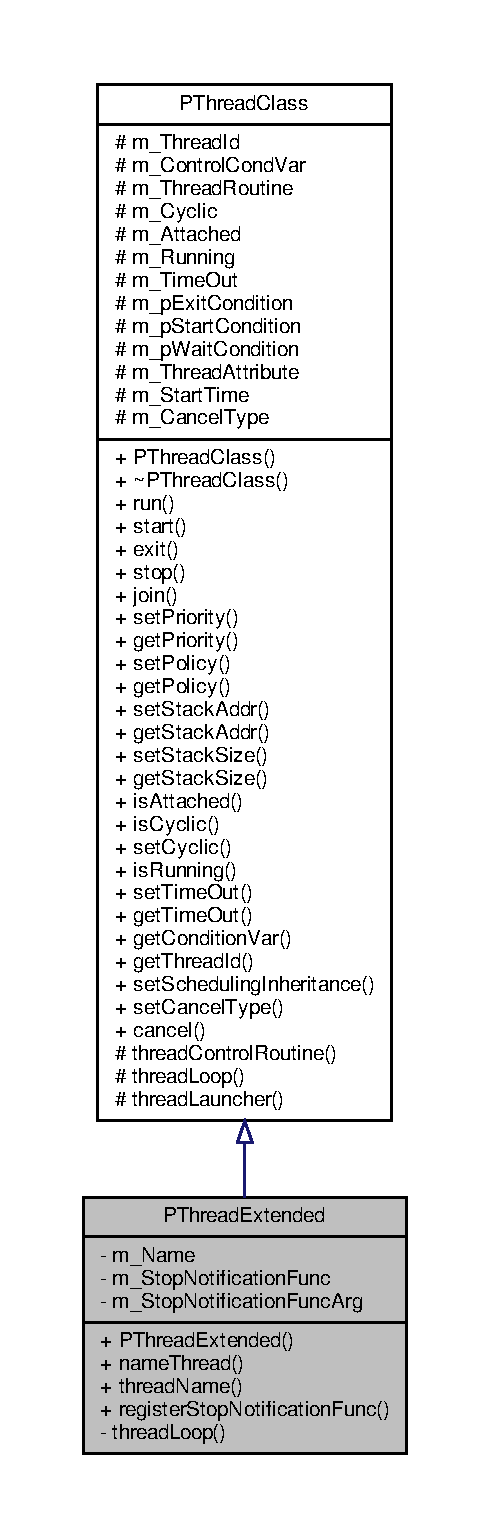
\includegraphics[height=550pt]{classPThreadExtended__inherit__graph}
\end{center}
\end{figure}
\subsection*{Public Member Functions}
\begin{DoxyCompactItemize}
\item 
\hyperlink{classPThreadExtended_a7bbc8901875c01e475b7a1637e176cad}{P\+Thread\+Extended} (\hyperlink{structRunnable}{Runnable} Routine, unsigned long Time=\hyperlink{PThreadClassLib_8h_a9d2d74d73cb5d069fbfcbcfebf42bd6e}{P\+T\+H\+R\+E\+A\+D\+\_\+\+I\+N\+F\+I\+N\+I\+TE}, bool Cyclic\+Thread=false, bool Attached\+Thread=true)
\item 
void \hyperlink{classPThreadExtended_a1df3e69e3cfae6f56e12da3ce80446d4}{name\+Thread} (string Name)
\item 
string \hyperlink{classPThreadExtended_a3c49f906e273860f45c44b5a988cf139}{thread\+Name} ()
\item 
void \hyperlink{classPThreadExtended_aa9a16de484a20e787223ee8750e6d7c1}{register\+Stop\+Notification\+Func} (\hyperlink{group__FUNC__DEFS_ga164076b53d35e4dba4c51bb336c15dab}{P\+Thread\+Notification\+Func\+Type} Func, void $\ast$Arg)
\end{DoxyCompactItemize}
\subsection*{Private Member Functions}
\begin{DoxyCompactItemize}
\item 
virtual void $\ast$ \hyperlink{classPThreadExtended_a43d31ca653ffe314e400a48a77f8e0a9}{thread\+Loop} ()
\begin{DoxyCompactList}\small\item\em Stop notification function argument. \end{DoxyCompactList}\end{DoxyCompactItemize}
\subsection*{Private Attributes}
\begin{DoxyCompactItemize}
\item 
string \hyperlink{classPThreadExtended_a43d72651db43fda0d627e87ca2a71ba3}{m\+\_\+\+Name}
\item 
\hyperlink{group__FUNC__DEFS_ga164076b53d35e4dba4c51bb336c15dab}{P\+Thread\+Notification\+Func\+Type} \hyperlink{classPThreadExtended_ae922e8bf6a63ea08521785c1875e02e2}{m\+\_\+\+Stop\+Notification\+Func}
\begin{DoxyCompactList}\small\item\em Thread name. \end{DoxyCompactList}\item 
void $\ast$ \hyperlink{classPThreadExtended_a666cf4f4189eb9dc04b2aa42da0f4acd}{m\+\_\+\+Stop\+Notification\+Func\+Arg}
\begin{DoxyCompactList}\small\item\em Stop notification function pointer. \end{DoxyCompactList}\end{DoxyCompactItemize}
\subsection*{Additional Inherited Members}


\subsection{Detailed Description}
P\+O\+S\+IX thread class with extended info

Wrapper on \hyperlink{classPThreadClass}{P\+Thread\+Class}. 

\subsection{Constructor \& Destructor Documentation}
\mbox{\Hypertarget{classPThreadExtended_a7bbc8901875c01e475b7a1637e176cad}\label{classPThreadExtended_a7bbc8901875c01e475b7a1637e176cad}} 
\index{P\+Thread\+Extended@{P\+Thread\+Extended}!P\+Thread\+Extended@{P\+Thread\+Extended}}
\index{P\+Thread\+Extended@{P\+Thread\+Extended}!P\+Thread\+Extended@{P\+Thread\+Extended}}
\subsubsection{\texorpdfstring{P\+Thread\+Extended()}{PThreadExtended()}}
{\footnotesize\ttfamily P\+Thread\+Extended\+::\+P\+Thread\+Extended (\begin{DoxyParamCaption}\item[{\hyperlink{structRunnable}{Runnable}}]{Routine,  }\item[{unsigned long}]{Time = {\ttfamily \hyperlink{PThreadClassLib_8h_a9d2d74d73cb5d069fbfcbcfebf42bd6e}{P\+T\+H\+R\+E\+A\+D\+\_\+\+I\+N\+F\+I\+N\+I\+TE}},  }\item[{bool}]{Cyclic\+Thread = {\ttfamily false},  }\item[{bool}]{Attached\+Thread = {\ttfamily true} }\end{DoxyParamCaption})\hspace{0.3cm}{\ttfamily [inline]}}

Constructor 
\begin{DoxyParams}{Parameters}
{\em Routine} & \+: routines structure reference. \\
\hline
{\em Time} & \+: cyclic period value in milliseconds. \\
\hline
{\em Cyclic\+Thread} & \+: cyclic (true) or one-\/shot (false) thread. \\
\hline
{\em Attached\+Thread} & \+: attached (true) or unattached (false) thread. \\
\hline
{\em Bound\+Thread} & \+: binding to L\+WP flag. Applicable only on supporting binding O\+Ss. \\
\hline
\end{DoxyParams}

\begin{DoxyExceptions}{Exceptions}
{\em \hyperlink{classThreadException}{Thread\+Exception}} & \\
\hline
\end{DoxyExceptions}


\subsection{Member Function Documentation}
\mbox{\Hypertarget{classPThreadExtended_a1df3e69e3cfae6f56e12da3ce80446d4}\label{classPThreadExtended_a1df3e69e3cfae6f56e12da3ce80446d4}} 
\index{P\+Thread\+Extended@{P\+Thread\+Extended}!name\+Thread@{name\+Thread}}
\index{name\+Thread@{name\+Thread}!P\+Thread\+Extended@{P\+Thread\+Extended}}
\subsubsection{\texorpdfstring{name\+Thread()}{nameThread()}}
{\footnotesize\ttfamily void P\+Thread\+Extended\+::name\+Thread (\begin{DoxyParamCaption}\item[{string}]{Name }\end{DoxyParamCaption})\hspace{0.3cm}{\ttfamily [inline]}}

Name the thread. 
\begin{DoxyParams}{Parameters}
{\em Name} & \+: thread name string. \\
\hline
\end{DoxyParams}
\mbox{\Hypertarget{classPThreadExtended_aa9a16de484a20e787223ee8750e6d7c1}\label{classPThreadExtended_aa9a16de484a20e787223ee8750e6d7c1}} 
\index{P\+Thread\+Extended@{P\+Thread\+Extended}!register\+Stop\+Notification\+Func@{register\+Stop\+Notification\+Func}}
\index{register\+Stop\+Notification\+Func@{register\+Stop\+Notification\+Func}!P\+Thread\+Extended@{P\+Thread\+Extended}}
\subsubsection{\texorpdfstring{register\+Stop\+Notification\+Func()}{registerStopNotificationFunc()}}
{\footnotesize\ttfamily void P\+Thread\+Extended\+::register\+Stop\+Notification\+Func (\begin{DoxyParamCaption}\item[{\hyperlink{group__FUNC__DEFS_ga164076b53d35e4dba4c51bb336c15dab}{P\+Thread\+Notification\+Func\+Type}}]{Func,  }\item[{void $\ast$}]{Arg }\end{DoxyParamCaption})\hspace{0.3cm}{\ttfamily [inline]}}

Registering of thread notification function. ~\newline
 The function is actually called on main thread context, therefore should be as short as possible in runtime. 
\begin{DoxyParams}{Parameters}
{\em Func} & \+: notification function pointer. \\
\hline
{\em Arg} & \+: notification function argument. \\
\hline
\end{DoxyParams}
\mbox{\Hypertarget{classPThreadExtended_a43d31ca653ffe314e400a48a77f8e0a9}\label{classPThreadExtended_a43d31ca653ffe314e400a48a77f8e0a9}} 
\index{P\+Thread\+Extended@{P\+Thread\+Extended}!thread\+Loop@{thread\+Loop}}
\index{thread\+Loop@{thread\+Loop}!P\+Thread\+Extended@{P\+Thread\+Extended}}
\subsubsection{\texorpdfstring{thread\+Loop()}{threadLoop()}}
{\footnotesize\ttfamily void $\ast$ P\+Thread\+Extended\+::thread\+Loop (\begin{DoxyParamCaption}{ }\end{DoxyParamCaption})\hspace{0.3cm}{\ttfamily [private]}, {\ttfamily [virtual]}}



Stop notification function argument. 

Internal thread loop. 

Reimplemented from \hyperlink{classPThreadClass_a77732762f14058291d35bdbbc49018c6}{P\+Thread\+Class}.

\mbox{\Hypertarget{classPThreadExtended_a3c49f906e273860f45c44b5a988cf139}\label{classPThreadExtended_a3c49f906e273860f45c44b5a988cf139}} 
\index{P\+Thread\+Extended@{P\+Thread\+Extended}!thread\+Name@{thread\+Name}}
\index{thread\+Name@{thread\+Name}!P\+Thread\+Extended@{P\+Thread\+Extended}}
\subsubsection{\texorpdfstring{thread\+Name()}{threadName()}}
{\footnotesize\ttfamily string P\+Thread\+Extended\+::thread\+Name (\begin{DoxyParamCaption}{ }\end{DoxyParamCaption})\hspace{0.3cm}{\ttfamily [inline]}}

Get thread name. \begin{DoxyReturn}{Returns}
Thread name string. 
\end{DoxyReturn}


\subsection{Member Data Documentation}
\mbox{\Hypertarget{classPThreadExtended_a43d72651db43fda0d627e87ca2a71ba3}\label{classPThreadExtended_a43d72651db43fda0d627e87ca2a71ba3}} 
\index{P\+Thread\+Extended@{P\+Thread\+Extended}!m\+\_\+\+Name@{m\+\_\+\+Name}}
\index{m\+\_\+\+Name@{m\+\_\+\+Name}!P\+Thread\+Extended@{P\+Thread\+Extended}}
\subsubsection{\texorpdfstring{m\+\_\+\+Name}{m\_Name}}
{\footnotesize\ttfamily string P\+Thread\+Extended\+::m\+\_\+\+Name\hspace{0.3cm}{\ttfamily [private]}}

\mbox{\Hypertarget{classPThreadExtended_ae922e8bf6a63ea08521785c1875e02e2}\label{classPThreadExtended_ae922e8bf6a63ea08521785c1875e02e2}} 
\index{P\+Thread\+Extended@{P\+Thread\+Extended}!m\+\_\+\+Stop\+Notification\+Func@{m\+\_\+\+Stop\+Notification\+Func}}
\index{m\+\_\+\+Stop\+Notification\+Func@{m\+\_\+\+Stop\+Notification\+Func}!P\+Thread\+Extended@{P\+Thread\+Extended}}
\subsubsection{\texorpdfstring{m\+\_\+\+Stop\+Notification\+Func}{m\_StopNotificationFunc}}
{\footnotesize\ttfamily \hyperlink{group__FUNC__DEFS_ga164076b53d35e4dba4c51bb336c15dab}{P\+Thread\+Notification\+Func\+Type} P\+Thread\+Extended\+::m\+\_\+\+Stop\+Notification\+Func\hspace{0.3cm}{\ttfamily [private]}}



Thread name. 

\mbox{\Hypertarget{classPThreadExtended_a666cf4f4189eb9dc04b2aa42da0f4acd}\label{classPThreadExtended_a666cf4f4189eb9dc04b2aa42da0f4acd}} 
\index{P\+Thread\+Extended@{P\+Thread\+Extended}!m\+\_\+\+Stop\+Notification\+Func\+Arg@{m\+\_\+\+Stop\+Notification\+Func\+Arg}}
\index{m\+\_\+\+Stop\+Notification\+Func\+Arg@{m\+\_\+\+Stop\+Notification\+Func\+Arg}!P\+Thread\+Extended@{P\+Thread\+Extended}}
\subsubsection{\texorpdfstring{m\+\_\+\+Stop\+Notification\+Func\+Arg}{m\_StopNotificationFuncArg}}
{\footnotesize\ttfamily void$\ast$ P\+Thread\+Extended\+::m\+\_\+\+Stop\+Notification\+Func\+Arg\hspace{0.3cm}{\ttfamily [private]}}



Stop notification function pointer. 



The documentation for this class was generated from the following files\+:\begin{DoxyCompactItemize}
\item 
\hyperlink{PThreadExtended_8h}{P\+Thread\+Extended.\+h}\item 
\hyperlink{PThreadExtended_8cpp}{P\+Thread\+Extended.\+cpp}\end{DoxyCompactItemize}

\hypertarget{structRunnable}{}\section{Runnable Struct Reference}
\label{structRunnable}\index{Runnable@{Runnable}}


{\ttfamily \#include $<$P\+Thread\+Class.\+h$>$}

\subsection*{Public Member Functions}
\begin{DoxyCompactItemize}
\item 
\hyperlink{structRunnable_a55a54a10b0f3733f276d07db584f2549}{Runnable} (\hyperlink{group__FUNC__DEFS_gaeef66643e734485d781ca826339879ea}{P\+Thread\+Routine\+Type} p\+Routine, \hyperlink{group__FUNC__DEFS_ga77ca9e695666040451b77632df4847b9}{P\+Thread\+Clean\+Up\+Routine\+Type} p\+Clean\+Up\+Routine=N\+U\+LL, void $\ast$p=N\+U\+LL, void $\ast$cp=N\+U\+LL, int Clean\+Up\+Execute=0)
\item 
\hyperlink{structRunnable_ad4a6cf9daf0f17048c0a8972e90d295d}{operator P\+Thread\+Routine\+Type} ()
\begin{DoxyCompactList}\small\item\em Cast to thread routine operator. \end{DoxyCompactList}\item 
\hyperlink{structRunnable_a8d99767578589e79ba59f8ddece80e69}{operator P\+Thread\+Clean\+Up\+Routine\+Type} ()
\begin{DoxyCompactList}\small\item\em Cast to clean-\/up routine operator. \end{DoxyCompactList}\item 
void $\ast$ \hyperlink{structRunnable_a017eeb87c9076ffcb34338bba7fefb99}{operator()} ()
\begin{DoxyCompactList}\small\item\em Function operator. \end{DoxyCompactList}\end{DoxyCompactItemize}
\subsection*{Public Attributes}
\begin{DoxyCompactItemize}
\item 
\hyperlink{group__FUNC__DEFS_gaeef66643e734485d781ca826339879ea}{P\+Thread\+Routine\+Type} \hyperlink{structRunnable_ad850dfe862b73a3e9f59c5fe383bd20d}{pthread\+Routine}
\begin{DoxyCompactList}\small\item\em Thread routine. \end{DoxyCompactList}\item 
\hyperlink{group__FUNC__DEFS_ga77ca9e695666040451b77632df4847b9}{P\+Thread\+Clean\+Up\+Routine\+Type} \hyperlink{structRunnable_a62c14bef1f2acabcff9c126faf9c0218}{clean\+Up\+Routine}
\begin{DoxyCompactList}\small\item\em Clean-\/up routine. \end{DoxyCompactList}\item 
void $\ast$ \hyperlink{structRunnable_a5b950239feca1d3033297fae933209e9}{p\+Context}
\begin{DoxyCompactList}\small\item\em Thread routine context. \end{DoxyCompactList}\item 
void $\ast$ \hyperlink{structRunnable_a30fc8274b7103f58fbbd56aa165692b4}{p\+Clean\+Up\+Context}
\begin{DoxyCompactList}\small\item\em Clean-\/up routine context. \end{DoxyCompactList}\item 
int \hyperlink{structRunnable_aee103a0bc58c7dc4a92da67eac8436fc}{m\+\_\+\+Clean\+Up\+Execute}
\begin{DoxyCompactList}\small\item\em Clean-\/up handler execution flag. \end{DoxyCompactList}\end{DoxyCompactItemize}


\subsection{Detailed Description}
C++ wrapper on thread routine and clean-\/up routine. 

\subsection{Constructor \& Destructor Documentation}
\mbox{\Hypertarget{structRunnable_a55a54a10b0f3733f276d07db584f2549}\label{structRunnable_a55a54a10b0f3733f276d07db584f2549}} 
\index{Runnable@{Runnable}!Runnable@{Runnable}}
\index{Runnable@{Runnable}!Runnable@{Runnable}}
\subsubsection{\texorpdfstring{Runnable()}{Runnable()}}
{\footnotesize\ttfamily Runnable\+::\+Runnable (\begin{DoxyParamCaption}\item[{\hyperlink{group__FUNC__DEFS_gaeef66643e734485d781ca826339879ea}{P\+Thread\+Routine\+Type}}]{p\+Routine,  }\item[{\hyperlink{group__FUNC__DEFS_ga77ca9e695666040451b77632df4847b9}{P\+Thread\+Clean\+Up\+Routine\+Type}}]{p\+Clean\+Up\+Routine = {\ttfamily NULL},  }\item[{void $\ast$}]{p = {\ttfamily NULL},  }\item[{void $\ast$}]{cp = {\ttfamily NULL},  }\item[{int}]{Clean\+Up\+Execute = {\ttfamily 0} }\end{DoxyParamCaption})\hspace{0.3cm}{\ttfamily [inline]}}

Constructor 
\begin{DoxyParams}{Parameters}
{\em p\+Routine} & \+: pointer to thread routine. \\
\hline
{\em p\+Clean\+Up\+Routine} & \+: pointer to clean-\/up routine. \\
\hline
{\em p} & \+: pointer to thread routine context. \\
\hline
{\em cp} & \+: pointer to clean-\/up routine context. \\
\hline
{\em Clean\+Up\+Execute} & \+: clean-\/up handler execution flag. \\
\hline
\end{DoxyParams}


\subsection{Member Function Documentation}
\mbox{\Hypertarget{structRunnable_a8d99767578589e79ba59f8ddece80e69}\label{structRunnable_a8d99767578589e79ba59f8ddece80e69}} 
\index{Runnable@{Runnable}!operator P\+Thread\+Clean\+Up\+Routine\+Type@{operator P\+Thread\+Clean\+Up\+Routine\+Type}}
\index{operator P\+Thread\+Clean\+Up\+Routine\+Type@{operator P\+Thread\+Clean\+Up\+Routine\+Type}!Runnable@{Runnable}}
\subsubsection{\texorpdfstring{operator P\+Thread\+Clean\+Up\+Routine\+Type()}{operator PThreadCleanUpRoutineType()}}
{\footnotesize\ttfamily Runnable\+::operator \hyperlink{group__FUNC__DEFS_ga77ca9e695666040451b77632df4847b9}{P\+Thread\+Clean\+Up\+Routine\+Type} (\begin{DoxyParamCaption}{ }\end{DoxyParamCaption})\hspace{0.3cm}{\ttfamily [inline]}}



Cast to clean-\/up routine operator. 

\mbox{\Hypertarget{structRunnable_ad4a6cf9daf0f17048c0a8972e90d295d}\label{structRunnable_ad4a6cf9daf0f17048c0a8972e90d295d}} 
\index{Runnable@{Runnable}!operator P\+Thread\+Routine\+Type@{operator P\+Thread\+Routine\+Type}}
\index{operator P\+Thread\+Routine\+Type@{operator P\+Thread\+Routine\+Type}!Runnable@{Runnable}}
\subsubsection{\texorpdfstring{operator P\+Thread\+Routine\+Type()}{operator PThreadRoutineType()}}
{\footnotesize\ttfamily Runnable\+::operator \hyperlink{group__FUNC__DEFS_gaeef66643e734485d781ca826339879ea}{P\+Thread\+Routine\+Type} (\begin{DoxyParamCaption}{ }\end{DoxyParamCaption})\hspace{0.3cm}{\ttfamily [inline]}}



Cast to thread routine operator. 

\mbox{\Hypertarget{structRunnable_a017eeb87c9076ffcb34338bba7fefb99}\label{structRunnable_a017eeb87c9076ffcb34338bba7fefb99}} 
\index{Runnable@{Runnable}!operator()@{operator()}}
\index{operator()@{operator()}!Runnable@{Runnable}}
\subsubsection{\texorpdfstring{operator()()}{operator()()}}
{\footnotesize\ttfamily void$\ast$ Runnable\+::operator() (\begin{DoxyParamCaption}{ }\end{DoxyParamCaption})\hspace{0.3cm}{\ttfamily [inline]}}



Function operator. 



\subsection{Member Data Documentation}
\mbox{\Hypertarget{structRunnable_a62c14bef1f2acabcff9c126faf9c0218}\label{structRunnable_a62c14bef1f2acabcff9c126faf9c0218}} 
\index{Runnable@{Runnable}!clean\+Up\+Routine@{clean\+Up\+Routine}}
\index{clean\+Up\+Routine@{clean\+Up\+Routine}!Runnable@{Runnable}}
\subsubsection{\texorpdfstring{clean\+Up\+Routine}{cleanUpRoutine}}
{\footnotesize\ttfamily \hyperlink{group__FUNC__DEFS_ga77ca9e695666040451b77632df4847b9}{P\+Thread\+Clean\+Up\+Routine\+Type} Runnable\+::clean\+Up\+Routine}



Clean-\/up routine. 

\mbox{\Hypertarget{structRunnable_aee103a0bc58c7dc4a92da67eac8436fc}\label{structRunnable_aee103a0bc58c7dc4a92da67eac8436fc}} 
\index{Runnable@{Runnable}!m\+\_\+\+Clean\+Up\+Execute@{m\+\_\+\+Clean\+Up\+Execute}}
\index{m\+\_\+\+Clean\+Up\+Execute@{m\+\_\+\+Clean\+Up\+Execute}!Runnable@{Runnable}}
\subsubsection{\texorpdfstring{m\+\_\+\+Clean\+Up\+Execute}{m\_CleanUpExecute}}
{\footnotesize\ttfamily int Runnable\+::m\+\_\+\+Clean\+Up\+Execute}



Clean-\/up handler execution flag. 

\mbox{\Hypertarget{structRunnable_a30fc8274b7103f58fbbd56aa165692b4}\label{structRunnable_a30fc8274b7103f58fbbd56aa165692b4}} 
\index{Runnable@{Runnable}!p\+Clean\+Up\+Context@{p\+Clean\+Up\+Context}}
\index{p\+Clean\+Up\+Context@{p\+Clean\+Up\+Context}!Runnable@{Runnable}}
\subsubsection{\texorpdfstring{p\+Clean\+Up\+Context}{pCleanUpContext}}
{\footnotesize\ttfamily void$\ast$ Runnable\+::p\+Clean\+Up\+Context}



Clean-\/up routine context. 

\mbox{\Hypertarget{structRunnable_a5b950239feca1d3033297fae933209e9}\label{structRunnable_a5b950239feca1d3033297fae933209e9}} 
\index{Runnable@{Runnable}!p\+Context@{p\+Context}}
\index{p\+Context@{p\+Context}!Runnable@{Runnable}}
\subsubsection{\texorpdfstring{p\+Context}{pContext}}
{\footnotesize\ttfamily void$\ast$ Runnable\+::p\+Context}



Thread routine context. 

\mbox{\Hypertarget{structRunnable_ad850dfe862b73a3e9f59c5fe383bd20d}\label{structRunnable_ad850dfe862b73a3e9f59c5fe383bd20d}} 
\index{Runnable@{Runnable}!pthread\+Routine@{pthread\+Routine}}
\index{pthread\+Routine@{pthread\+Routine}!Runnable@{Runnable}}
\subsubsection{\texorpdfstring{pthread\+Routine}{pthreadRoutine}}
{\footnotesize\ttfamily \hyperlink{group__FUNC__DEFS_gaeef66643e734485d781ca826339879ea}{P\+Thread\+Routine\+Type} Runnable\+::pthread\+Routine}



Thread routine. 



The documentation for this struct was generated from the following file\+:\begin{DoxyCompactItemize}
\item 
\hyperlink{PThreadClass_8h}{P\+Thread\+Class.\+h}\end{DoxyCompactItemize}

\hypertarget{classSpecificCondition}{}\section{Specific\+Condition Class Reference}
\label{classSpecificCondition}\index{Specific\+Condition@{Specific\+Condition}}


{\ttfamily \#include $<$Cond\+Var\+Class.\+h$>$}

\subsection*{Public Member Functions}
\begin{DoxyCompactItemize}
\item 
\hyperlink{classSpecificCondition_aeaad30c2483d565580a0c5def33a56bf}{Specific\+Condition} (\hyperlink{classCondVarClass}{Cond\+Var\+Class} \&Cond, \hyperlink{classCondVarClass_a8e27f99972b8b95f064d6657a4583a5b}{Cond\+Var\+Class\+::\+Predicate\+Id\+Type} Index) noexcept(false)
\item 
bool \hyperlink{classSpecificCondition_a136588886dab164bdb5ef1cbca9bd222}{get\+Predicate} () noexcept(false)
\item 
void \hyperlink{classSpecificCondition_ae339d4e8b0e0944887d6e81f284f834e}{set\+Predicate} (bool Predicate\+Value) noexcept(false)
\item 
int \hyperlink{classSpecificCondition_aac09e84b11482d7651a7001a6a0757cd}{lock\+Mutex} ()
\item 
int \hyperlink{classSpecificCondition_a408f84395e536d0e9ae0604e7ac3feb1}{try\+Lock\+Mutex} ()
\item 
int \hyperlink{classSpecificCondition_a8cdac09a54f900329b35a54349cbba44}{unlock\+Mutex} ()
\item 
int \hyperlink{classSpecificCondition_a8af0e884bb8b3d765b5a59761efdec04}{signal} ()
\item 
int \hyperlink{classSpecificCondition_a74ec8602bf6bc6de21faee0fb6910c2d}{broadcast} ()
\item 
int \hyperlink{classSpecificCondition_a56b9eb97c2713b979b54ce05534ff5c4}{wait} (time\+\_\+t Timeout=\hyperlink{PThreadClassLib_8h_a9d2d74d73cb5d069fbfcbcfebf42bd6e}{P\+T\+H\+R\+E\+A\+D\+\_\+\+I\+N\+F\+I\+N\+I\+TE})
\end{DoxyCompactItemize}
\subsection*{Protected Attributes}
\begin{DoxyCompactItemize}
\item 
\hyperlink{classCondVarClass}{Cond\+Var\+Class} \& \hyperlink{classSpecificCondition_af686c95919169acecede46f1821e1660}{m\+\_\+\+Cond\+Var\+Cl}
\begin{DoxyCompactList}\small\item\em Condition variable object reference. \end{DoxyCompactList}\item 
\hyperlink{classCondVarClass_a8e27f99972b8b95f064d6657a4583a5b}{Cond\+Var\+Class\+::\+Predicate\+Id\+Type} \hyperlink{classSpecificCondition_a9de96adba4d7b9347d2ae60a49b57d9b}{m\+\_\+\+Index}
\begin{DoxyCompactList}\small\item\em Specified predicate number. \end{DoxyCompactList}\end{DoxyCompactItemize}


\subsection{Detailed Description}
Wrapper on specific predicate of conditopn variable. 

\subsection{Constructor \& Destructor Documentation}
\mbox{\Hypertarget{classSpecificCondition_aeaad30c2483d565580a0c5def33a56bf}\label{classSpecificCondition_aeaad30c2483d565580a0c5def33a56bf}} 
\index{Specific\+Condition@{Specific\+Condition}!Specific\+Condition@{Specific\+Condition}}
\index{Specific\+Condition@{Specific\+Condition}!Specific\+Condition@{Specific\+Condition}}
\subsubsection{\texorpdfstring{Specific\+Condition()}{SpecificCondition()}}
{\footnotesize\ttfamily Specific\+Condition\+::\+Specific\+Condition (\begin{DoxyParamCaption}\item[{\hyperlink{classCondVarClass}{Cond\+Var\+Class} \&}]{Cond,  }\item[{\hyperlink{classCondVarClass_a8e27f99972b8b95f064d6657a4583a5b}{Cond\+Var\+Class\+::\+Predicate\+Id\+Type}}]{Index }\end{DoxyParamCaption})\hspace{0.3cm}{\ttfamily [noexcept]}}

Constructor 
\begin{DoxyParams}{Parameters}
{\em Cond} & \+: condition variable object reference. \\
\hline
{\em Index} & \+: number of specific predicate. \\
\hline
\end{DoxyParams}


\subsection{Member Function Documentation}
\mbox{\Hypertarget{classSpecificCondition_a74ec8602bf6bc6de21faee0fb6910c2d}\label{classSpecificCondition_a74ec8602bf6bc6de21faee0fb6910c2d}} 
\index{Specific\+Condition@{Specific\+Condition}!broadcast@{broadcast}}
\index{broadcast@{broadcast}!Specific\+Condition@{Specific\+Condition}}
\subsubsection{\texorpdfstring{broadcast()}{broadcast()}}
{\footnotesize\ttfamily int Specific\+Condition\+::broadcast (\begin{DoxyParamCaption}{ }\end{DoxyParamCaption})\hspace{0.3cm}{\ttfamily [inline]}}

Broadcast condition variable. \begin{DoxyReturn}{Returns}
result of broadcast operation (0 -\/ success). 
\end{DoxyReturn}
\mbox{\Hypertarget{classSpecificCondition_a136588886dab164bdb5ef1cbca9bd222}\label{classSpecificCondition_a136588886dab164bdb5ef1cbca9bd222}} 
\index{Specific\+Condition@{Specific\+Condition}!get\+Predicate@{get\+Predicate}}
\index{get\+Predicate@{get\+Predicate}!Specific\+Condition@{Specific\+Condition}}
\subsubsection{\texorpdfstring{get\+Predicate()}{getPredicate()}}
{\footnotesize\ttfamily bool Specific\+Condition\+::get\+Predicate (\begin{DoxyParamCaption}{ }\end{DoxyParamCaption})\hspace{0.3cm}{\ttfamily [inline]}, {\ttfamily [noexcept]}}

Get value of the specified predicate. \begin{DoxyReturn}{Returns}
Predicate value. 
\end{DoxyReturn}

\begin{DoxyExceptions}{Exceptions}
{\em \hyperlink{classThreadException}{Thread\+Exception}} & \\
\hline
\end{DoxyExceptions}
\mbox{\Hypertarget{classSpecificCondition_aac09e84b11482d7651a7001a6a0757cd}\label{classSpecificCondition_aac09e84b11482d7651a7001a6a0757cd}} 
\index{Specific\+Condition@{Specific\+Condition}!lock\+Mutex@{lock\+Mutex}}
\index{lock\+Mutex@{lock\+Mutex}!Specific\+Condition@{Specific\+Condition}}
\subsubsection{\texorpdfstring{lock\+Mutex()}{lockMutex()}}
{\footnotesize\ttfamily int Specific\+Condition\+::lock\+Mutex (\begin{DoxyParamCaption}{ }\end{DoxyParamCaption})\hspace{0.3cm}{\ttfamily [inline]}}

Lock condition variable associated mutual exclusive lock. \begin{DoxyReturn}{Returns}
result of lock operation (0 -\/ success). 
\end{DoxyReturn}
\mbox{\Hypertarget{classSpecificCondition_ae339d4e8b0e0944887d6e81f284f834e}\label{classSpecificCondition_ae339d4e8b0e0944887d6e81f284f834e}} 
\index{Specific\+Condition@{Specific\+Condition}!set\+Predicate@{set\+Predicate}}
\index{set\+Predicate@{set\+Predicate}!Specific\+Condition@{Specific\+Condition}}
\subsubsection{\texorpdfstring{set\+Predicate()}{setPredicate()}}
{\footnotesize\ttfamily void Specific\+Condition\+::set\+Predicate (\begin{DoxyParamCaption}\item[{bool}]{Predicate\+Value }\end{DoxyParamCaption})\hspace{0.3cm}{\ttfamily [inline]}, {\ttfamily [noexcept]}}

Set value of the specified predicate. 
\begin{DoxyParams}{Parameters}
{\em Predicate\+Value} & \+: predicate value. \\
\hline
\end{DoxyParams}

\begin{DoxyExceptions}{Exceptions}
{\em \hyperlink{classThreadException}{Thread\+Exception}} & \\
\hline
\end{DoxyExceptions}
\mbox{\Hypertarget{classSpecificCondition_a8af0e884bb8b3d765b5a59761efdec04}\label{classSpecificCondition_a8af0e884bb8b3d765b5a59761efdec04}} 
\index{Specific\+Condition@{Specific\+Condition}!signal@{signal}}
\index{signal@{signal}!Specific\+Condition@{Specific\+Condition}}
\subsubsection{\texorpdfstring{signal()}{signal()}}
{\footnotesize\ttfamily int Specific\+Condition\+::signal (\begin{DoxyParamCaption}{ }\end{DoxyParamCaption})\hspace{0.3cm}{\ttfamily [inline]}}

Signal condition variable . \begin{DoxyReturn}{Returns}
result of signal operation (0 -\/ success). 
\end{DoxyReturn}
\mbox{\Hypertarget{classSpecificCondition_a408f84395e536d0e9ae0604e7ac3feb1}\label{classSpecificCondition_a408f84395e536d0e9ae0604e7ac3feb1}} 
\index{Specific\+Condition@{Specific\+Condition}!try\+Lock\+Mutex@{try\+Lock\+Mutex}}
\index{try\+Lock\+Mutex@{try\+Lock\+Mutex}!Specific\+Condition@{Specific\+Condition}}
\subsubsection{\texorpdfstring{try\+Lock\+Mutex()}{tryLockMutex()}}
{\footnotesize\ttfamily int Specific\+Condition\+::try\+Lock\+Mutex (\begin{DoxyParamCaption}{ }\end{DoxyParamCaption})\hspace{0.3cm}{\ttfamily [inline]}}

Try to lock condition variable associated mutual exclusive lock. \begin{DoxyReturn}{Returns}
result of lock operation (0 -\/ success). 
\end{DoxyReturn}
\mbox{\Hypertarget{classSpecificCondition_a8cdac09a54f900329b35a54349cbba44}\label{classSpecificCondition_a8cdac09a54f900329b35a54349cbba44}} 
\index{Specific\+Condition@{Specific\+Condition}!unlock\+Mutex@{unlock\+Mutex}}
\index{unlock\+Mutex@{unlock\+Mutex}!Specific\+Condition@{Specific\+Condition}}
\subsubsection{\texorpdfstring{unlock\+Mutex()}{unlockMutex()}}
{\footnotesize\ttfamily int Specific\+Condition\+::unlock\+Mutex (\begin{DoxyParamCaption}{ }\end{DoxyParamCaption})\hspace{0.3cm}{\ttfamily [inline]}}

Unlock condition variable associated mutual exclusive lock. \begin{DoxyReturn}{Returns}
result of unlock operation (0 -\/ success). 
\end{DoxyReturn}
\mbox{\Hypertarget{classSpecificCondition_a56b9eb97c2713b979b54ce05534ff5c4}\label{classSpecificCondition_a56b9eb97c2713b979b54ce05534ff5c4}} 
\index{Specific\+Condition@{Specific\+Condition}!wait@{wait}}
\index{wait@{wait}!Specific\+Condition@{Specific\+Condition}}
\subsubsection{\texorpdfstring{wait()}{wait()}}
{\footnotesize\ttfamily int Specific\+Condition\+::wait (\begin{DoxyParamCaption}\item[{time\+\_\+t}]{Timeout = {\ttfamily \hyperlink{PThreadClassLib_8h_a9d2d74d73cb5d069fbfcbcfebf42bd6e}{P\+T\+H\+R\+E\+A\+D\+\_\+\+I\+N\+F\+I\+N\+I\+TE}} }\end{DoxyParamCaption})\hspace{0.3cm}{\ttfamily [inline]}}

Wait for condition variable to be signaled. \begin{DoxyReturn}{Returns}
result of wait \+: ~\newline
 0 -\/ condition variable is signaled.~\newline
 E\+T\+I\+M\+E\+D\+O\+UT -\/ wait timeout expired.~\newline
 other -\/ error.~\newline
 
\end{DoxyReturn}


\subsection{Member Data Documentation}
\mbox{\Hypertarget{classSpecificCondition_af686c95919169acecede46f1821e1660}\label{classSpecificCondition_af686c95919169acecede46f1821e1660}} 
\index{Specific\+Condition@{Specific\+Condition}!m\+\_\+\+Cond\+Var\+Cl@{m\+\_\+\+Cond\+Var\+Cl}}
\index{m\+\_\+\+Cond\+Var\+Cl@{m\+\_\+\+Cond\+Var\+Cl}!Specific\+Condition@{Specific\+Condition}}
\subsubsection{\texorpdfstring{m\+\_\+\+Cond\+Var\+Cl}{m\_CondVarCl}}
{\footnotesize\ttfamily \hyperlink{classCondVarClass}{Cond\+Var\+Class}\& Specific\+Condition\+::m\+\_\+\+Cond\+Var\+Cl\hspace{0.3cm}{\ttfamily [protected]}}



Condition variable object reference. 

\mbox{\Hypertarget{classSpecificCondition_a9de96adba4d7b9347d2ae60a49b57d9b}\label{classSpecificCondition_a9de96adba4d7b9347d2ae60a49b57d9b}} 
\index{Specific\+Condition@{Specific\+Condition}!m\+\_\+\+Index@{m\+\_\+\+Index}}
\index{m\+\_\+\+Index@{m\+\_\+\+Index}!Specific\+Condition@{Specific\+Condition}}
\subsubsection{\texorpdfstring{m\+\_\+\+Index}{m\_Index}}
{\footnotesize\ttfamily \hyperlink{classCondVarClass_a8e27f99972b8b95f064d6657a4583a5b}{Cond\+Var\+Class\+::\+Predicate\+Id\+Type} Specific\+Condition\+::m\+\_\+\+Index\hspace{0.3cm}{\ttfamily [protected]}}



Specified predicate number. 



The documentation for this class was generated from the following files\+:\begin{DoxyCompactItemize}
\item 
\hyperlink{CondVarClass_8h}{Cond\+Var\+Class.\+h}\item 
\hyperlink{CondVarClass_8cpp}{Cond\+Var\+Class.\+cpp}\end{DoxyCompactItemize}

\hypertarget{classThreadException}{}\section{Thread\+Exception Class Reference}
\label{classThreadException}\index{Thread\+Exception@{Thread\+Exception}}


{\ttfamily \#include $<$Thread\+Exception.\+h$>$}



Inheritance diagram for Thread\+Exception\+:\nopagebreak
\begin{figure}[H]
\begin{center}
\leavevmode
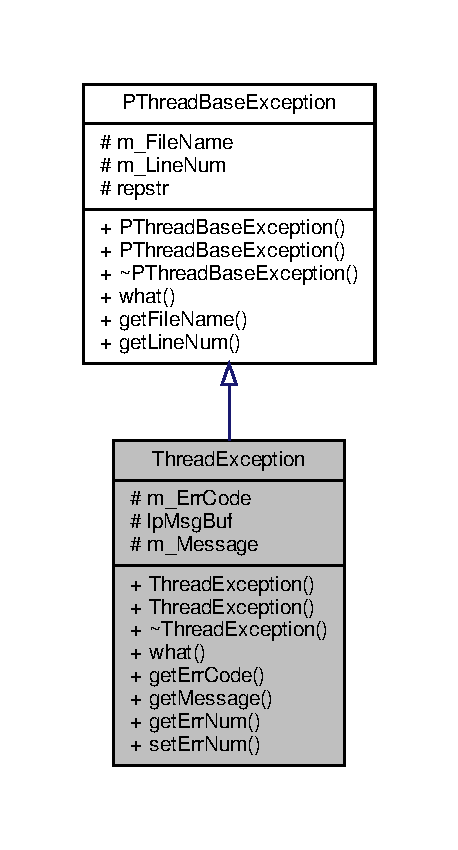
\includegraphics[width=220pt]{classThreadException__inherit__graph}
\end{center}
\end{figure}
\subsection*{Public Member Functions}
\begin{DoxyCompactItemize}
\item 
\hyperlink{classThreadException_a6367b52f02d9b964073474e2a4bf065a}{Thread\+Exception} (const char $\ast$File\+Name, int Line\+Num, int errcode)
\item 
\hyperlink{classThreadException_a8e2fd5fddc16b2ef79f9ff9152e07bae}{Thread\+Exception} (const char $\ast$File\+Name, int Line\+Num, const char $\ast$Message)
\item 
virtual \hyperlink{classThreadException_a2b6c29bbca2d87808a573530f9bf354c}{$\sim$\+Thread\+Exception} ()  throw ()
\item 
virtual const char $\ast$ \hyperlink{classThreadException_a3b8dcf8e441a9cba0539ca2455087e57}{what} ()
\item 
int \hyperlink{classThreadException_adb548dbb352870603d20921ffe5d2535}{get\+Err\+Code} ()
\item 
char $\ast$ \hyperlink{classThreadException_a49a3a8d894925c4f76b0ec3338354006}{get\+Message} ()
\item 
int \hyperlink{classThreadException_a03564289d24e7d5246bf43fbcae2f7f3}{get\+Err\+Num} ()
\item 
void \hyperlink{classThreadException_adaa1940a2b6fa8beff808bee9b9fa2cf}{set\+Err\+Num} (int Num=0)
\end{DoxyCompactItemize}
\subsection*{Protected Attributes}
\begin{DoxyCompactItemize}
\item 
int \hyperlink{classThreadException_af35c621f09ff63e9928a8ad5ce596d34}{m\+\_\+\+Err\+Code}
\begin{DoxyCompactList}\small\item\em Error code. \end{DoxyCompactList}\item 
char \hyperlink{classThreadException_a7687b9835112b0381c09ac0b52637be1}{lp\+Msg\+Buf} \mbox{[}256\mbox{]}
\begin{DoxyCompactList}\small\item\em Error message buffer. \end{DoxyCompactList}\item 
char \hyperlink{classThreadException_aa2ab3078b7211738d8eeb1e9e4e2a8cb}{m\+\_\+\+Message} \mbox{[}256\mbox{]}
\begin{DoxyCompactList}\small\item\em User\+Message buffer. \end{DoxyCompactList}\end{DoxyCompactItemize}


\subsection{Detailed Description}
Thread class library exception. 

\subsection{Constructor \& Destructor Documentation}
\mbox{\Hypertarget{classThreadException_a6367b52f02d9b964073474e2a4bf065a}\label{classThreadException_a6367b52f02d9b964073474e2a4bf065a}} 
\index{Thread\+Exception@{Thread\+Exception}!Thread\+Exception@{Thread\+Exception}}
\index{Thread\+Exception@{Thread\+Exception}!Thread\+Exception@{Thread\+Exception}}
\subsubsection{\texorpdfstring{Thread\+Exception()}{ThreadException()}\hspace{0.1cm}{\footnotesize\ttfamily [1/2]}}
{\footnotesize\ttfamily Thread\+Exception\+::\+Thread\+Exception (\begin{DoxyParamCaption}\item[{const char $\ast$}]{File\+Name,  }\item[{int}]{Line\+Num,  }\item[{int}]{errcode }\end{DoxyParamCaption})}

Constructor

Constructs exception object with filename and line number. 
\begin{DoxyParams}{Parameters}
{\em File\+Name} & \+: name of source file. \\
\hline
{\em Line\+Num} & \+: number of code line. \\
\hline
{\em errcode} & \+: error numeric code. \\
\hline
\end{DoxyParams}
\mbox{\Hypertarget{classThreadException_a8e2fd5fddc16b2ef79f9ff9152e07bae}\label{classThreadException_a8e2fd5fddc16b2ef79f9ff9152e07bae}} 
\index{Thread\+Exception@{Thread\+Exception}!Thread\+Exception@{Thread\+Exception}}
\index{Thread\+Exception@{Thread\+Exception}!Thread\+Exception@{Thread\+Exception}}
\subsubsection{\texorpdfstring{Thread\+Exception()}{ThreadException()}\hspace{0.1cm}{\footnotesize\ttfamily [2/2]}}
{\footnotesize\ttfamily Thread\+Exception\+::\+Thread\+Exception (\begin{DoxyParamCaption}\item[{const char $\ast$}]{File\+Name,  }\item[{int}]{Line\+Num,  }\item[{const char $\ast$}]{Message }\end{DoxyParamCaption})}

Constructor

Constructs exception object with filename, line number and text message 
\begin{DoxyParams}{Parameters}
{\em File\+Name} & \+: name of source file. \\
\hline
{\em Line\+Num} & \+: number of code line. \\
\hline
{\em Message} & \+: user message. \\
\hline
\end{DoxyParams}
\mbox{\Hypertarget{classThreadException_a2b6c29bbca2d87808a573530f9bf354c}\label{classThreadException_a2b6c29bbca2d87808a573530f9bf354c}} 
\index{Thread\+Exception@{Thread\+Exception}!````~Thread\+Exception@{$\sim$\+Thread\+Exception}}
\index{````~Thread\+Exception@{$\sim$\+Thread\+Exception}!Thread\+Exception@{Thread\+Exception}}
\subsubsection{\texorpdfstring{$\sim$\+Thread\+Exception()}{~ThreadException()}}
{\footnotesize\ttfamily virtual Thread\+Exception\+::$\sim$\+Thread\+Exception (\begin{DoxyParamCaption}{ }\end{DoxyParamCaption}) throw  ) \hspace{0.3cm}{\ttfamily [inline]}, {\ttfamily [virtual]}}

Destructor

Intentionally empty 

\subsection{Member Function Documentation}
\mbox{\Hypertarget{classThreadException_adb548dbb352870603d20921ffe5d2535}\label{classThreadException_adb548dbb352870603d20921ffe5d2535}} 
\index{Thread\+Exception@{Thread\+Exception}!get\+Err\+Code@{get\+Err\+Code}}
\index{get\+Err\+Code@{get\+Err\+Code}!Thread\+Exception@{Thread\+Exception}}
\subsubsection{\texorpdfstring{get\+Err\+Code()}{getErrCode()}}
{\footnotesize\ttfamily int Thread\+Exception\+::get\+Err\+Code (\begin{DoxyParamCaption}{ }\end{DoxyParamCaption})\hspace{0.3cm}{\ttfamily [inline]}}

Delivers error code \begin{DoxyReturn}{Returns}
error cod of the exception cause. 
\end{DoxyReturn}
\mbox{\Hypertarget{classThreadException_a03564289d24e7d5246bf43fbcae2f7f3}\label{classThreadException_a03564289d24e7d5246bf43fbcae2f7f3}} 
\index{Thread\+Exception@{Thread\+Exception}!get\+Err\+Num@{get\+Err\+Num}}
\index{get\+Err\+Num@{get\+Err\+Num}!Thread\+Exception@{Thread\+Exception}}
\subsubsection{\texorpdfstring{get\+Err\+Num()}{getErrNum()}}
{\footnotesize\ttfamily int Thread\+Exception\+::get\+Err\+Num (\begin{DoxyParamCaption}{ }\end{DoxyParamCaption})\hspace{0.3cm}{\ttfamily [inline]}}

Delivers errno \begin{DoxyReturn}{Returns}
errno 
\end{DoxyReturn}
\mbox{\Hypertarget{classThreadException_a49a3a8d894925c4f76b0ec3338354006}\label{classThreadException_a49a3a8d894925c4f76b0ec3338354006}} 
\index{Thread\+Exception@{Thread\+Exception}!get\+Message@{get\+Message}}
\index{get\+Message@{get\+Message}!Thread\+Exception@{Thread\+Exception}}
\subsubsection{\texorpdfstring{get\+Message()}{getMessage()}}
{\footnotesize\ttfamily char$\ast$ Thread\+Exception\+::get\+Message (\begin{DoxyParamCaption}{ }\end{DoxyParamCaption})\hspace{0.3cm}{\ttfamily [inline]}}

Delivers error message. \begin{DoxyReturn}{Returns}
message buffer. 
\end{DoxyReturn}
\mbox{\Hypertarget{classThreadException_adaa1940a2b6fa8beff808bee9b9fa2cf}\label{classThreadException_adaa1940a2b6fa8beff808bee9b9fa2cf}} 
\index{Thread\+Exception@{Thread\+Exception}!set\+Err\+Num@{set\+Err\+Num}}
\index{set\+Err\+Num@{set\+Err\+Num}!Thread\+Exception@{Thread\+Exception}}
\subsubsection{\texorpdfstring{set\+Err\+Num()}{setErrNum()}}
{\footnotesize\ttfamily void Thread\+Exception\+::set\+Err\+Num (\begin{DoxyParamCaption}\item[{int}]{Num = {\ttfamily 0} }\end{DoxyParamCaption})\hspace{0.3cm}{\ttfamily [inline]}}

Sets error number. 
\begin{DoxyParams}{Parameters}
{\em Num} & \+: error number. \\
\hline
\end{DoxyParams}
\mbox{\Hypertarget{classThreadException_a3b8dcf8e441a9cba0539ca2455087e57}\label{classThreadException_a3b8dcf8e441a9cba0539ca2455087e57}} 
\index{Thread\+Exception@{Thread\+Exception}!what@{what}}
\index{what@{what}!Thread\+Exception@{Thread\+Exception}}
\subsubsection{\texorpdfstring{what()}{what()}}
{\footnotesize\ttfamily const char $\ast$ Thread\+Exception\+::what (\begin{DoxyParamCaption}{ }\end{DoxyParamCaption})\hspace{0.3cm}{\ttfamily [virtual]}}

Reports exception\textquotesingle{}s properties. \begin{DoxyReturn}{Returns}
String buffer with report text. 
\end{DoxyReturn}


Reimplemented from \hyperlink{group__EXCEPT__GROUP_ga4389169c01caec3fe93ac45a5d69a9ec}{P\+Thread\+Base\+Exception}.



\subsection{Member Data Documentation}
\mbox{\Hypertarget{classThreadException_a7687b9835112b0381c09ac0b52637be1}\label{classThreadException_a7687b9835112b0381c09ac0b52637be1}} 
\index{Thread\+Exception@{Thread\+Exception}!lp\+Msg\+Buf@{lp\+Msg\+Buf}}
\index{lp\+Msg\+Buf@{lp\+Msg\+Buf}!Thread\+Exception@{Thread\+Exception}}
\subsubsection{\texorpdfstring{lp\+Msg\+Buf}{lpMsgBuf}}
{\footnotesize\ttfamily char Thread\+Exception\+::lp\+Msg\+Buf\mbox{[}256\mbox{]}\hspace{0.3cm}{\ttfamily [protected]}}



Error message buffer. 

\mbox{\Hypertarget{classThreadException_af35c621f09ff63e9928a8ad5ce596d34}\label{classThreadException_af35c621f09ff63e9928a8ad5ce596d34}} 
\index{Thread\+Exception@{Thread\+Exception}!m\+\_\+\+Err\+Code@{m\+\_\+\+Err\+Code}}
\index{m\+\_\+\+Err\+Code@{m\+\_\+\+Err\+Code}!Thread\+Exception@{Thread\+Exception}}
\subsubsection{\texorpdfstring{m\+\_\+\+Err\+Code}{m\_ErrCode}}
{\footnotesize\ttfamily int Thread\+Exception\+::m\+\_\+\+Err\+Code\hspace{0.3cm}{\ttfamily [protected]}}



Error code. 

\mbox{\Hypertarget{classThreadException_aa2ab3078b7211738d8eeb1e9e4e2a8cb}\label{classThreadException_aa2ab3078b7211738d8eeb1e9e4e2a8cb}} 
\index{Thread\+Exception@{Thread\+Exception}!m\+\_\+\+Message@{m\+\_\+\+Message}}
\index{m\+\_\+\+Message@{m\+\_\+\+Message}!Thread\+Exception@{Thread\+Exception}}
\subsubsection{\texorpdfstring{m\+\_\+\+Message}{m\_Message}}
{\footnotesize\ttfamily char Thread\+Exception\+::m\+\_\+\+Message\mbox{[}256\mbox{]}\hspace{0.3cm}{\ttfamily [protected]}}



User\+Message buffer. 



The documentation for this class was generated from the following files\+:\begin{DoxyCompactItemize}
\item 
\hyperlink{ThreadException_8h}{Thread\+Exception.\+h}\item 
\hyperlink{ThreadException_8cpp}{Thread\+Exception.\+cpp}\end{DoxyCompactItemize}

\hypertarget{structPThreadClassLib_1_1VersionTriple}{}\section{P\+Thread\+Class\+Lib\+:\+:Version\+Triple Struct Reference}
\label{structPThreadClassLib_1_1VersionTriple}\index{P\+Thread\+Class\+Lib\+::\+Version\+Triple@{P\+Thread\+Class\+Lib\+::\+Version\+Triple}}


Structure for library versions.  




{\ttfamily \#include $<$P\+Thread\+Class\+Lib.\+h$>$}

\subsection*{Public Attributes}
\begin{DoxyCompactItemize}
\item 
int \hyperlink{structPThreadClassLib_1_1VersionTriple_ab34a8a6d82b1b4cc6dd3e2e515a3176f}{Major}
\begin{DoxyCompactList}\small\item\em Major version number. \end{DoxyCompactList}\item 
int \hyperlink{structPThreadClassLib_1_1VersionTriple_ad937fe83d89788c30241f937bb8ddb37}{Minor}
\begin{DoxyCompactList}\small\item\em Minor version number. \end{DoxyCompactList}\item 
int \hyperlink{structPThreadClassLib_1_1VersionTriple_a51341849d79f4a8077291a4502fb4840}{Sub\+Minor}
\begin{DoxyCompactList}\small\item\em Minor subversion number. \end{DoxyCompactList}\end{DoxyCompactItemize}


\subsection{Detailed Description}
Structure for library versions. 

\subsection{Member Data Documentation}
\mbox{\Hypertarget{structPThreadClassLib_1_1VersionTriple_ab34a8a6d82b1b4cc6dd3e2e515a3176f}\label{structPThreadClassLib_1_1VersionTriple_ab34a8a6d82b1b4cc6dd3e2e515a3176f}} 
\index{P\+Thread\+Class\+Lib\+::\+Version\+Triple@{P\+Thread\+Class\+Lib\+::\+Version\+Triple}!Major@{Major}}
\index{Major@{Major}!P\+Thread\+Class\+Lib\+::\+Version\+Triple@{P\+Thread\+Class\+Lib\+::\+Version\+Triple}}
\subsubsection{\texorpdfstring{Major}{Major}}
{\footnotesize\ttfamily int P\+Thread\+Class\+Lib\+::\+Version\+Triple\+::\+Major}



Major version number. 

\mbox{\Hypertarget{structPThreadClassLib_1_1VersionTriple_ad937fe83d89788c30241f937bb8ddb37}\label{structPThreadClassLib_1_1VersionTriple_ad937fe83d89788c30241f937bb8ddb37}} 
\index{P\+Thread\+Class\+Lib\+::\+Version\+Triple@{P\+Thread\+Class\+Lib\+::\+Version\+Triple}!Minor@{Minor}}
\index{Minor@{Minor}!P\+Thread\+Class\+Lib\+::\+Version\+Triple@{P\+Thread\+Class\+Lib\+::\+Version\+Triple}}
\subsubsection{\texorpdfstring{Minor}{Minor}}
{\footnotesize\ttfamily int P\+Thread\+Class\+Lib\+::\+Version\+Triple\+::\+Minor}



Minor version number. 

\mbox{\Hypertarget{structPThreadClassLib_1_1VersionTriple_a51341849d79f4a8077291a4502fb4840}\label{structPThreadClassLib_1_1VersionTriple_a51341849d79f4a8077291a4502fb4840}} 
\index{P\+Thread\+Class\+Lib\+::\+Version\+Triple@{P\+Thread\+Class\+Lib\+::\+Version\+Triple}!Sub\+Minor@{Sub\+Minor}}
\index{Sub\+Minor@{Sub\+Minor}!P\+Thread\+Class\+Lib\+::\+Version\+Triple@{P\+Thread\+Class\+Lib\+::\+Version\+Triple}}
\subsubsection{\texorpdfstring{Sub\+Minor}{SubMinor}}
{\footnotesize\ttfamily int P\+Thread\+Class\+Lib\+::\+Version\+Triple\+::\+Sub\+Minor}



Minor subversion number. 



The documentation for this struct was generated from the following file\+:\begin{DoxyCompactItemize}
\item 
\hyperlink{PThreadClassLib_8h}{P\+Thread\+Class\+Lib.\+h}\end{DoxyCompactItemize}

\chapter{File Documentation}
\hypertarget{CondVarClass_8cpp}{}\section{Cond\+Var\+Class.\+cpp File Reference}
\label{CondVarClass_8cpp}\index{Cond\+Var\+Class.\+cpp@{Cond\+Var\+Class.\+cpp}}
{\ttfamily \#include $<$Cond\+Var\+Class.\+h$>$}\newline
{\ttfamily \#include $<$time.\+h$>$}\newline
{\ttfamily \#include $<$sys/time.\+h$>$}\newline
Include dependency graph for Cond\+Var\+Class.\+cpp\+:\nopagebreak
\begin{figure}[H]
\begin{center}
\leavevmode
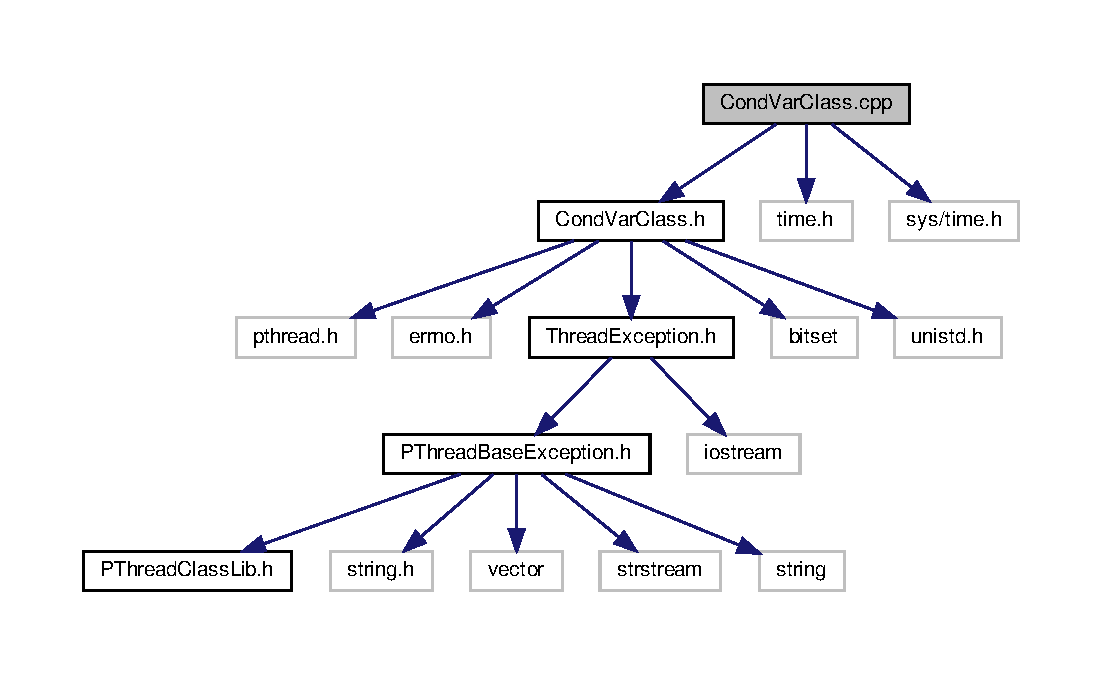
\includegraphics[width=350pt]{CondVarClass_8cpp__incl}
\end{center}
\end{figure}

\hypertarget{CondVarClass_8h}{}\section{Cond\+Var\+Class.\+h File Reference}
\label{CondVarClass_8h}\index{Cond\+Var\+Class.\+h@{Cond\+Var\+Class.\+h}}
{\ttfamily \#include $<$pthread.\+h$>$}\newline
{\ttfamily \#include $<$errno.\+h$>$}\newline
{\ttfamily \#include $<$Thread\+Exception.\+h$>$}\newline
{\ttfamily \#include $<$bitset$>$}\newline
{\ttfamily \#include $<$unistd.\+h$>$}\newline
Include dependency graph for Cond\+Var\+Class.\+h\+:\nopagebreak
\begin{figure}[H]
\begin{center}
\leavevmode
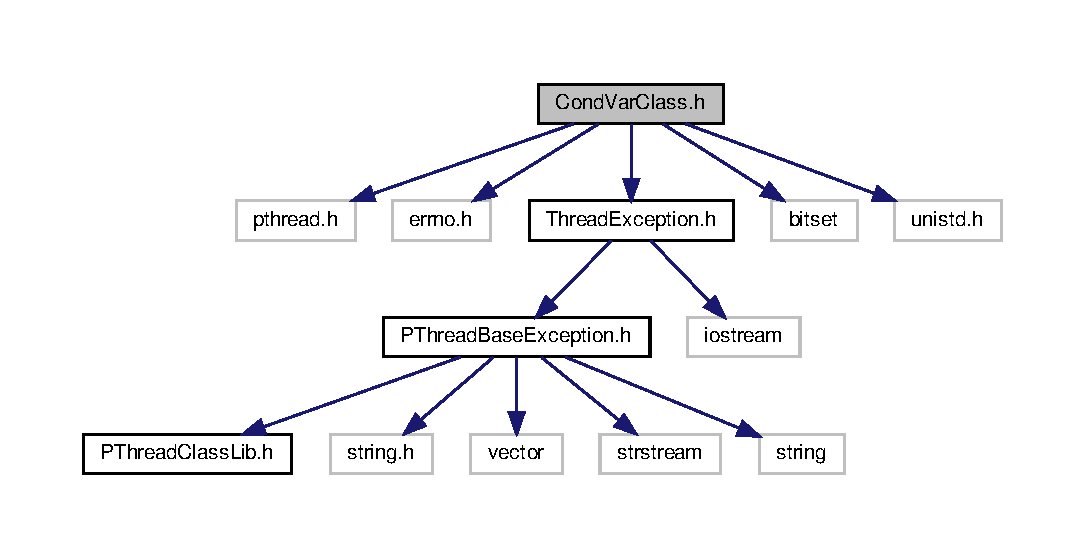
\includegraphics[width=350pt]{CondVarClass_8h__incl}
\end{center}
\end{figure}
This graph shows which files directly or indirectly include this file\+:\nopagebreak
\begin{figure}[H]
\begin{center}
\leavevmode
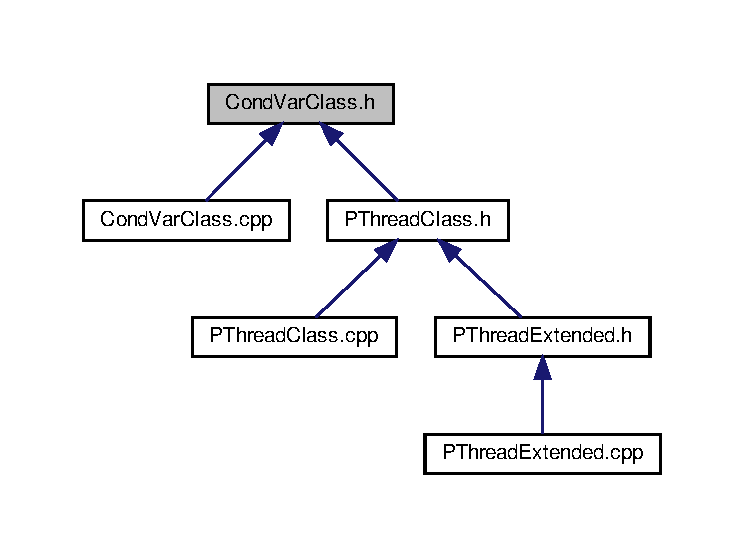
\includegraphics[width=350pt]{CondVarClass_8h__dep__incl}
\end{center}
\end{figure}
\subsection*{Classes}
\begin{DoxyCompactItemize}
\item 
class \hyperlink{classCondVarClass}{Cond\+Var\+Class}
\item 
class \hyperlink{classSpecificCondition}{Specific\+Condition}
\end{DoxyCompactItemize}
\subsection*{Macros}
\begin{DoxyCompactItemize}
\item 
\#define \hyperlink{CondVarClass_8h_a6e8562f77c7eeea17bbd7dad99cc5a5d}{M\+A\+X\+\_\+\+N\+U\+M\+\_\+\+O\+F\+\_\+\+P\+R\+E\+DS}~32
\end{DoxyCompactItemize}


\subsection{Macro Definition Documentation}
\mbox{\Hypertarget{CondVarClass_8h_a6e8562f77c7eeea17bbd7dad99cc5a5d}\label{CondVarClass_8h_a6e8562f77c7eeea17bbd7dad99cc5a5d}} 
\index{Cond\+Var\+Class.\+h@{Cond\+Var\+Class.\+h}!M\+A\+X\+\_\+\+N\+U\+M\+\_\+\+O\+F\+\_\+\+P\+R\+E\+DS@{M\+A\+X\+\_\+\+N\+U\+M\+\_\+\+O\+F\+\_\+\+P\+R\+E\+DS}}
\index{M\+A\+X\+\_\+\+N\+U\+M\+\_\+\+O\+F\+\_\+\+P\+R\+E\+DS@{M\+A\+X\+\_\+\+N\+U\+M\+\_\+\+O\+F\+\_\+\+P\+R\+E\+DS}!Cond\+Var\+Class.\+h@{Cond\+Var\+Class.\+h}}
\subsubsection{\texorpdfstring{M\+A\+X\+\_\+\+N\+U\+M\+\_\+\+O\+F\+\_\+\+P\+R\+E\+DS}{MAX\_NUM\_OF\_PREDS}}
{\footnotesize\ttfamily \#define M\+A\+X\+\_\+\+N\+U\+M\+\_\+\+O\+F\+\_\+\+P\+R\+E\+DS~32}






\hypertarget{PBarrierClass_8cpp}{}\section{P\+Barrier\+Class.\+cpp File Reference}
\label{PBarrierClass_8cpp}\index{P\+Barrier\+Class.\+cpp@{P\+Barrier\+Class.\+cpp}}
{\ttfamily \#include $<$P\+Barrier\+Class.\+h$>$}\newline
Include dependency graph for P\+Barrier\+Class.\+cpp\+:\nopagebreak
\begin{figure}[H]
\begin{center}
\leavevmode
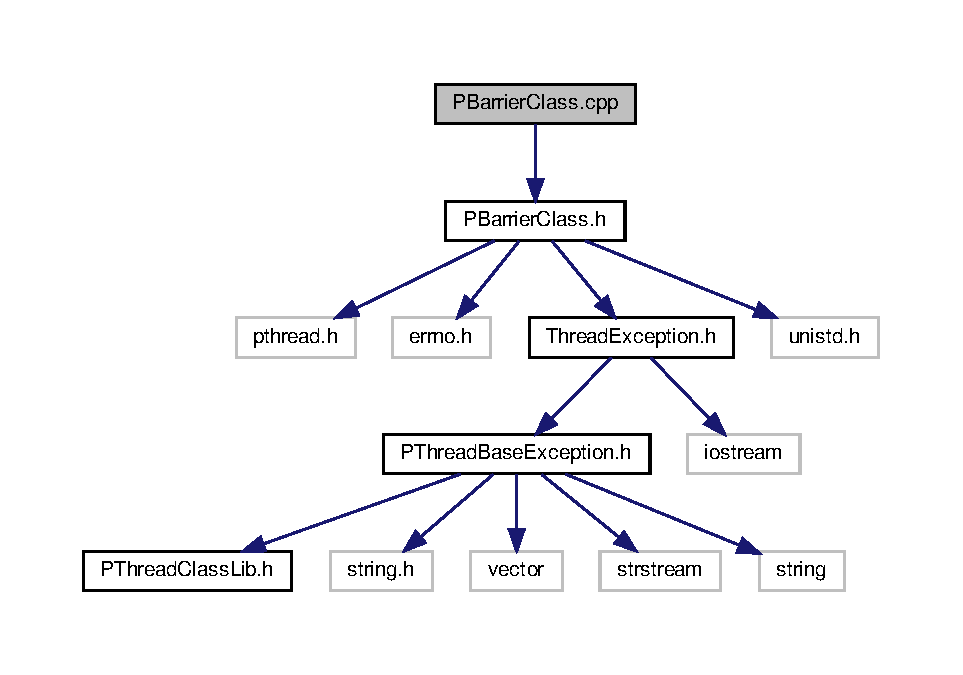
\includegraphics[width=350pt]{PBarrierClass_8cpp__incl}
\end{center}
\end{figure}

\hypertarget{PBarrierClass_8h}{}\section{P\+Barrier\+Class.\+h File Reference}
\label{PBarrierClass_8h}\index{P\+Barrier\+Class.\+h@{P\+Barrier\+Class.\+h}}
{\ttfamily \#include $<$pthread.\+h$>$}\newline
{\ttfamily \#include $<$errno.\+h$>$}\newline
{\ttfamily \#include $<$Thread\+Exception.\+h$>$}\newline
{\ttfamily \#include $<$unistd.\+h$>$}\newline
Include dependency graph for P\+Barrier\+Class.\+h\+:\nopagebreak
\begin{figure}[H]
\begin{center}
\leavevmode
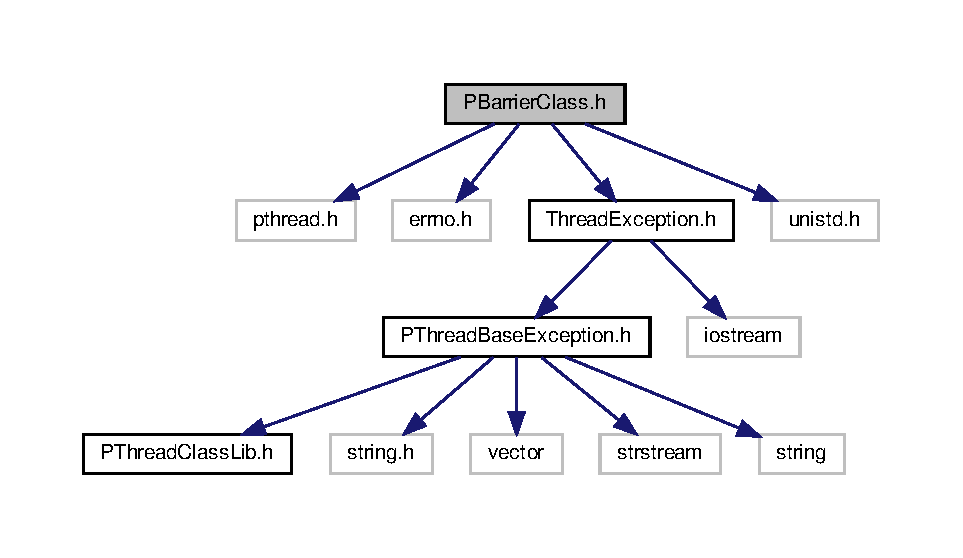
\includegraphics[width=350pt]{PBarrierClass_8h__incl}
\end{center}
\end{figure}
This graph shows which files directly or indirectly include this file\+:\nopagebreak
\begin{figure}[H]
\begin{center}
\leavevmode
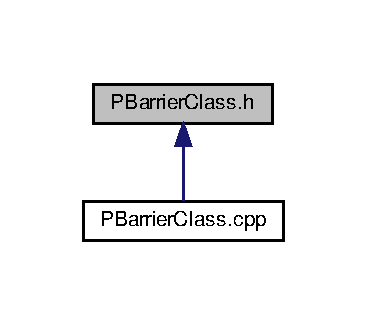
\includegraphics[width=176pt]{PBarrierClass_8h__dep__incl}
\end{center}
\end{figure}
\subsection*{Classes}
\begin{DoxyCompactItemize}
\item 
class \hyperlink{classPBarrierClass}{P\+Barrier\+Class}
\end{DoxyCompactItemize}

\hypertarget{PMutexClass_8cpp}{}\section{P\+Mutex\+Class.\+cpp File Reference}
\label{PMutexClass_8cpp}\index{P\+Mutex\+Class.\+cpp@{P\+Mutex\+Class.\+cpp}}
{\ttfamily \#include $<$P\+Mutex\+Class.\+h$>$}\newline
{\ttfamily \#include $<$time.\+h$>$}\newline
Include dependency graph for P\+Mutex\+Class.\+cpp\+:\nopagebreak
\begin{figure}[H]
\begin{center}
\leavevmode
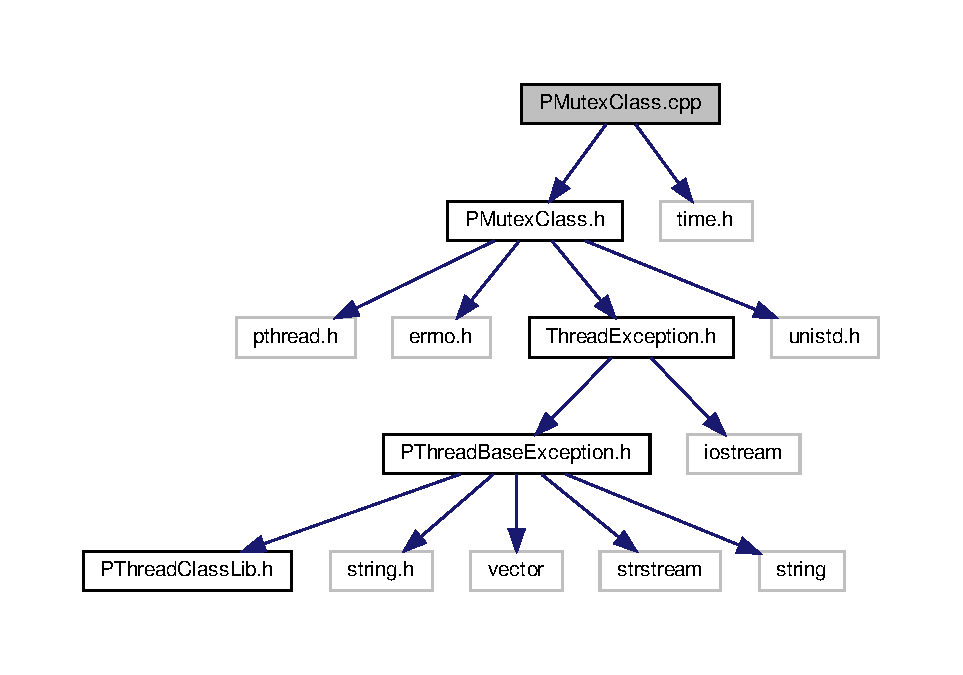
\includegraphics[width=350pt]{PMutexClass_8cpp__incl}
\end{center}
\end{figure}

\hypertarget{PMutexClass_8h}{}\section{P\+Mutex\+Class.\+h File Reference}
\label{PMutexClass_8h}\index{P\+Mutex\+Class.\+h@{P\+Mutex\+Class.\+h}}
{\ttfamily \#include $<$pthread.\+h$>$}\newline
{\ttfamily \#include $<$errno.\+h$>$}\newline
{\ttfamily \#include $<$Thread\+Exception.\+h$>$}\newline
{\ttfamily \#include $<$unistd.\+h$>$}\newline
Include dependency graph for P\+Mutex\+Class.\+h\+:\nopagebreak
\begin{figure}[H]
\begin{center}
\leavevmode
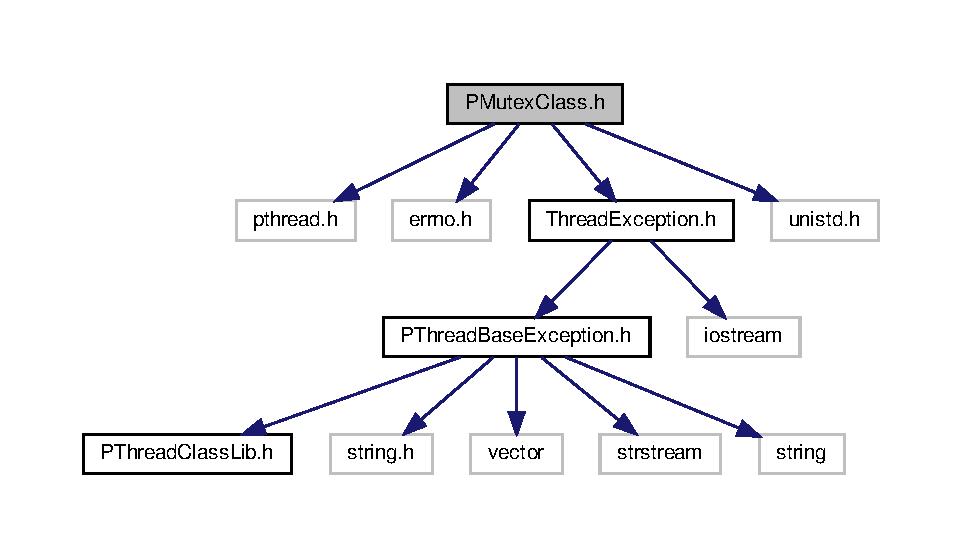
\includegraphics[width=350pt]{PMutexClass_8h__incl}
\end{center}
\end{figure}
This graph shows which files directly or indirectly include this file\+:\nopagebreak
\begin{figure}[H]
\begin{center}
\leavevmode
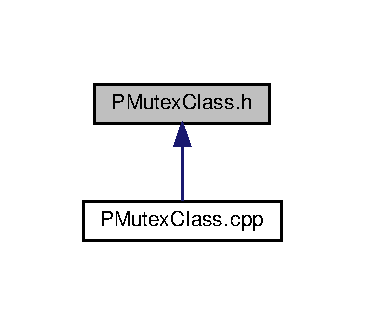
\includegraphics[width=175pt]{PMutexClass_8h__dep__incl}
\end{center}
\end{figure}
\subsection*{Classes}
\begin{DoxyCompactItemize}
\item 
class \hyperlink{classPMutexClass}{P\+Mutex\+Class}
\end{DoxyCompactItemize}

\hypertarget{PRWLockClass_8cpp}{}\section{P\+R\+W\+Lock\+Class.\+cpp File Reference}
\label{PRWLockClass_8cpp}\index{P\+R\+W\+Lock\+Class.\+cpp@{P\+R\+W\+Lock\+Class.\+cpp}}
{\ttfamily \#include $<$P\+R\+W\+Lock\+Class.\+h$>$}\newline
{\ttfamily \#include $<$time.\+h$>$}\newline
Include dependency graph for P\+R\+W\+Lock\+Class.\+cpp\+:\nopagebreak
\begin{figure}[H]
\begin{center}
\leavevmode
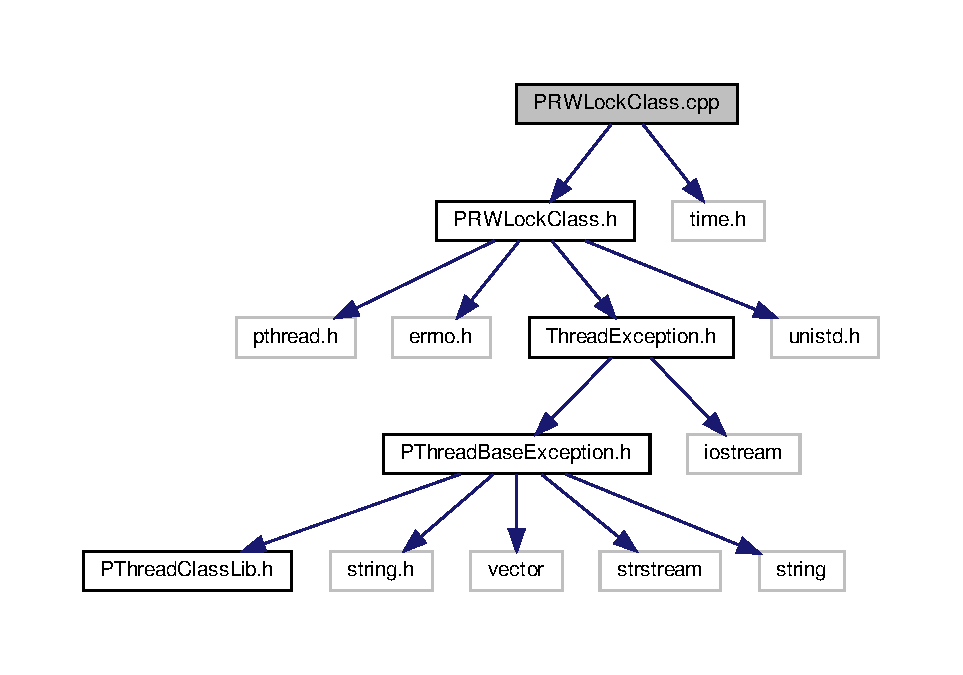
\includegraphics[width=350pt]{PRWLockClass_8cpp__incl}
\end{center}
\end{figure}

\hypertarget{PRWLockClass_8h}{}\section{P\+R\+W\+Lock\+Class.\+h File Reference}
\label{PRWLockClass_8h}\index{P\+R\+W\+Lock\+Class.\+h@{P\+R\+W\+Lock\+Class.\+h}}
{\ttfamily \#include $<$pthread.\+h$>$}\newline
{\ttfamily \#include $<$errno.\+h$>$}\newline
{\ttfamily \#include $<$Thread\+Exception.\+h$>$}\newline
{\ttfamily \#include $<$unistd.\+h$>$}\newline
Include dependency graph for P\+R\+W\+Lock\+Class.\+h\+:\nopagebreak
\begin{figure}[H]
\begin{center}
\leavevmode
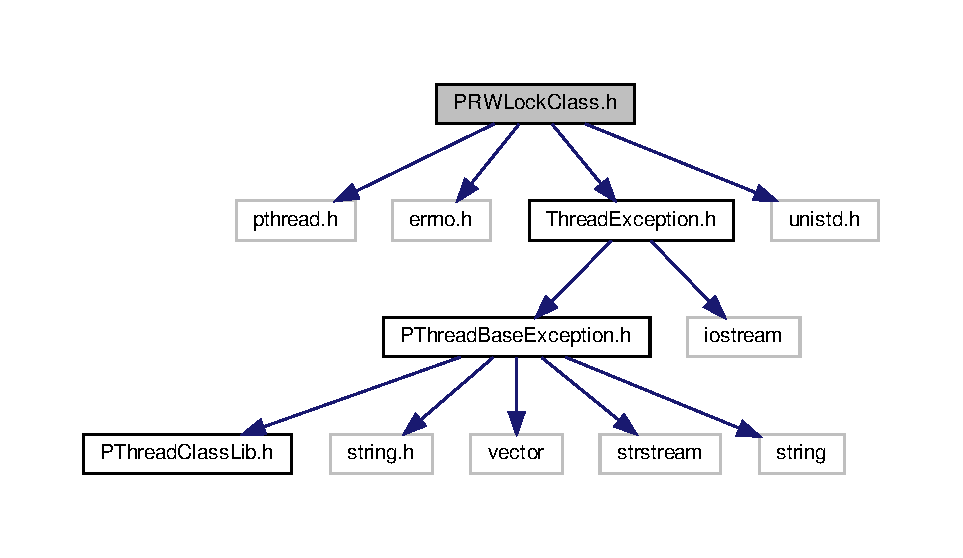
\includegraphics[width=350pt]{PRWLockClass_8h__incl}
\end{center}
\end{figure}
This graph shows which files directly or indirectly include this file\+:\nopagebreak
\begin{figure}[H]
\begin{center}
\leavevmode
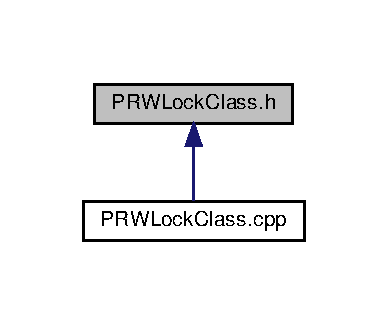
\includegraphics[width=186pt]{PRWLockClass_8h__dep__incl}
\end{center}
\end{figure}
\subsection*{Classes}
\begin{DoxyCompactItemize}
\item 
class \hyperlink{classPRWLockClass}{P\+R\+W\+Lock\+Class}
\end{DoxyCompactItemize}

\hypertarget{PThreadBaseException_8h}{}\section{P\+Thread\+Base\+Exception.\+h File Reference}
\label{PThreadBaseException_8h}\index{P\+Thread\+Base\+Exception.\+h@{P\+Thread\+Base\+Exception.\+h}}
{\ttfamily \#include $<$P\+Thread\+Class\+Lib.\+h$>$}\newline
{\ttfamily \#include $<$string.\+h$>$}\newline
{\ttfamily \#include $<$vector$>$}\newline
{\ttfamily \#include $<$strstream$>$}\newline
{\ttfamily \#include $<$string$>$}\newline
Include dependency graph for P\+Thread\+Base\+Exception.\+h\+:\nopagebreak
\begin{figure}[H]
\begin{center}
\leavevmode
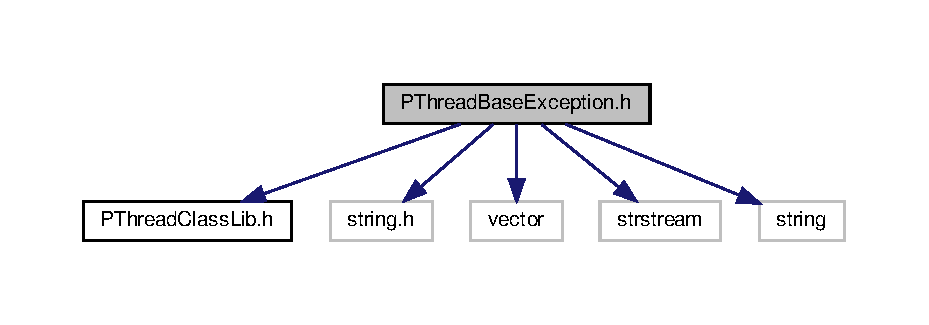
\includegraphics[width=350pt]{PThreadBaseException_8h__incl}
\end{center}
\end{figure}
This graph shows which files directly or indirectly include this file\+:\nopagebreak
\begin{figure}[H]
\begin{center}
\leavevmode
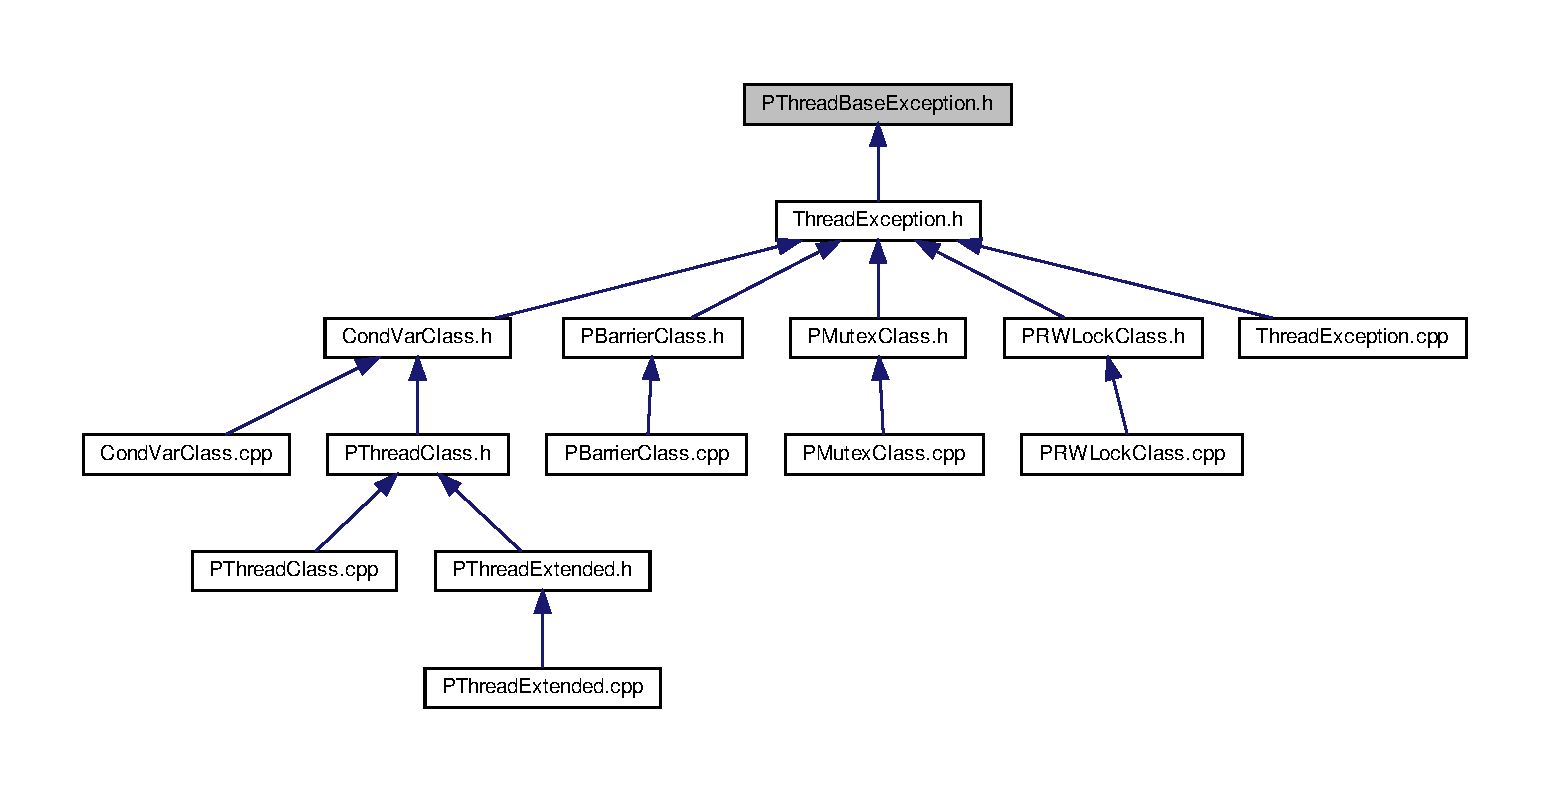
\includegraphics[width=350pt]{PThreadBaseException_8h__dep__incl}
\end{center}
\end{figure}
\subsection*{Classes}
\begin{DoxyCompactItemize}
\item 
class \hyperlink{classPThreadBaseException}{P\+Thread\+Base\+Exception}
\end{DoxyCompactItemize}
\subsection*{Macros}
\begin{DoxyCompactItemize}
\item 
\#define \hyperlink{PThreadBaseException_8h_adbba0f726fc66d7100916c683b7568ae}{G\+C\+C\+\_\+\+V\+E\+R\+S\+I\+ON}~(\+\_\+\+\_\+\+G\+N\+U\+C\+\_\+\+\_\+ $\ast$ 1000 + \+\_\+\+\_\+\+G\+N\+U\+C\+\_\+\+M\+I\+N\+O\+R\+\_\+\+\_\+)
\item 
\#define \hyperlink{PThreadBaseException_8h_a1a51a9063946272a0af9db0d88e3e363}{pthrrepstream}~strstream
\item 
\#define \hyperlink{group__EXCEPT__GROUP_gaf6a9cbd32371e5892a6b4190928651dd}{P\+T\+H\+R\+E\+A\+D\+\_\+\+E\+X\+C\+E\+P\+T\+I\+O\+N\+\_\+\+P\+A\+R\+A\+MS}~\+\_\+\+\_\+\+F\+I\+L\+E\+\_\+\+\_\+, \+\_\+\+\_\+\+L\+I\+N\+E\+\_\+\+\_\+
\begin{DoxyCompactList}\small\item\em Exception parameters includes filename and line number. \end{DoxyCompactList}\end{DoxyCompactItemize}


\subsection{Macro Definition Documentation}
\mbox{\Hypertarget{PThreadBaseException_8h_adbba0f726fc66d7100916c683b7568ae}\label{PThreadBaseException_8h_adbba0f726fc66d7100916c683b7568ae}} 
\index{P\+Thread\+Base\+Exception.\+h@{P\+Thread\+Base\+Exception.\+h}!G\+C\+C\+\_\+\+V\+E\+R\+S\+I\+ON@{G\+C\+C\+\_\+\+V\+E\+R\+S\+I\+ON}}
\index{G\+C\+C\+\_\+\+V\+E\+R\+S\+I\+ON@{G\+C\+C\+\_\+\+V\+E\+R\+S\+I\+ON}!P\+Thread\+Base\+Exception.\+h@{P\+Thread\+Base\+Exception.\+h}}
\subsubsection{\texorpdfstring{G\+C\+C\+\_\+\+V\+E\+R\+S\+I\+ON}{GCC\_VERSION}}
{\footnotesize\ttfamily \#define G\+C\+C\+\_\+\+V\+E\+R\+S\+I\+ON~(\+\_\+\+\_\+\+G\+N\+U\+C\+\_\+\+\_\+ $\ast$ 1000 + \+\_\+\+\_\+\+G\+N\+U\+C\+\_\+\+M\+I\+N\+O\+R\+\_\+\+\_\+)}

\mbox{\Hypertarget{PThreadBaseException_8h_a1a51a9063946272a0af9db0d88e3e363}\label{PThreadBaseException_8h_a1a51a9063946272a0af9db0d88e3e363}} 
\index{P\+Thread\+Base\+Exception.\+h@{P\+Thread\+Base\+Exception.\+h}!pthrrepstream@{pthrrepstream}}
\index{pthrrepstream@{pthrrepstream}!P\+Thread\+Base\+Exception.\+h@{P\+Thread\+Base\+Exception.\+h}}
\subsubsection{\texorpdfstring{pthrrepstream}{pthrrepstream}}
{\footnotesize\ttfamily \#define pthrrepstream~strstream}


\hypertarget{PThreadClass_8cpp}{}\section{P\+Thread\+Class.\+cpp File Reference}
\label{PThreadClass_8cpp}\index{P\+Thread\+Class.\+cpp@{P\+Thread\+Class.\+cpp}}
{\ttfamily \#include $<$P\+Thread\+Class.\+h$>$}\newline
{\ttfamily \#include $<$strings.\+h$>$}\newline
{\ttfamily \#include $<$signal.\+h$>$}\newline
Include dependency graph for P\+Thread\+Class.\+cpp\+:\nopagebreak
\begin{figure}[H]
\begin{center}
\leavevmode
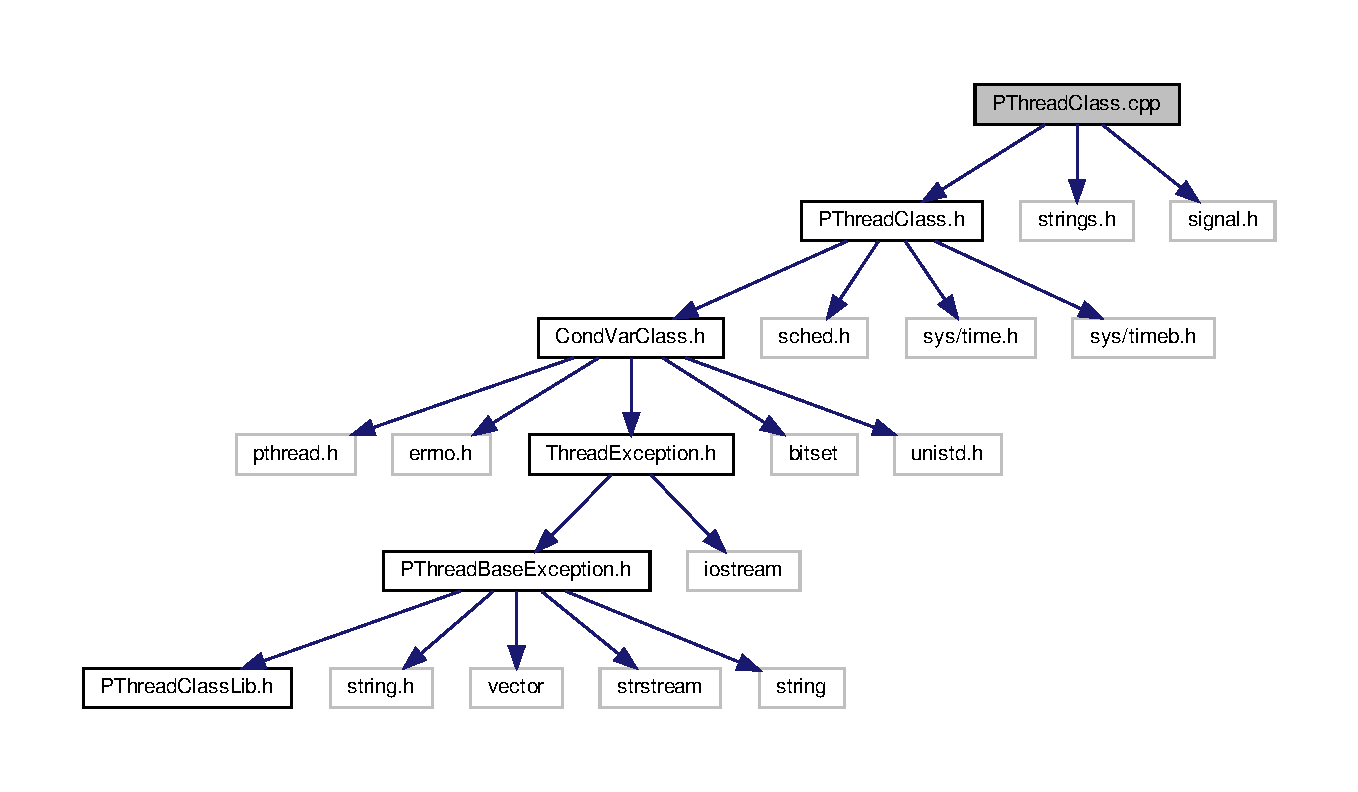
\includegraphics[width=350pt]{PThreadClass_8cpp__incl}
\end{center}
\end{figure}

\hypertarget{PThreadClass_8h}{}\section{P\+Thread\+Class.\+h File Reference}
\label{PThreadClass_8h}\index{P\+Thread\+Class.\+h@{P\+Thread\+Class.\+h}}
{\ttfamily \#include $<$Cond\+Var\+Class.\+h$>$}\newline
{\ttfamily \#include $<$sched.\+h$>$}\newline
{\ttfamily \#include $<$sys/time.\+h$>$}\newline
{\ttfamily \#include $<$sys/timeb.\+h$>$}\newline
Include dependency graph for P\+Thread\+Class.\+h\+:\nopagebreak
\begin{figure}[H]
\begin{center}
\leavevmode
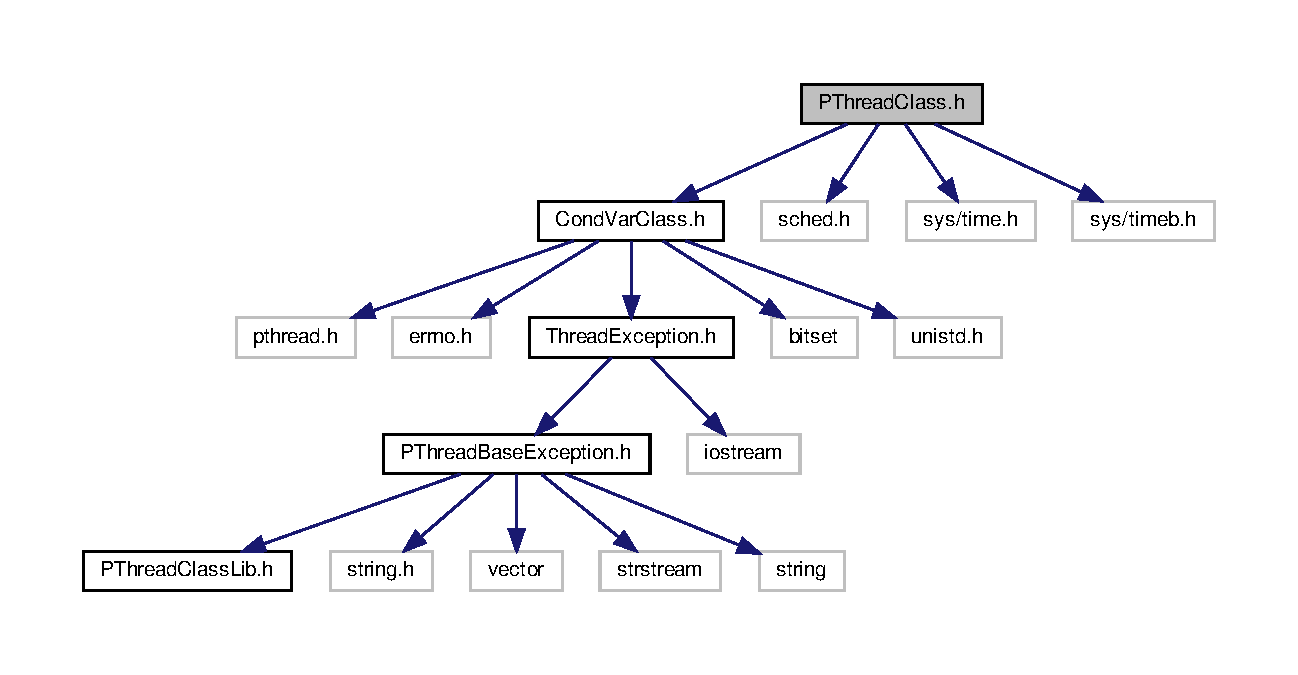
\includegraphics[width=350pt]{PThreadClass_8h__incl}
\end{center}
\end{figure}
This graph shows which files directly or indirectly include this file\+:\nopagebreak
\begin{figure}[H]
\begin{center}
\leavevmode
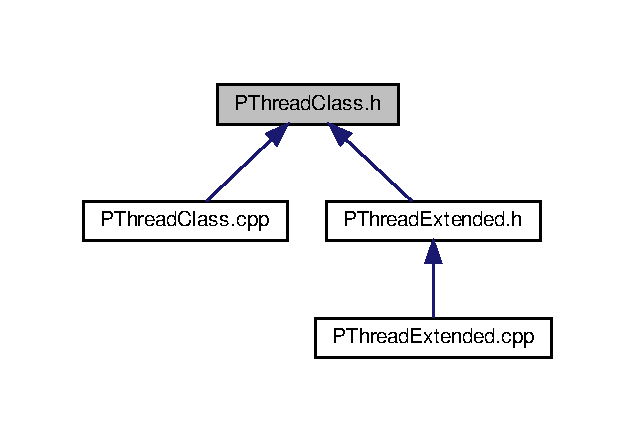
\includegraphics[width=305pt]{PThreadClass_8h__dep__incl}
\end{center}
\end{figure}
\subsection*{Classes}
\begin{DoxyCompactItemize}
\item 
struct \hyperlink{structRunnable}{Runnable}
\item 
class \hyperlink{classPThreadClass}{P\+Thread\+Class}
\end{DoxyCompactItemize}
\subsection*{Typedefs}
\begin{DoxyCompactItemize}
\item 
typedef void $\ast$($\ast$ \hyperlink{group__FUNC__DEFS_gaeef66643e734485d781ca826339879ea}{P\+Thread\+Routine\+Type}) (void $\ast$)
\item 
typedef void($\ast$ \hyperlink{group__FUNC__DEFS_ga77ca9e695666040451b77632df4847b9}{P\+Thread\+Clean\+Up\+Routine\+Type}) (void $\ast$)
\end{DoxyCompactItemize}

\hypertarget{PThreadClassLib_8cpp}{}\section{P\+Thread\+Class\+Lib.\+cpp File Reference}
\label{PThreadClassLib_8cpp}\index{P\+Thread\+Class\+Lib.\+cpp@{P\+Thread\+Class\+Lib.\+cpp}}
{\ttfamily \#include \char`\"{}P\+Thread\+Class\+Lib.\+h\char`\"{}}\newline
Include dependency graph for P\+Thread\+Class\+Lib.\+cpp\+:\nopagebreak
\begin{figure}[H]
\begin{center}
\leavevmode
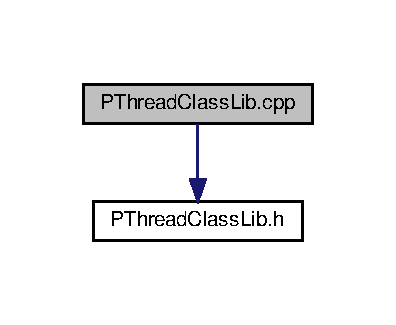
\includegraphics[width=190pt]{PThreadClassLib_8cpp__incl}
\end{center}
\end{figure}

\hypertarget{PThreadClassLib_8h}{}\section{P\+Thread\+Class\+Lib.\+h File Reference}
\label{PThreadClassLib_8h}\index{P\+Thread\+Class\+Lib.\+h@{P\+Thread\+Class\+Lib.\+h}}
This graph shows which files directly or indirectly include this file\+:\nopagebreak
\begin{figure}[H]
\begin{center}
\leavevmode
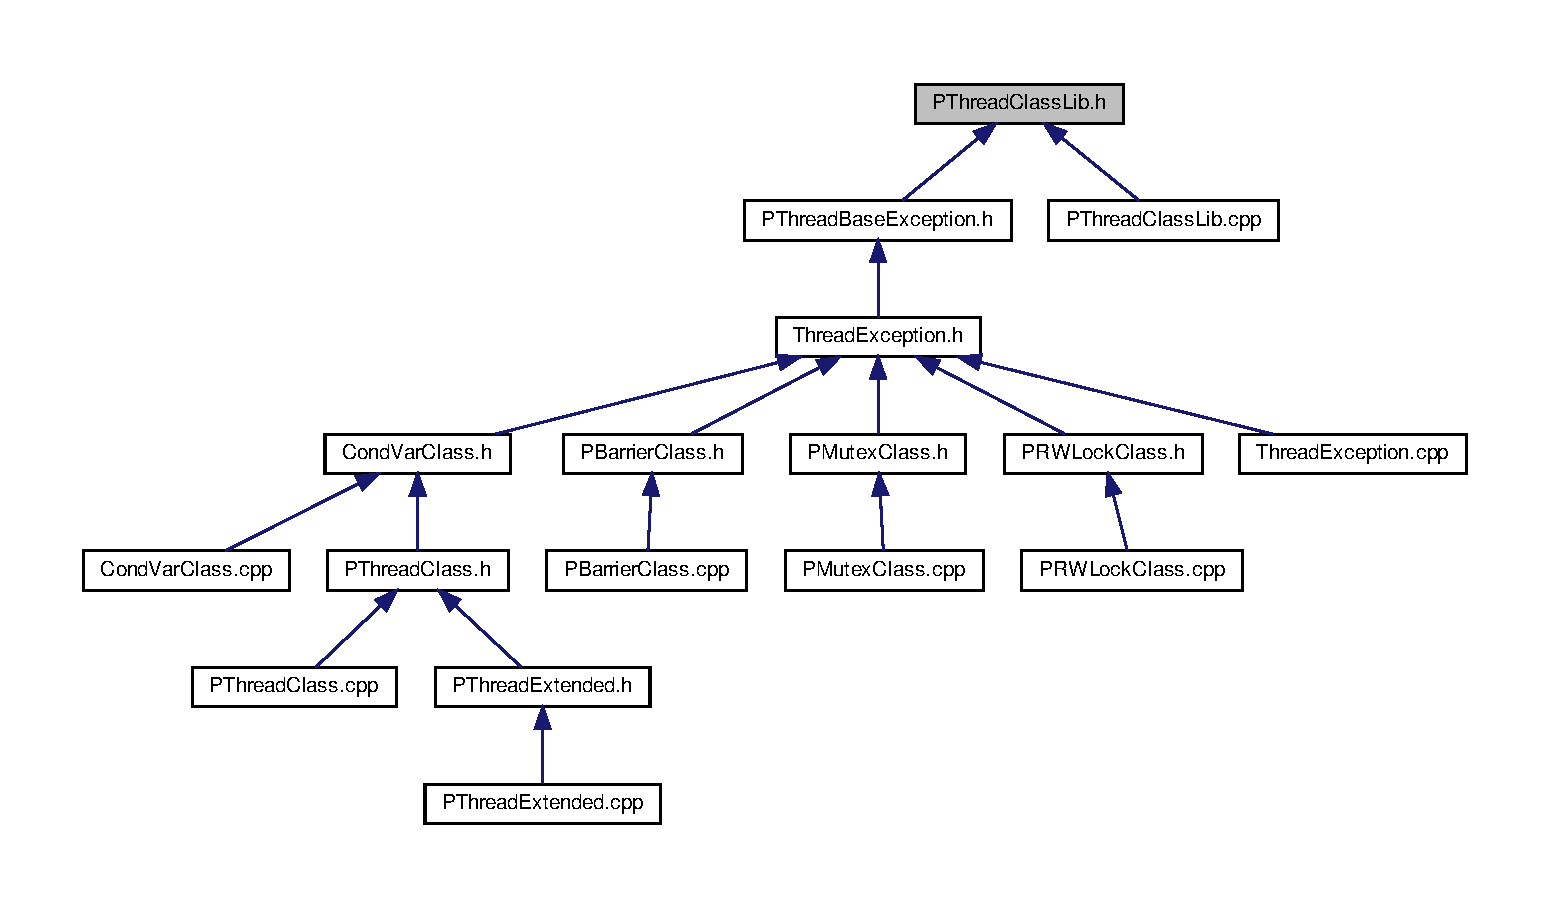
\includegraphics[width=350pt]{PThreadClassLib_8h__dep__incl}
\end{center}
\end{figure}
\subsection*{Classes}
\begin{DoxyCompactItemize}
\item 
struct \hyperlink{structPThreadClassLib_1_1VersionTriple}{P\+Thread\+Class\+Lib\+::\+Version\+Triple}
\begin{DoxyCompactList}\small\item\em Structure for library versions. \end{DoxyCompactList}\end{DoxyCompactItemize}
\subsection*{Namespaces}
\begin{DoxyCompactItemize}
\item 
 \hyperlink{namespacePThreadClassLib}{P\+Thread\+Class\+Lib}
\end{DoxyCompactItemize}
\subsection*{Macros}
\begin{DoxyCompactItemize}
\item 
\#define \hyperlink{PThreadClassLib_8h_a7a7c16bf26ea875bcbc5bd1535989b45}{P\+T\+H\+R\+E\+A\+D\+C\+L\+A\+S\+S\+L\+I\+B\+\_\+\+A\+PI}
\item 
\#define \hyperlink{PThreadClassLib_8h_a9d2d74d73cb5d069fbfcbcfebf42bd6e}{P\+T\+H\+R\+E\+A\+D\+\_\+\+I\+N\+F\+I\+N\+I\+TE}~0\+UL
\end{DoxyCompactItemize}
\subsection*{Functions}
\begin{DoxyCompactItemize}
\item 
void \hyperlink{PThreadClassLib_8h_a7a7c16bf26ea875bcbc5bd1535989b45}{P\+T\+H\+R\+E\+A\+D\+C\+L\+A\+S\+S\+L\+I\+B\+\_\+\+A\+PI} \hyperlink{group__LIB__GROUP_ga6f7b61fdb8dcf8b5602c655ac81daef8}{P\+Thread\+Class\+Lib\+::get\+Version} (Version\+Triple \&Versions)
\end{DoxyCompactItemize}


\subsection{Macro Definition Documentation}
\mbox{\Hypertarget{PThreadClassLib_8h_a9d2d74d73cb5d069fbfcbcfebf42bd6e}\label{PThreadClassLib_8h_a9d2d74d73cb5d069fbfcbcfebf42bd6e}} 
\index{P\+Thread\+Class\+Lib.\+h@{P\+Thread\+Class\+Lib.\+h}!P\+T\+H\+R\+E\+A\+D\+\_\+\+I\+N\+F\+I\+N\+I\+TE@{P\+T\+H\+R\+E\+A\+D\+\_\+\+I\+N\+F\+I\+N\+I\+TE}}
\index{P\+T\+H\+R\+E\+A\+D\+\_\+\+I\+N\+F\+I\+N\+I\+TE@{P\+T\+H\+R\+E\+A\+D\+\_\+\+I\+N\+F\+I\+N\+I\+TE}!P\+Thread\+Class\+Lib.\+h@{P\+Thread\+Class\+Lib.\+h}}
\subsubsection{\texorpdfstring{P\+T\+H\+R\+E\+A\+D\+\_\+\+I\+N\+F\+I\+N\+I\+TE}{PTHREAD\_INFINITE}}
{\footnotesize\ttfamily \#define P\+T\+H\+R\+E\+A\+D\+\_\+\+I\+N\+F\+I\+N\+I\+TE~0\+UL}

\mbox{\Hypertarget{PThreadClassLib_8h_a7a7c16bf26ea875bcbc5bd1535989b45}\label{PThreadClassLib_8h_a7a7c16bf26ea875bcbc5bd1535989b45}} 
\index{P\+Thread\+Class\+Lib.\+h@{P\+Thread\+Class\+Lib.\+h}!P\+T\+H\+R\+E\+A\+D\+C\+L\+A\+S\+S\+L\+I\+B\+\_\+\+A\+PI@{P\+T\+H\+R\+E\+A\+D\+C\+L\+A\+S\+S\+L\+I\+B\+\_\+\+A\+PI}}
\index{P\+T\+H\+R\+E\+A\+D\+C\+L\+A\+S\+S\+L\+I\+B\+\_\+\+A\+PI@{P\+T\+H\+R\+E\+A\+D\+C\+L\+A\+S\+S\+L\+I\+B\+\_\+\+A\+PI}!P\+Thread\+Class\+Lib.\+h@{P\+Thread\+Class\+Lib.\+h}}
\subsubsection{\texorpdfstring{P\+T\+H\+R\+E\+A\+D\+C\+L\+A\+S\+S\+L\+I\+B\+\_\+\+A\+PI}{PTHREADCLASSLIB\_API}}
{\footnotesize\ttfamily \#define P\+T\+H\+R\+E\+A\+D\+C\+L\+A\+S\+S\+L\+I\+B\+\_\+\+A\+PI}


\hypertarget{pthreadclasslib__global_8h}{}\section{pthreadclasslib\+\_\+global.\+h File Reference}
\label{pthreadclasslib__global_8h}\index{pthreadclasslib\+\_\+global.\+h@{pthreadclasslib\+\_\+global.\+h}}
{\ttfamily \#include $<$Qt\+Core/qglobal.\+h$>$}\newline
Include dependency graph for pthreadclasslib\+\_\+global.\+h\+:\nopagebreak
\begin{figure}[H]
\begin{center}
\leavevmode
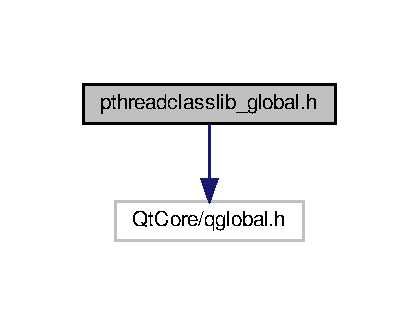
\includegraphics[width=201pt]{pthreadclasslib__global_8h__incl}
\end{center}
\end{figure}
\subsection*{Macros}
\begin{DoxyCompactItemize}
\item 
\#define \hyperlink{pthreadclasslib__global_8h_a544bda5912312d610aee7188039073ba}{P\+T\+H\+R\+E\+A\+D\+C\+L\+A\+S\+S\+L\+I\+B\+S\+H\+A\+R\+E\+D\+\_\+\+E\+X\+P\+O\+RT}~Q\+\_\+\+D\+E\+C\+L\+\_\+\+I\+M\+P\+O\+RT
\end{DoxyCompactItemize}


\subsection{Macro Definition Documentation}
\mbox{\Hypertarget{pthreadclasslib__global_8h_a544bda5912312d610aee7188039073ba}\label{pthreadclasslib__global_8h_a544bda5912312d610aee7188039073ba}} 
\index{pthreadclasslib\+\_\+global.\+h@{pthreadclasslib\+\_\+global.\+h}!P\+T\+H\+R\+E\+A\+D\+C\+L\+A\+S\+S\+L\+I\+B\+S\+H\+A\+R\+E\+D\+\_\+\+E\+X\+P\+O\+RT@{P\+T\+H\+R\+E\+A\+D\+C\+L\+A\+S\+S\+L\+I\+B\+S\+H\+A\+R\+E\+D\+\_\+\+E\+X\+P\+O\+RT}}
\index{P\+T\+H\+R\+E\+A\+D\+C\+L\+A\+S\+S\+L\+I\+B\+S\+H\+A\+R\+E\+D\+\_\+\+E\+X\+P\+O\+RT@{P\+T\+H\+R\+E\+A\+D\+C\+L\+A\+S\+S\+L\+I\+B\+S\+H\+A\+R\+E\+D\+\_\+\+E\+X\+P\+O\+RT}!pthreadclasslib\+\_\+global.\+h@{pthreadclasslib\+\_\+global.\+h}}
\subsubsection{\texorpdfstring{P\+T\+H\+R\+E\+A\+D\+C\+L\+A\+S\+S\+L\+I\+B\+S\+H\+A\+R\+E\+D\+\_\+\+E\+X\+P\+O\+RT}{PTHREADCLASSLIBSHARED\_EXPORT}}
{\footnotesize\ttfamily \#define P\+T\+H\+R\+E\+A\+D\+C\+L\+A\+S\+S\+L\+I\+B\+S\+H\+A\+R\+E\+D\+\_\+\+E\+X\+P\+O\+RT~Q\+\_\+\+D\+E\+C\+L\+\_\+\+I\+M\+P\+O\+RT}


\hypertarget{PThreadExtended_8cpp}{}\section{P\+Thread\+Extended.\+cpp File Reference}
\label{PThreadExtended_8cpp}\index{P\+Thread\+Extended.\+cpp@{P\+Thread\+Extended.\+cpp}}
{\ttfamily \#include $<$P\+Thread\+Extended.\+h$>$}\newline
Include dependency graph for P\+Thread\+Extended.\+cpp\+:\nopagebreak
\begin{figure}[H]
\begin{center}
\leavevmode
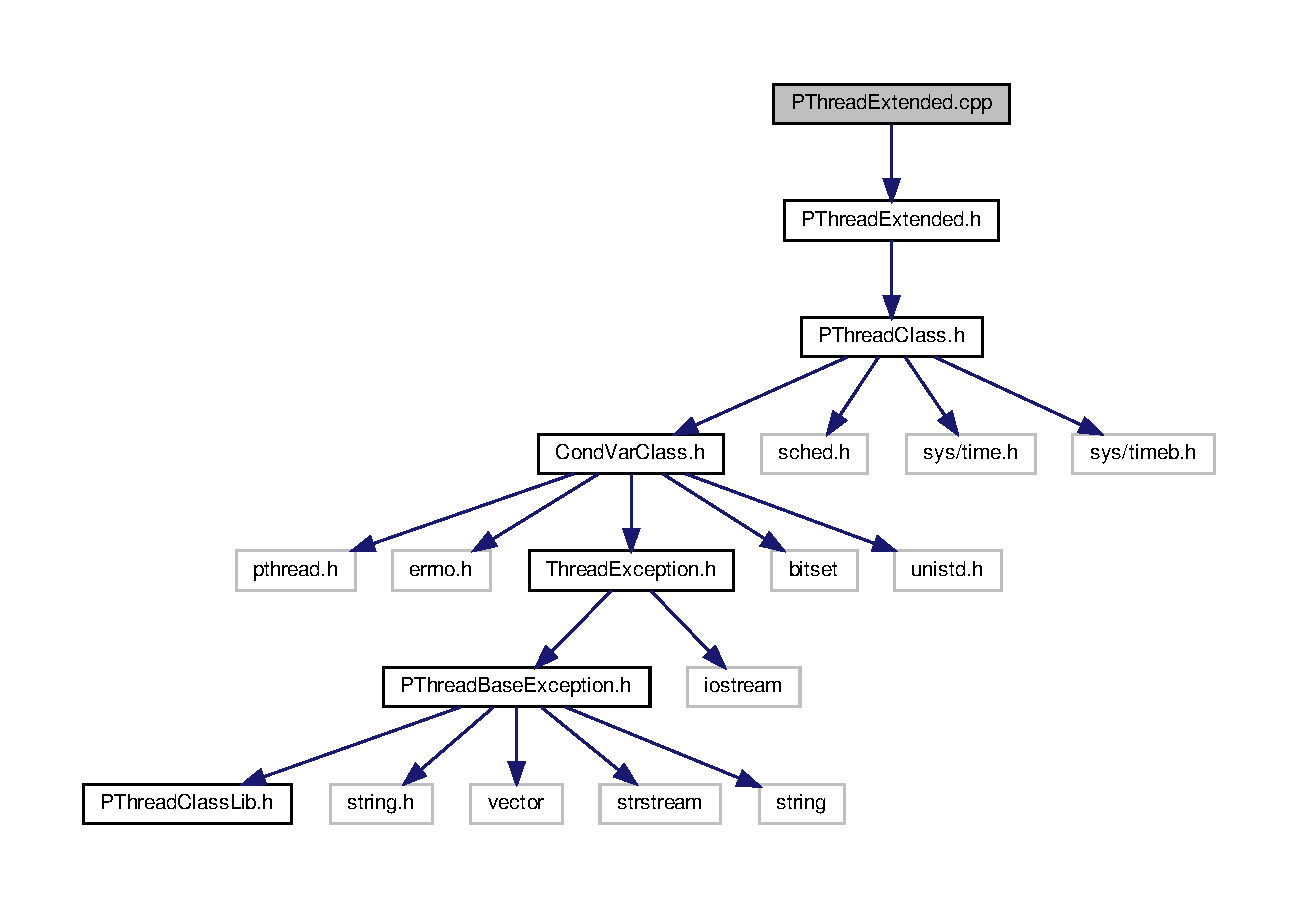
\includegraphics[width=350pt]{PThreadExtended_8cpp__incl}
\end{center}
\end{figure}

\hypertarget{PThreadExtended_8h}{}\section{P\+Thread\+Extended.\+h File Reference}
\label{PThreadExtended_8h}\index{P\+Thread\+Extended.\+h@{P\+Thread\+Extended.\+h}}
{\ttfamily \#include $<$P\+Thread\+Class.\+h$>$}\newline
Include dependency graph for P\+Thread\+Extended.\+h\+:\nopagebreak
\begin{figure}[H]
\begin{center}
\leavevmode
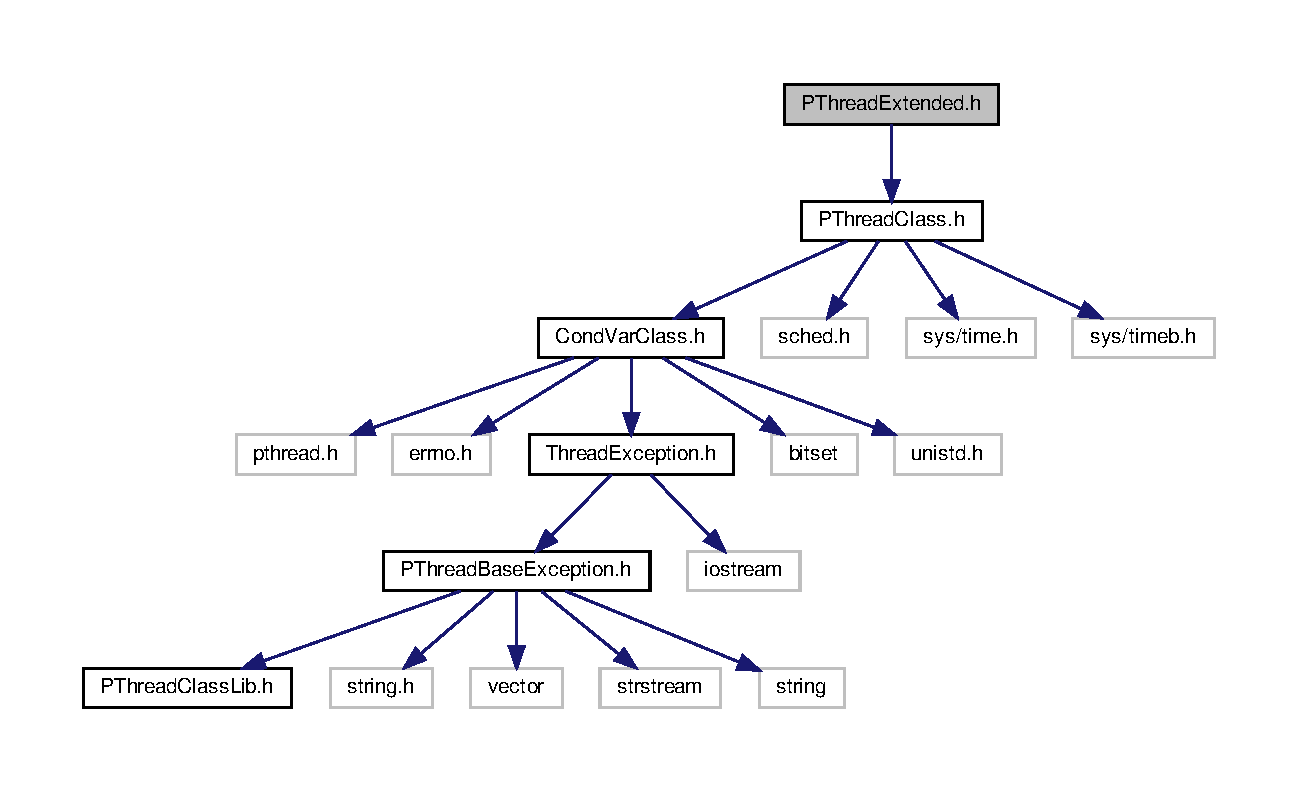
\includegraphics[width=350pt]{PThreadExtended_8h__incl}
\end{center}
\end{figure}
This graph shows which files directly or indirectly include this file\+:\nopagebreak
\begin{figure}[H]
\begin{center}
\leavevmode
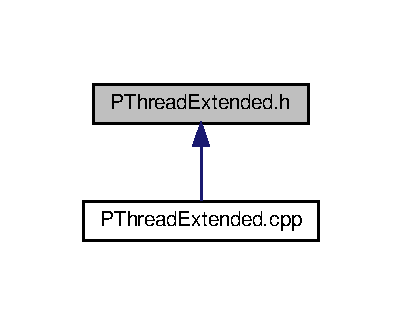
\includegraphics[width=193pt]{PThreadExtended_8h__dep__incl}
\end{center}
\end{figure}
\subsection*{Classes}
\begin{DoxyCompactItemize}
\item 
class \hyperlink{classPThreadExtended}{P\+Thread\+Extended}
\end{DoxyCompactItemize}
\subsection*{Typedefs}
\begin{DoxyCompactItemize}
\item 
typedef void($\ast$ \hyperlink{group__FUNC__DEFS_ga164076b53d35e4dba4c51bb336c15dab}{P\+Thread\+Notification\+Func\+Type}) (void $\ast$)
\end{DoxyCompactItemize}

\hypertarget{ThreadException_8cpp}{}\section{Thread\+Exception.\+cpp File Reference}
\label{ThreadException_8cpp}\index{Thread\+Exception.\+cpp@{Thread\+Exception.\+cpp}}
{\ttfamily \#include $<$Thread\+Exception.\+h$>$}\newline
Include dependency graph for Thread\+Exception.\+cpp\+:\nopagebreak
\begin{figure}[H]
\begin{center}
\leavevmode
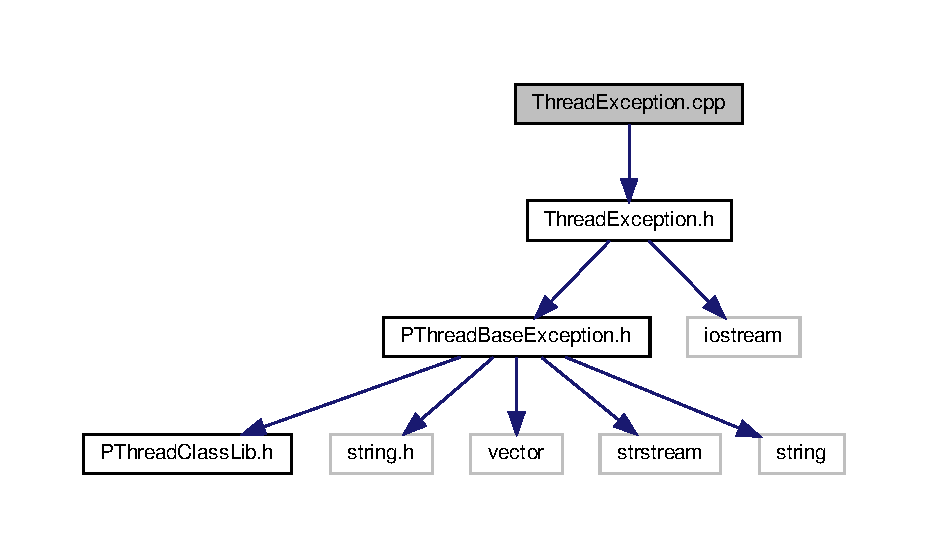
\includegraphics[width=350pt]{ThreadException_8cpp__incl}
\end{center}
\end{figure}

\hypertarget{ThreadException_8h}{}\section{Thread\+Exception.\+h File Reference}
\label{ThreadException_8h}\index{Thread\+Exception.\+h@{Thread\+Exception.\+h}}
{\ttfamily \#include $<$P\+Thread\+Base\+Exception.\+h$>$}\newline
{\ttfamily \#include $<$iostream$>$}\newline
Include dependency graph for Thread\+Exception.\+h\+:\nopagebreak
\begin{figure}[H]
\begin{center}
\leavevmode
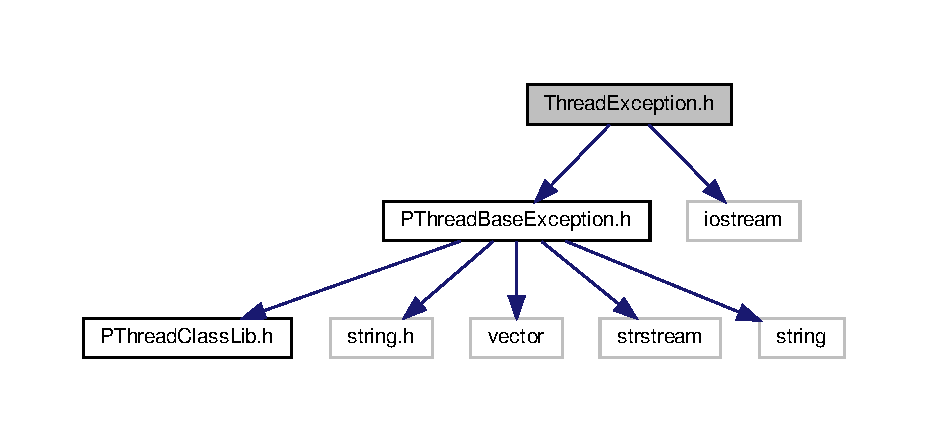
\includegraphics[width=350pt]{ThreadException_8h__incl}
\end{center}
\end{figure}
This graph shows which files directly or indirectly include this file\+:\nopagebreak
\begin{figure}[H]
\begin{center}
\leavevmode
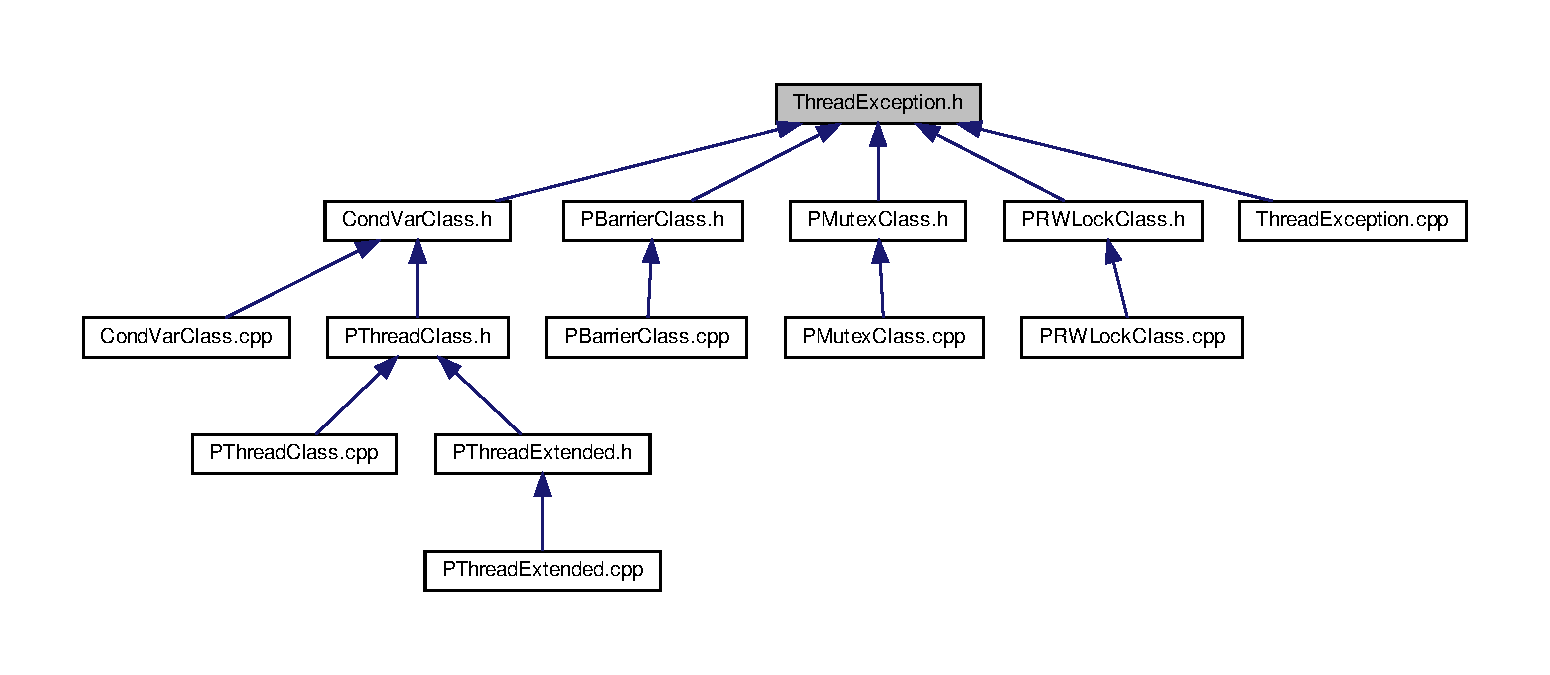
\includegraphics[width=350pt]{ThreadException_8h__dep__incl}
\end{center}
\end{figure}
\subsection*{Classes}
\begin{DoxyCompactItemize}
\item 
class \hyperlink{classThreadException}{Thread\+Exception}
\end{DoxyCompactItemize}
\subsection*{Macros}
\begin{DoxyCompactItemize}
\item 
\#define \hyperlink{group__EXCEPT__GROUP_ga5db5dc006d9e017998d2def9ce105503}{T\+H\+R\+E\+A\+D\+\_\+\+E\+X\+C\+E\+P\+T\+\_\+\+T\+H\+R\+OW}(x)
\begin{DoxyCompactList}\small\item\em Throw exception based on filename and line number. \end{DoxyCompactList}\item 
\#define \hyperlink{group__EXCEPT__GROUP_ga30ed89be31363fd6edbdf69c667f6a6e}{T\+H\+R\+E\+A\+D\+\_\+\+E\+X\+C\+E\+P\+T\+\_\+\+C\+A\+T\+C\+H\+\_\+\+A\+N\+D\+\_\+\+R\+A\+I\+SE}(x)
\begin{DoxyCompactList}\small\item\em Catch and re-\/throw an exception. \end{DoxyCompactList}\item 
\#define \hyperlink{group__EXCEPT__GROUP_ga0c52d227f70b6081ba66c3139a4e93f4}{T\+H\+R\+E\+A\+D\+\_\+\+E\+X\+C\+E\+P\+T\+\_\+\+C\+A\+T\+C\+H\+\_\+\+B\+E\+G\+I\+N\+\_\+\+N\+O\+R\+EP}
\begin{DoxyCompactList}\small\item\em Begin catch block with no reporter. \end{DoxyCompactList}\item 
\#define \hyperlink{group__EXCEPT__GROUP_gaf7630fb76915f40ee3d6f7499a20671d}{T\+H\+R\+E\+A\+D\+\_\+\+E\+X\+C\+E\+P\+T\+\_\+\+C\+A\+T\+C\+H\+\_\+\+B\+E\+G\+IN}(x)
\begin{DoxyCompactList}\small\item\em Begin catch block. \end{DoxyCompactList}\item 
\#define \hyperlink{group__EXCEPT__GROUP_gac9a9fa6b62369772230ad12ff2b51e89}{T\+H\+R\+E\+A\+D\+\_\+\+E\+X\+C\+E\+P\+T\+\_\+\+C\+A\+T\+C\+H\+\_\+\+A\+LL}(x)
\begin{DoxyCompactList}\small\item\em Catch all -\/ aka catch(...). \end{DoxyCompactList}\item 
\#define \hyperlink{group__EXCEPT__GROUP_gab885e9554b19d207b874259b5c5fd9be}{T\+H\+R\+E\+A\+D\+\_\+\+E\+X\+C\+E\+P\+T\+\_\+\+C\+A\+T\+C\+H\+\_\+\+E\+ND}~\}
\begin{DoxyCompactList}\small\item\em End catch block. \end{DoxyCompactList}\item 
\#define \hyperlink{group__EXCEPT__GROUP_ga517202bf1ba7e87014662a560bbcb43c}{T\+H\+R\+E\+A\+D\+\_\+\+T\+RY}~try
\begin{DoxyCompactList}\small\item\em Begin try block. \end{DoxyCompactList}\end{DoxyCompactItemize}

%--- End generated contents ---

% Index
\backmatter
\newpage
\phantomsection
\clearemptydoublepage
\addcontentsline{toc}{chapter}{Index}
\printindex

\end{document}
